\documentclass[fleqn,12pt]{supp}
%%\usepackage{setspace}
%%\doublespacing
\usepackage{soul, float, hyperref}
\hypersetup{hidelinks}
\usepackage[utf8]{inputenc}

\newcommand{\beginsupplement}{%
        \setcounter{table}{0}
        \renewcommand{\thetable}{S\arabic{table}}%
        \setcounter{figure}{0}
        \renewcommand{\thefigure}{S\arabic{figure}}%
     }

\title{Supplementary Information}
\author{}

\begin{document}

\flushbottom
\maketitle

\vspace{-35pt}
\section*{A Structural and Functional Bioinformatics Study of QTY-designed Retinylidene Proteins}

\subsection*{Siqi Pan and Shuguang Zhang}

\begin{figure}[H]
    \caption{\textbf{The enlarge protein sequence alignments of 12 retinylidene proteins with their water-soluble QTY analogs from Figure 1.} The symbols $|$ and $*$ indicate that amino acids are identical and different respectively. Amino acids L, V, I and F in TM (transmembrane) alpha helices are replaced with Q, T, Y and Y respectively. The alpha helices (blue) are shown above the protein sequences. \\
    The alignments are: 
    \textbf{a)} OPN1MW \textit{vs} OPN1MW$^{\textrm{QTY}}$, 
    \textbf{b)} OPN1LW \textit{vs} OPN1LW$^{\textrm{QTY}}$, 
    \textbf{c)} OPN1SW \textit{vs} OPN1SW$^{\textrm{QTY}}$, 
    \textbf{d)} OPN2 \textit{vs} OPN2$^{\textrm{QTY}}$, 
    \textbf{e)} OPN3 \textit{vs} OPN3$^{\textrm{QTY}}$, 
    \textbf{f)} OPN4 \textit{vs} OPN4$^{\textrm{QTY}}$, 
    \textbf{g)} OPN5 \textit{vs} OPN5$^{\textrm{QTY}}$, 
    \textbf{h)} RGR \textit{vs} RGR$^{\textrm{QTY}}$, 
    \textbf{i)} RRH \textit{vs} RRH$^{\textrm{QTY}}$, 
    \textbf{j)} BACR \textit{vs} BACR$^{\textrm{QTY}}$, 
    \textbf{k)} BACH \textit{vs} BACH$^{\textrm{QTY}}$, 
    \textbf{l)} ChR2 \textit{vs} ChR2$^{\textrm{QTY}}$. }
    \textbf{a)} OPN1MW \textit{vs} OPN1MW$^{\textrm{QTY}}$ \\
    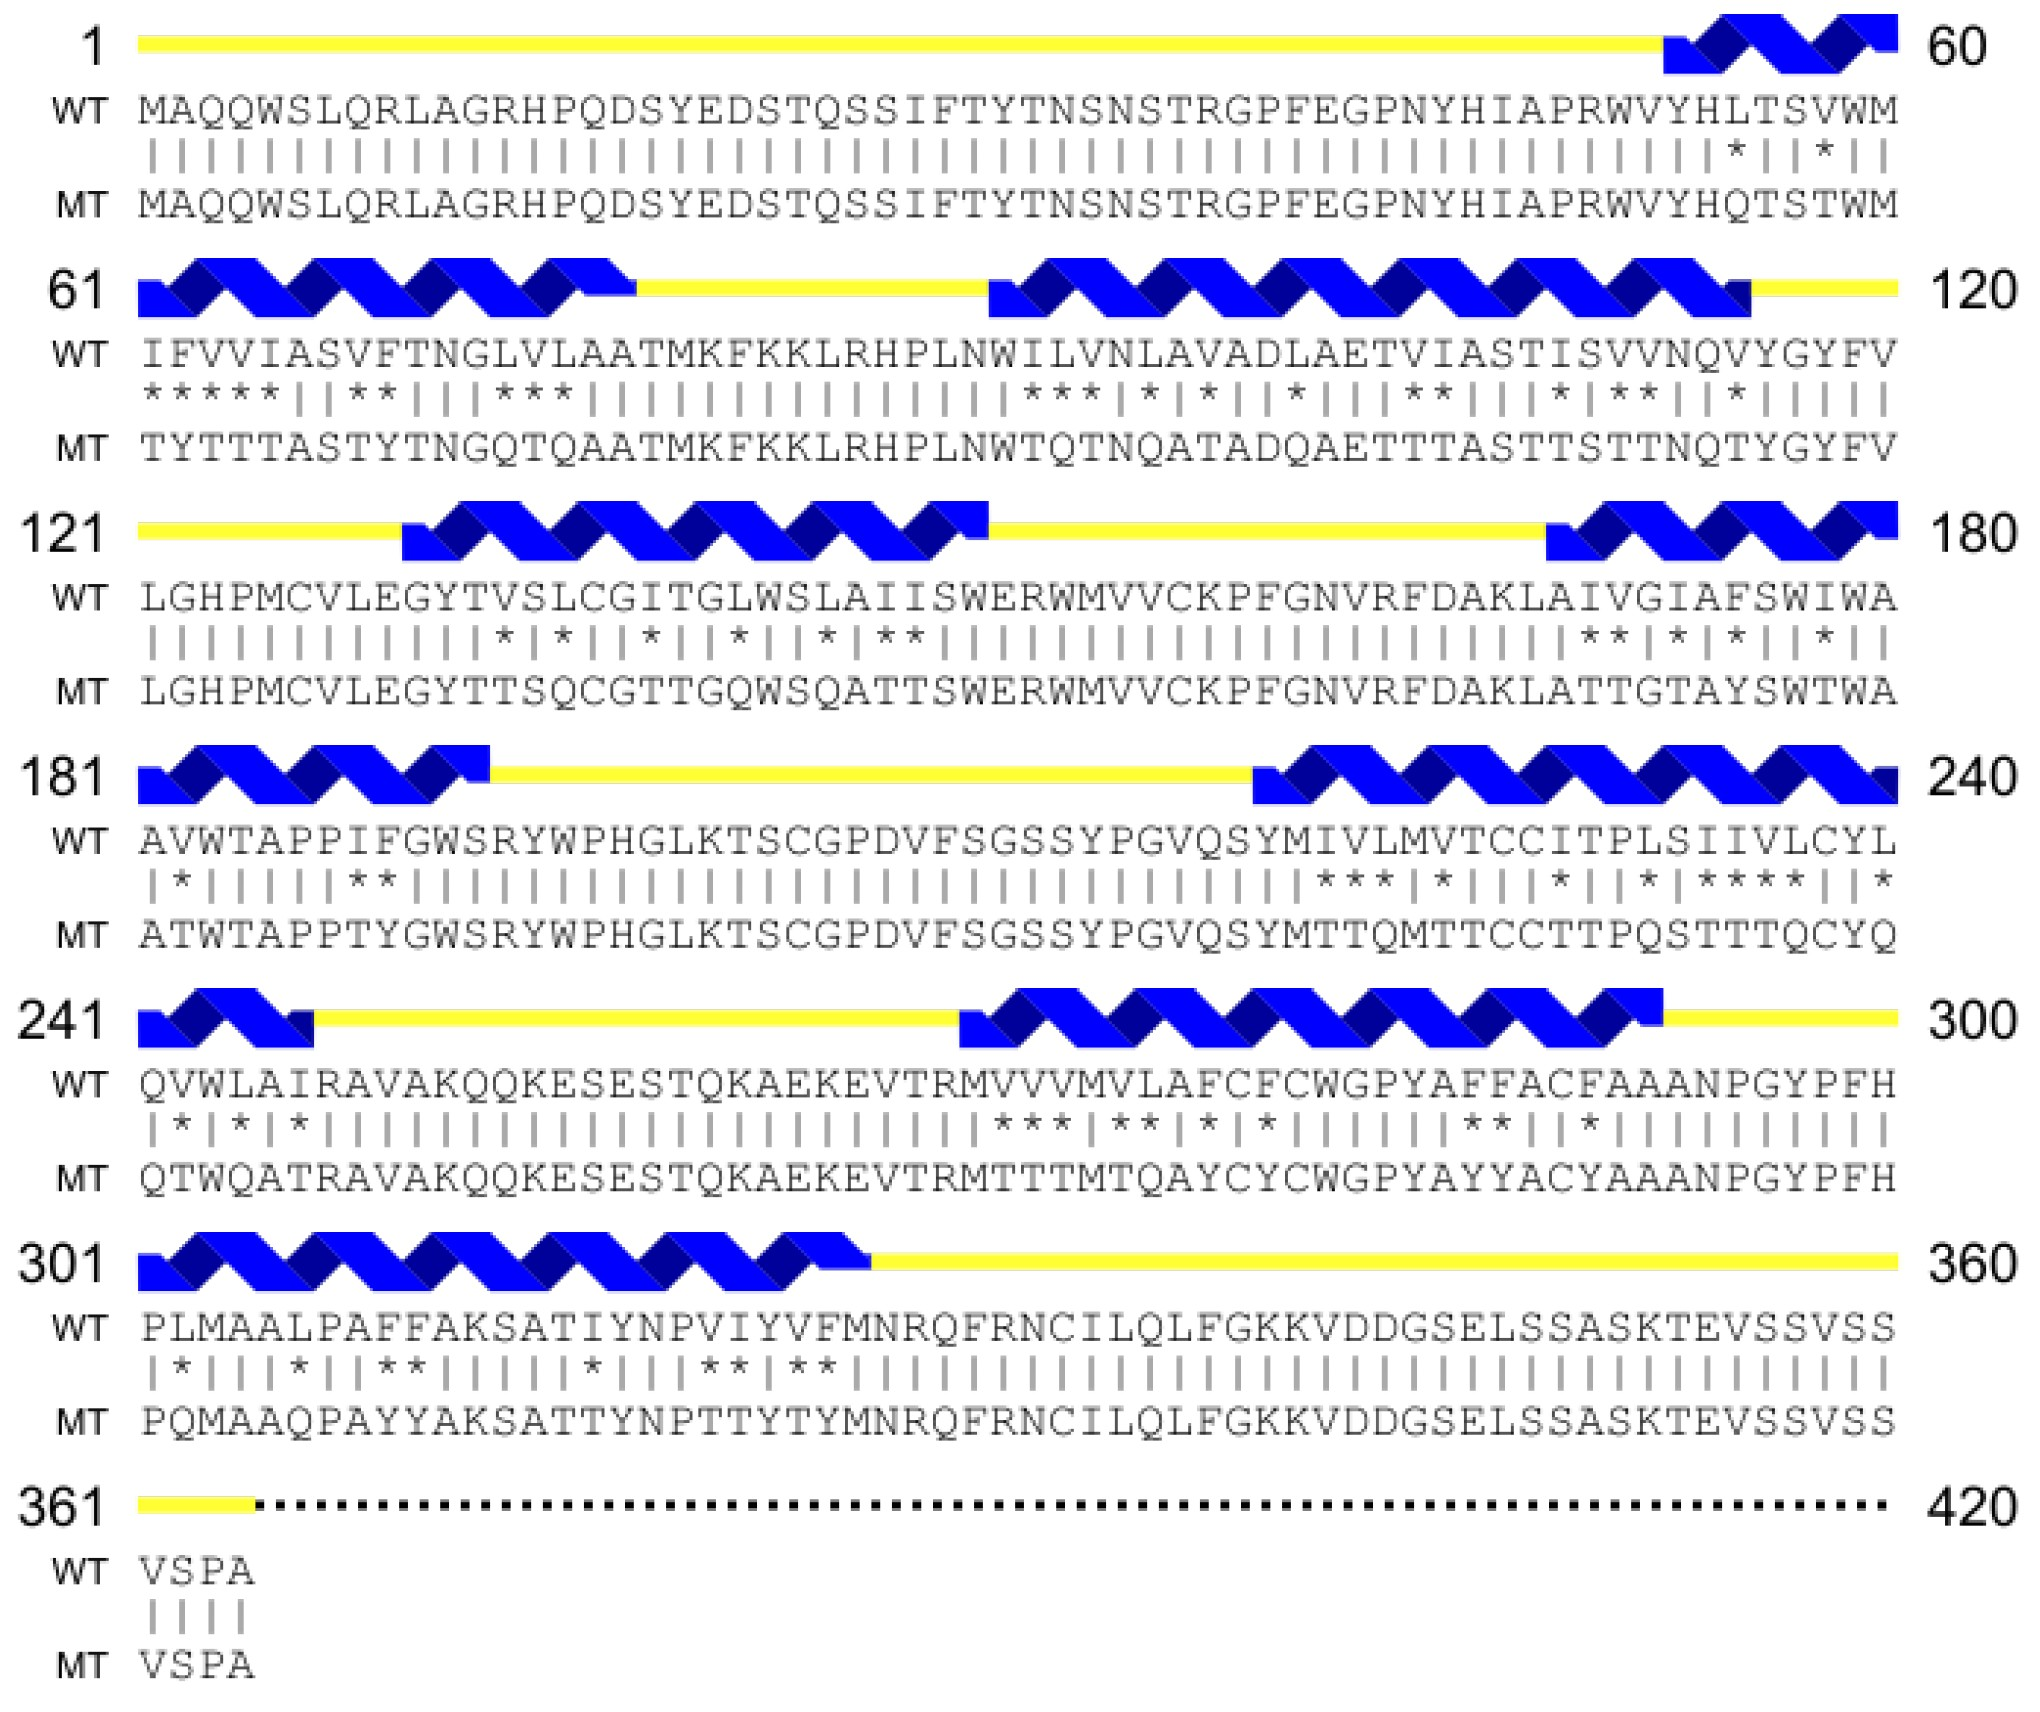
\includegraphics[width=\linewidth]{SuppFigures/opn1mw.jpg}
\end{figure}

\newpage
\begin{figure}[H]
    \textbf{b)} OPN1LW \textit{vs} OPN1LW$^{\textrm{QTY}}$ \\
    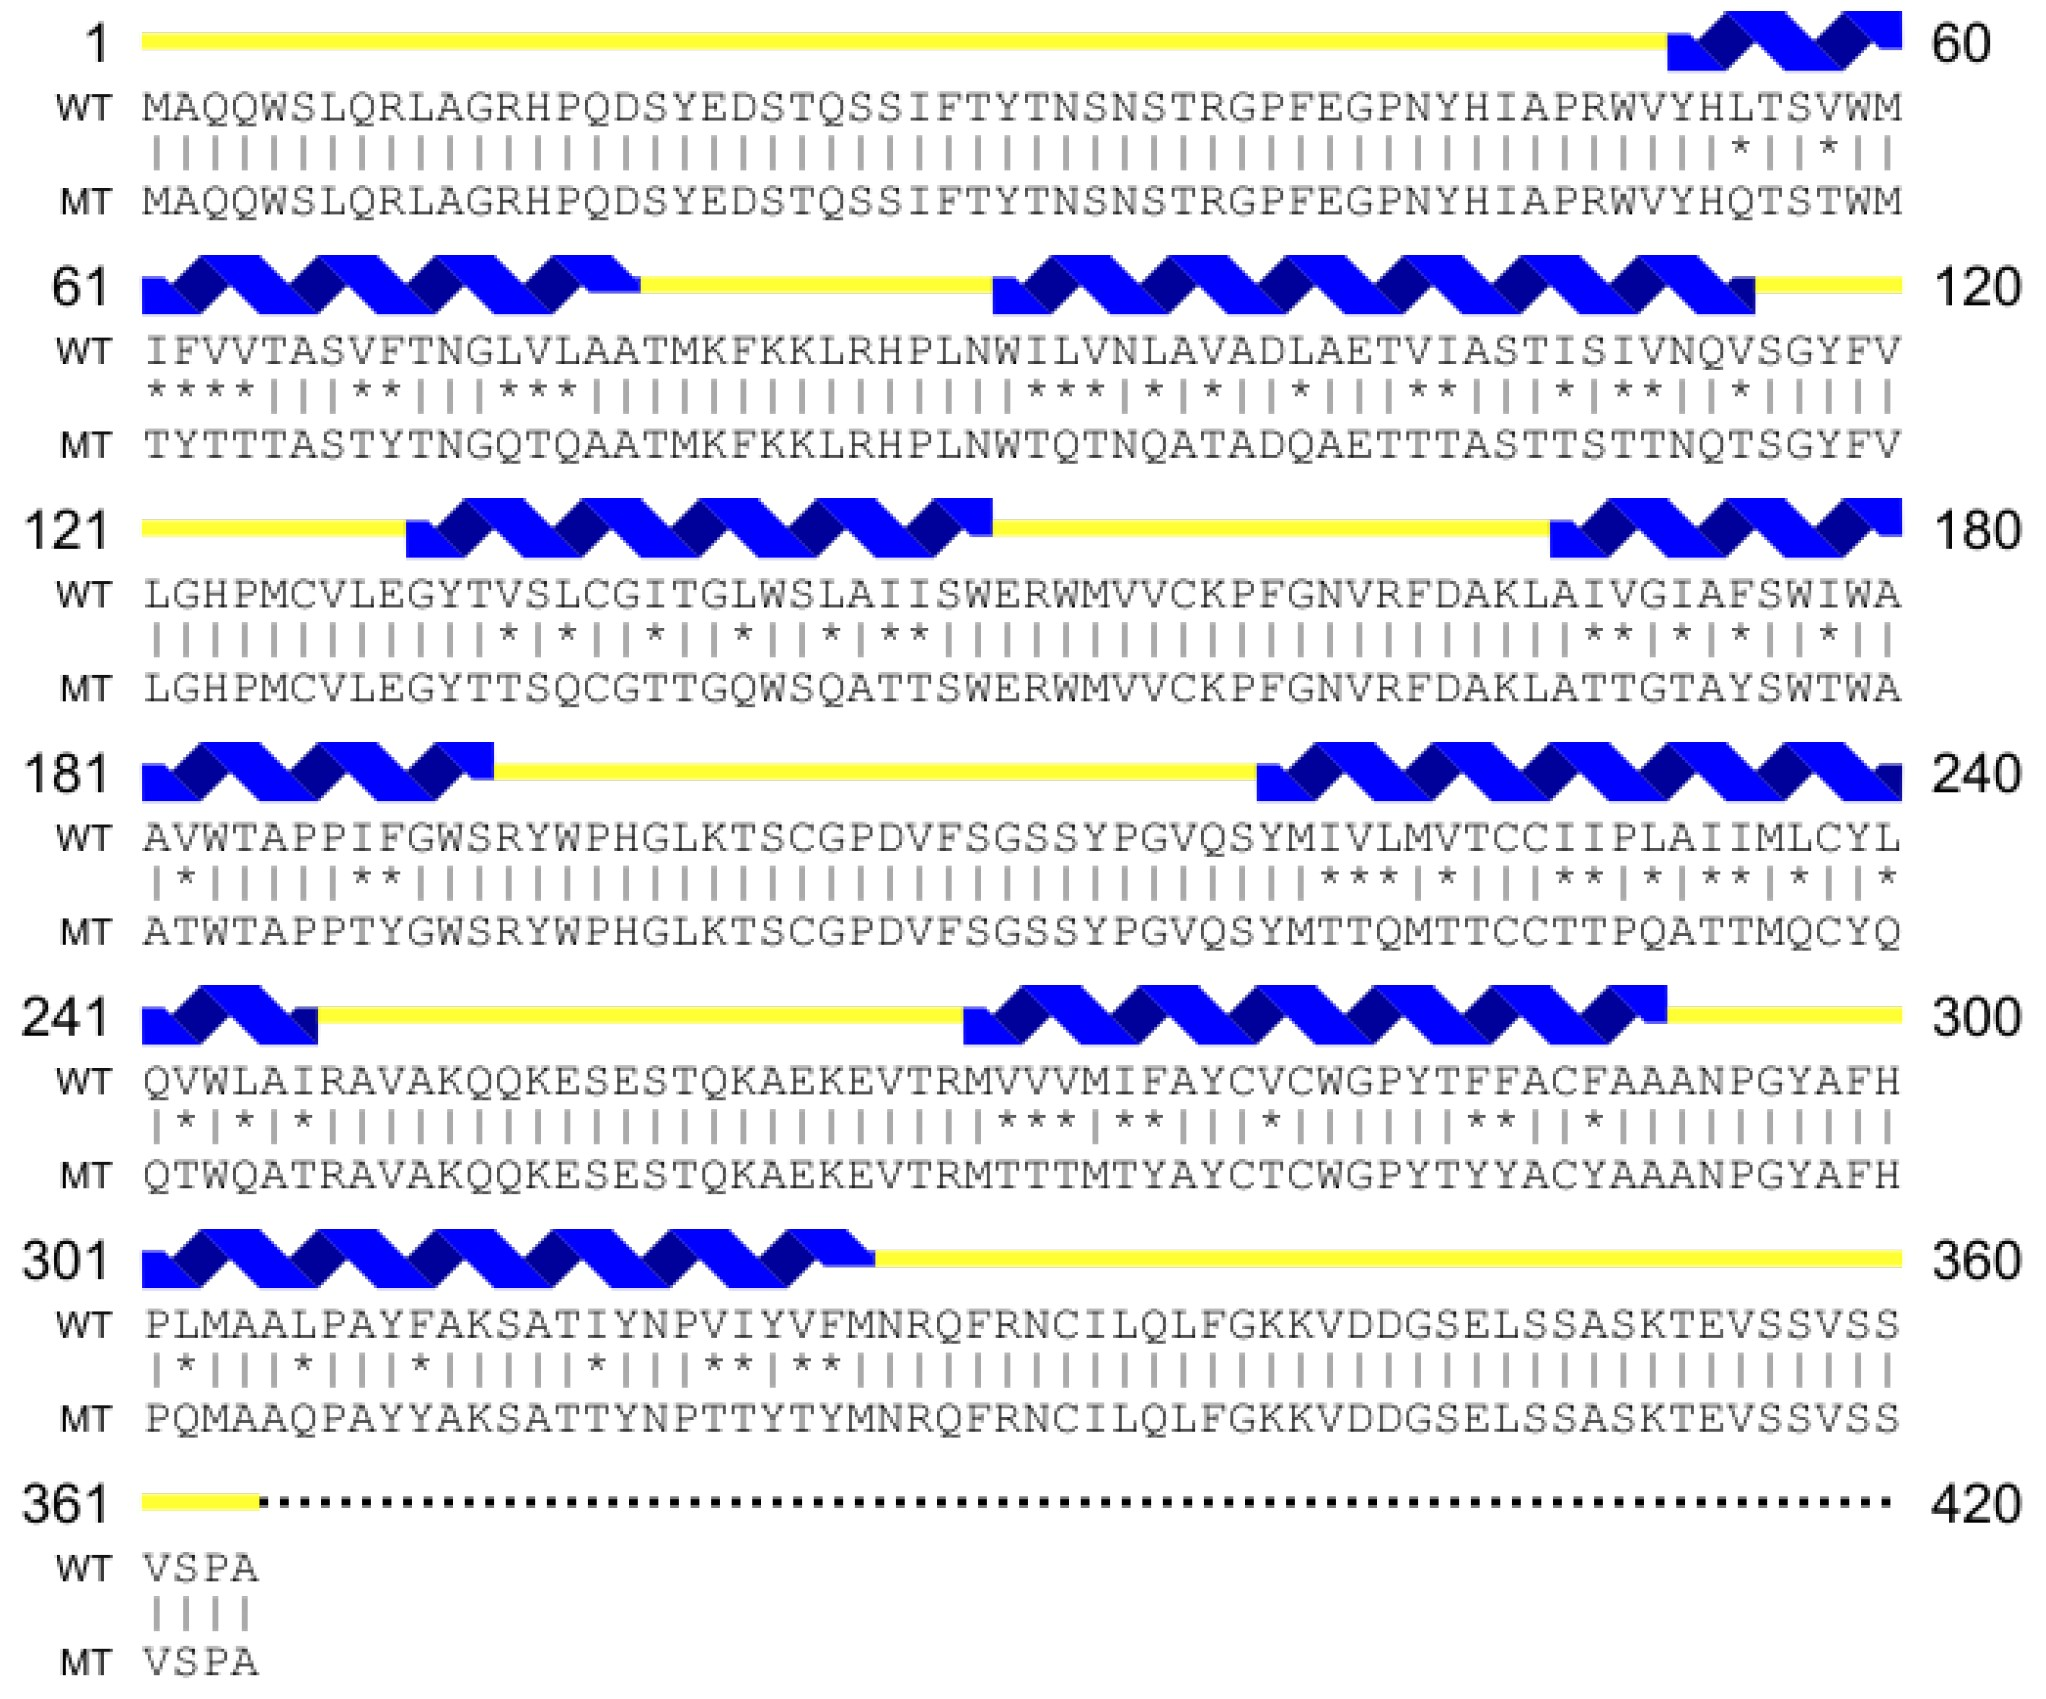
\includegraphics[width=\linewidth]{SuppFigures/opn1lw.jpg}
\end{figure}

\newpage
\begin{figure}[H]
    \textbf{c)} OPN1SW \textit{vs} OPN1SW$^{\textrm{QTY}}$ \\
    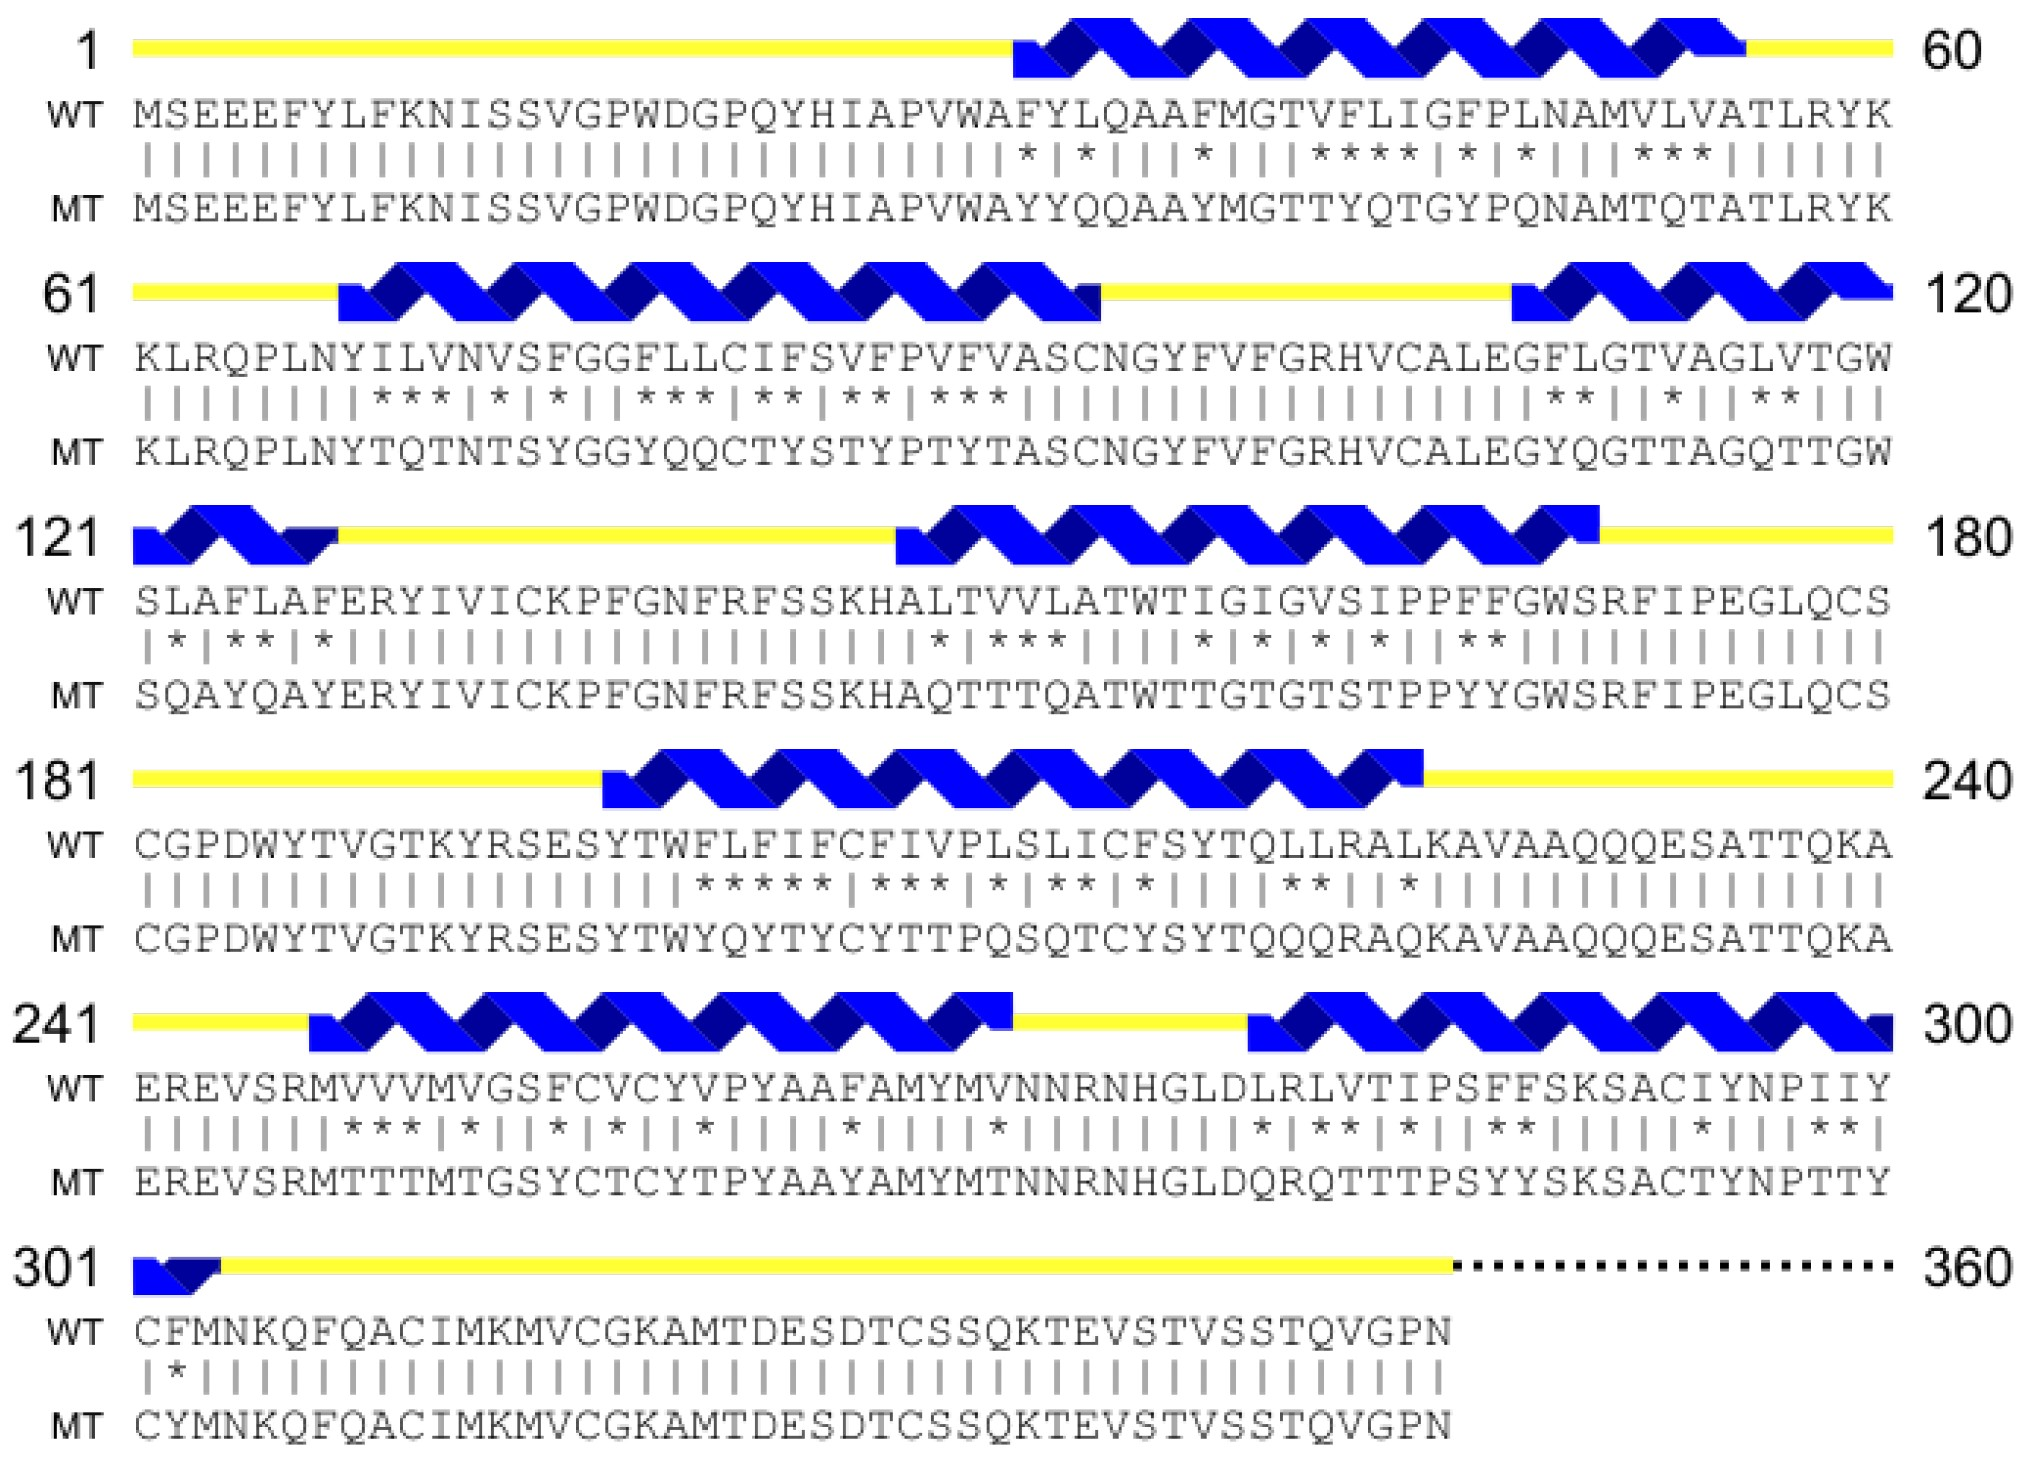
\includegraphics[width=\linewidth]{SuppFigures/opn1sw.jpg}
\end{figure}

\newpage
\begin{figure}[H]
    \textbf{d)} OPN2 \textit{vs} OPN2$^{\textrm{QTY}}$ \\
    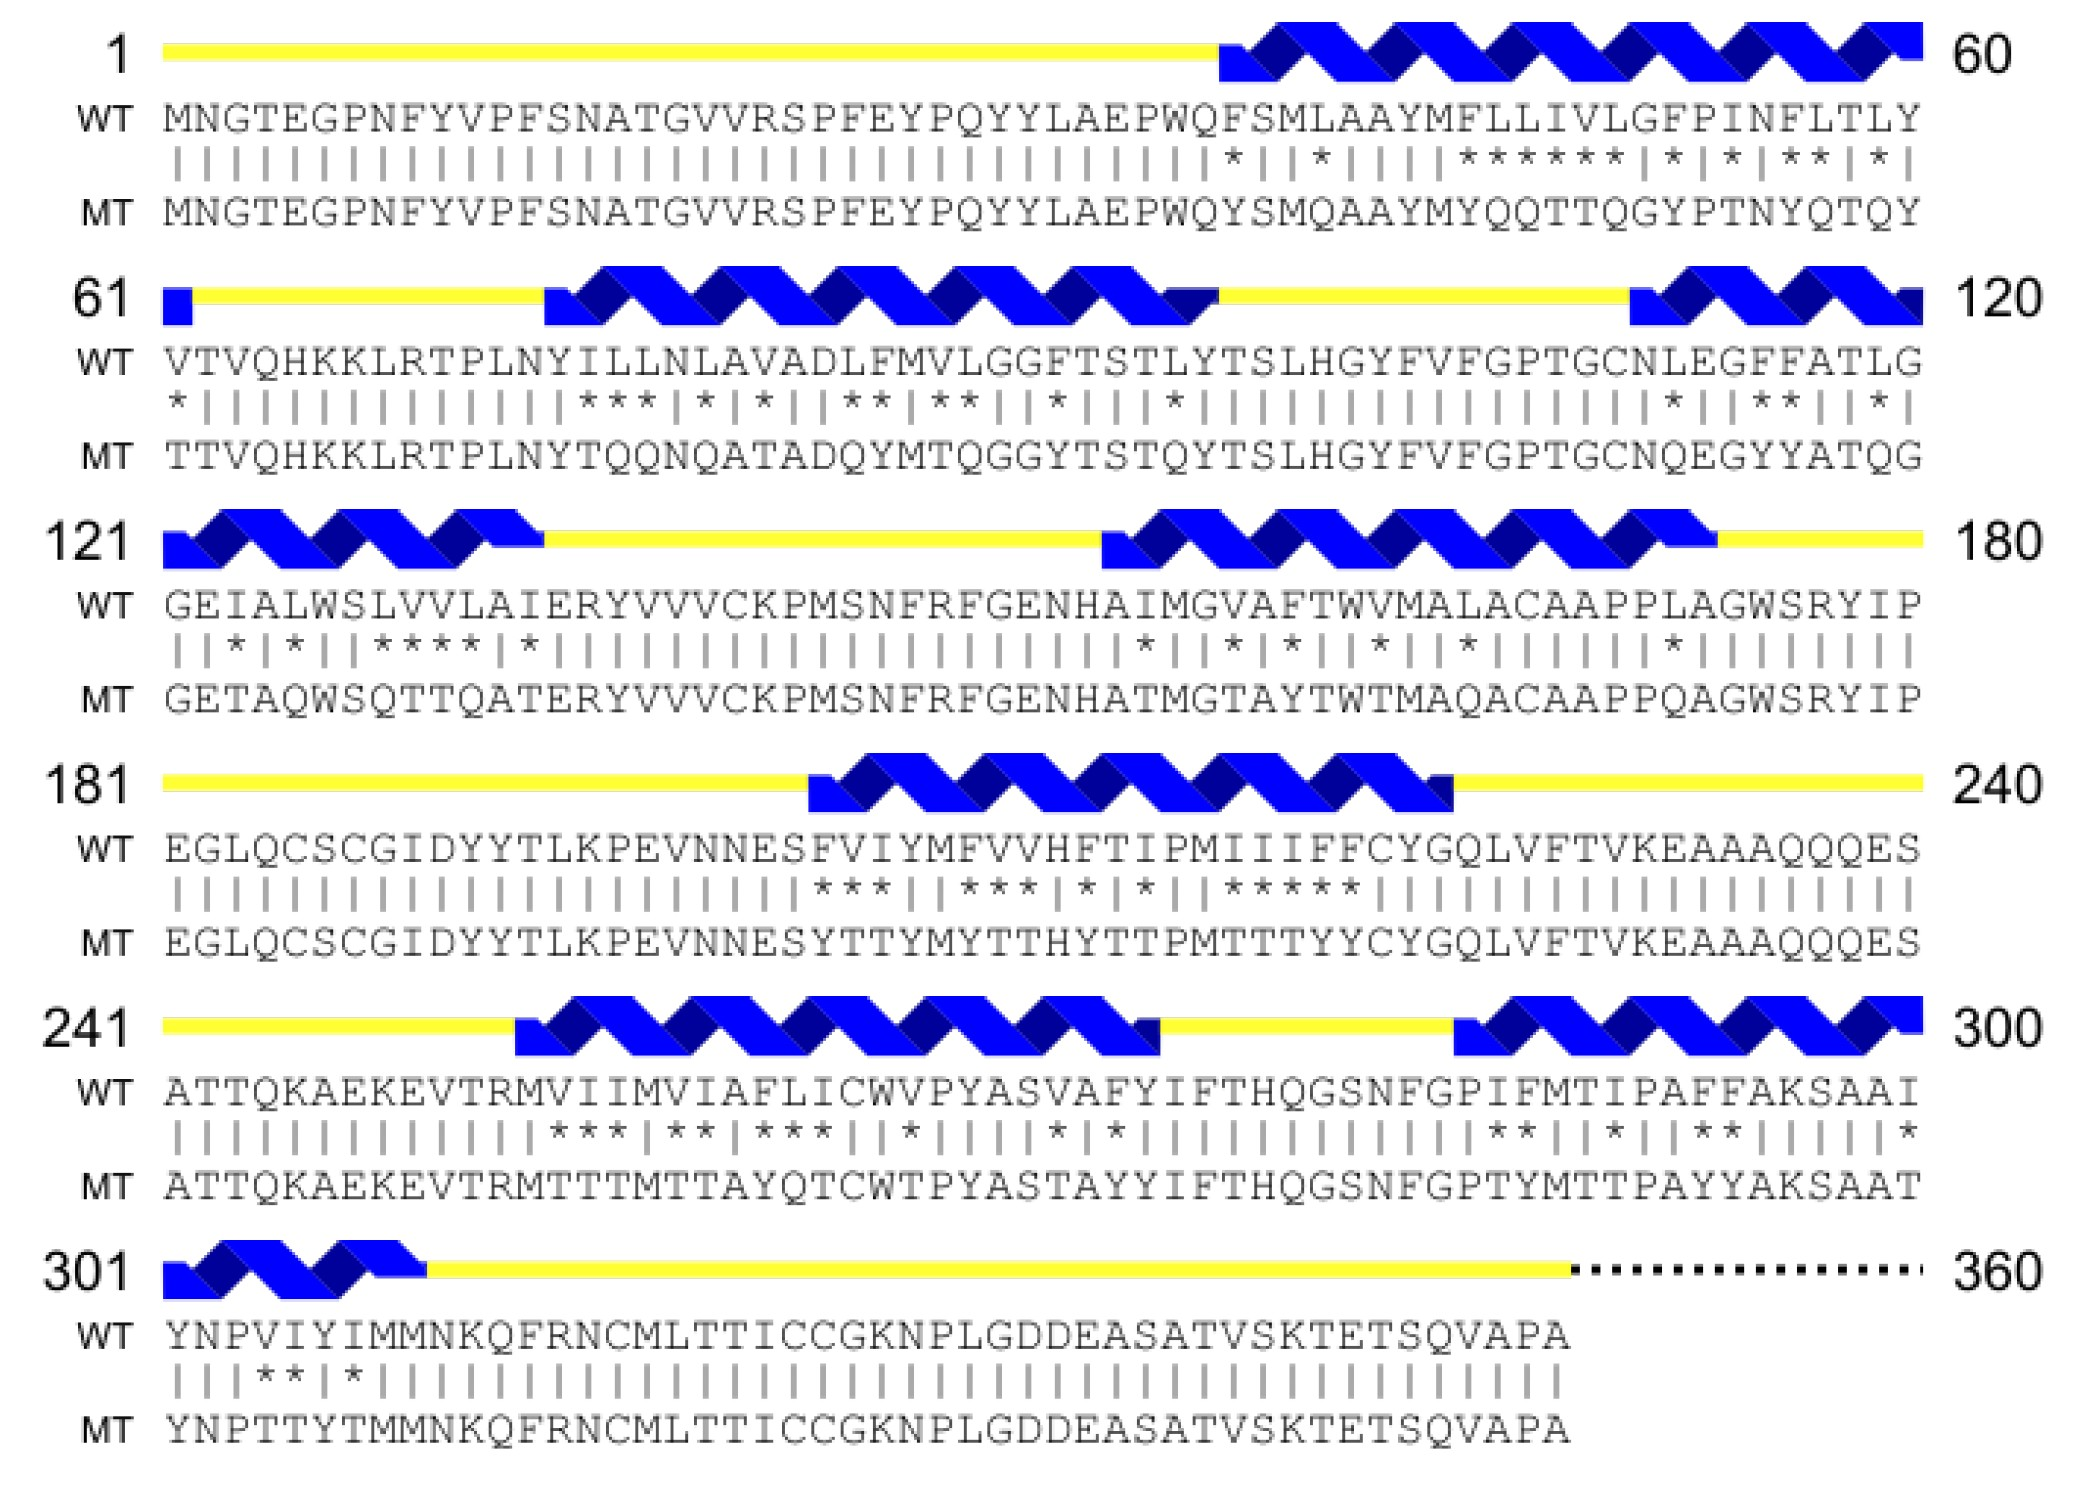
\includegraphics[width=\linewidth]{SuppFigures/opn2.jpg}
\end{figure}

\newpage
\begin{figure}[H]
    \textbf{e)} OPN3 \textit{vs} OPN3$^{\textrm{QTY}}$ \\
    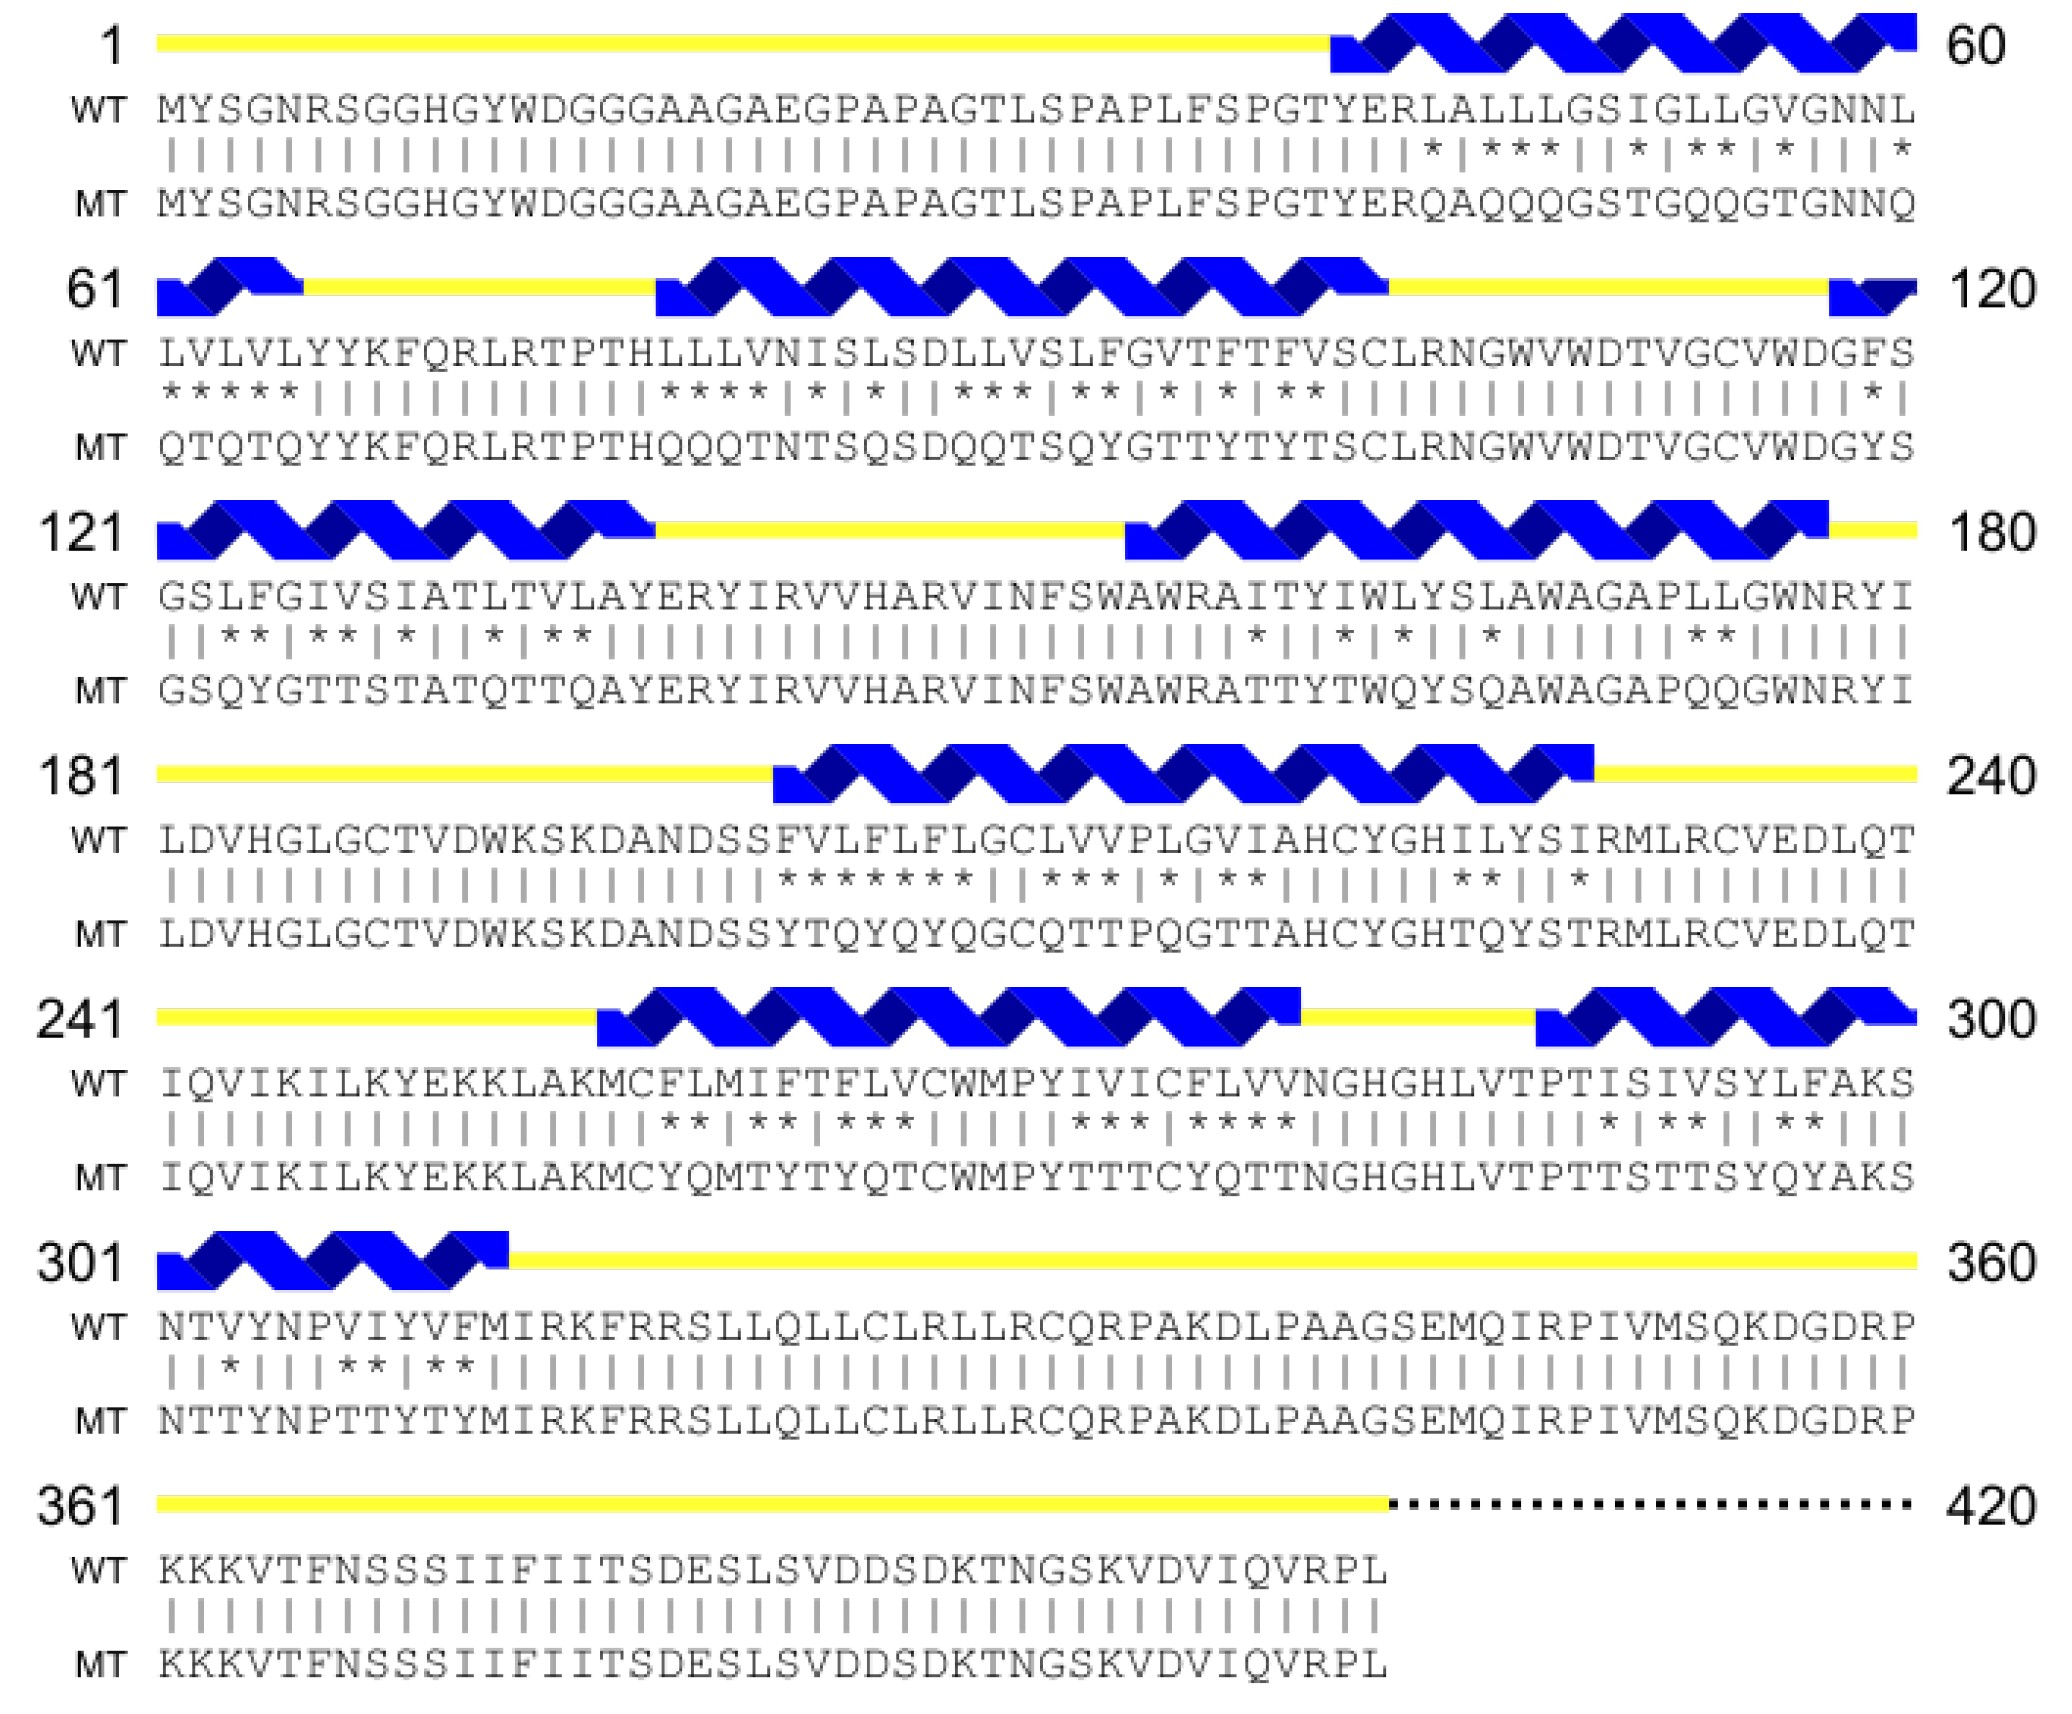
\includegraphics[width=\linewidth]{SuppFigures/opn3.jpg}
\end{figure}

\newpage
\begin{figure}[H]
    \textbf{f)} OPN4 \textit{vs} OPN4$^{\textrm{QTY}}$ \\
    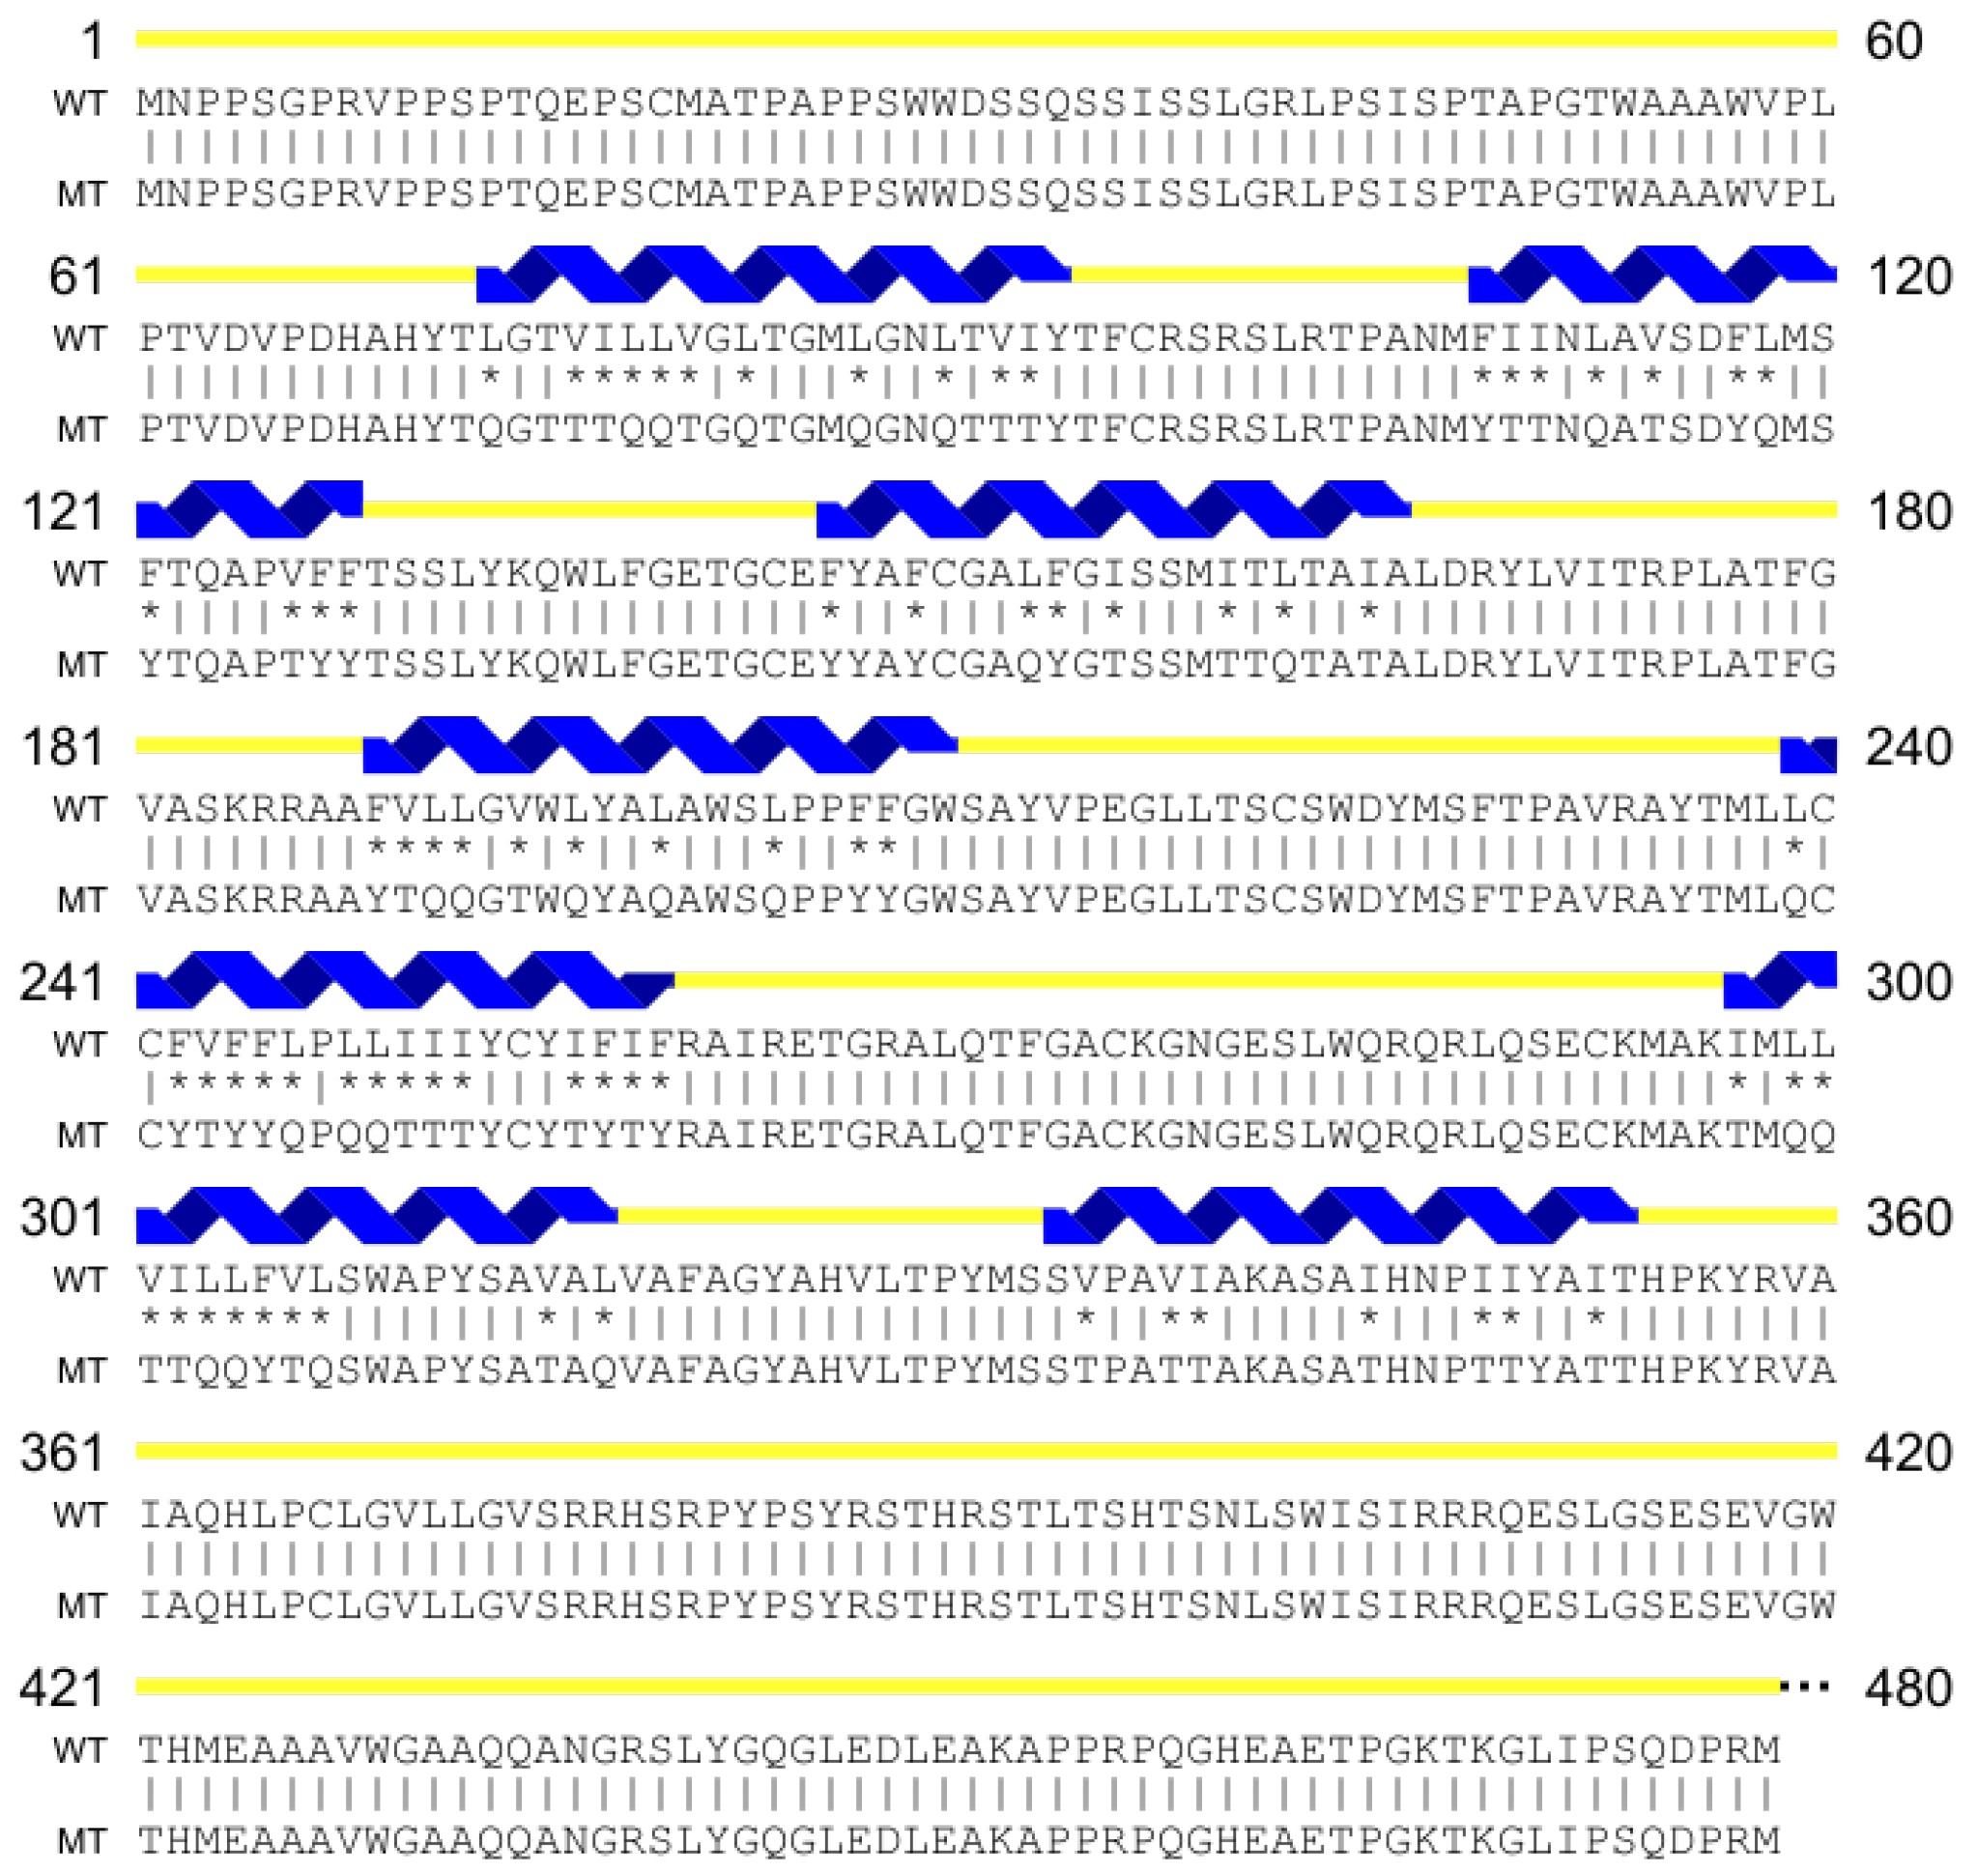
\includegraphics[width=\linewidth]{SuppFigures/opn4.jpg}
\end{figure}

\newpage
\begin{figure}[H]
    \textbf{g)} OPN5 \textit{vs} OPN5$^{\textrm{QTY}}$ \\
    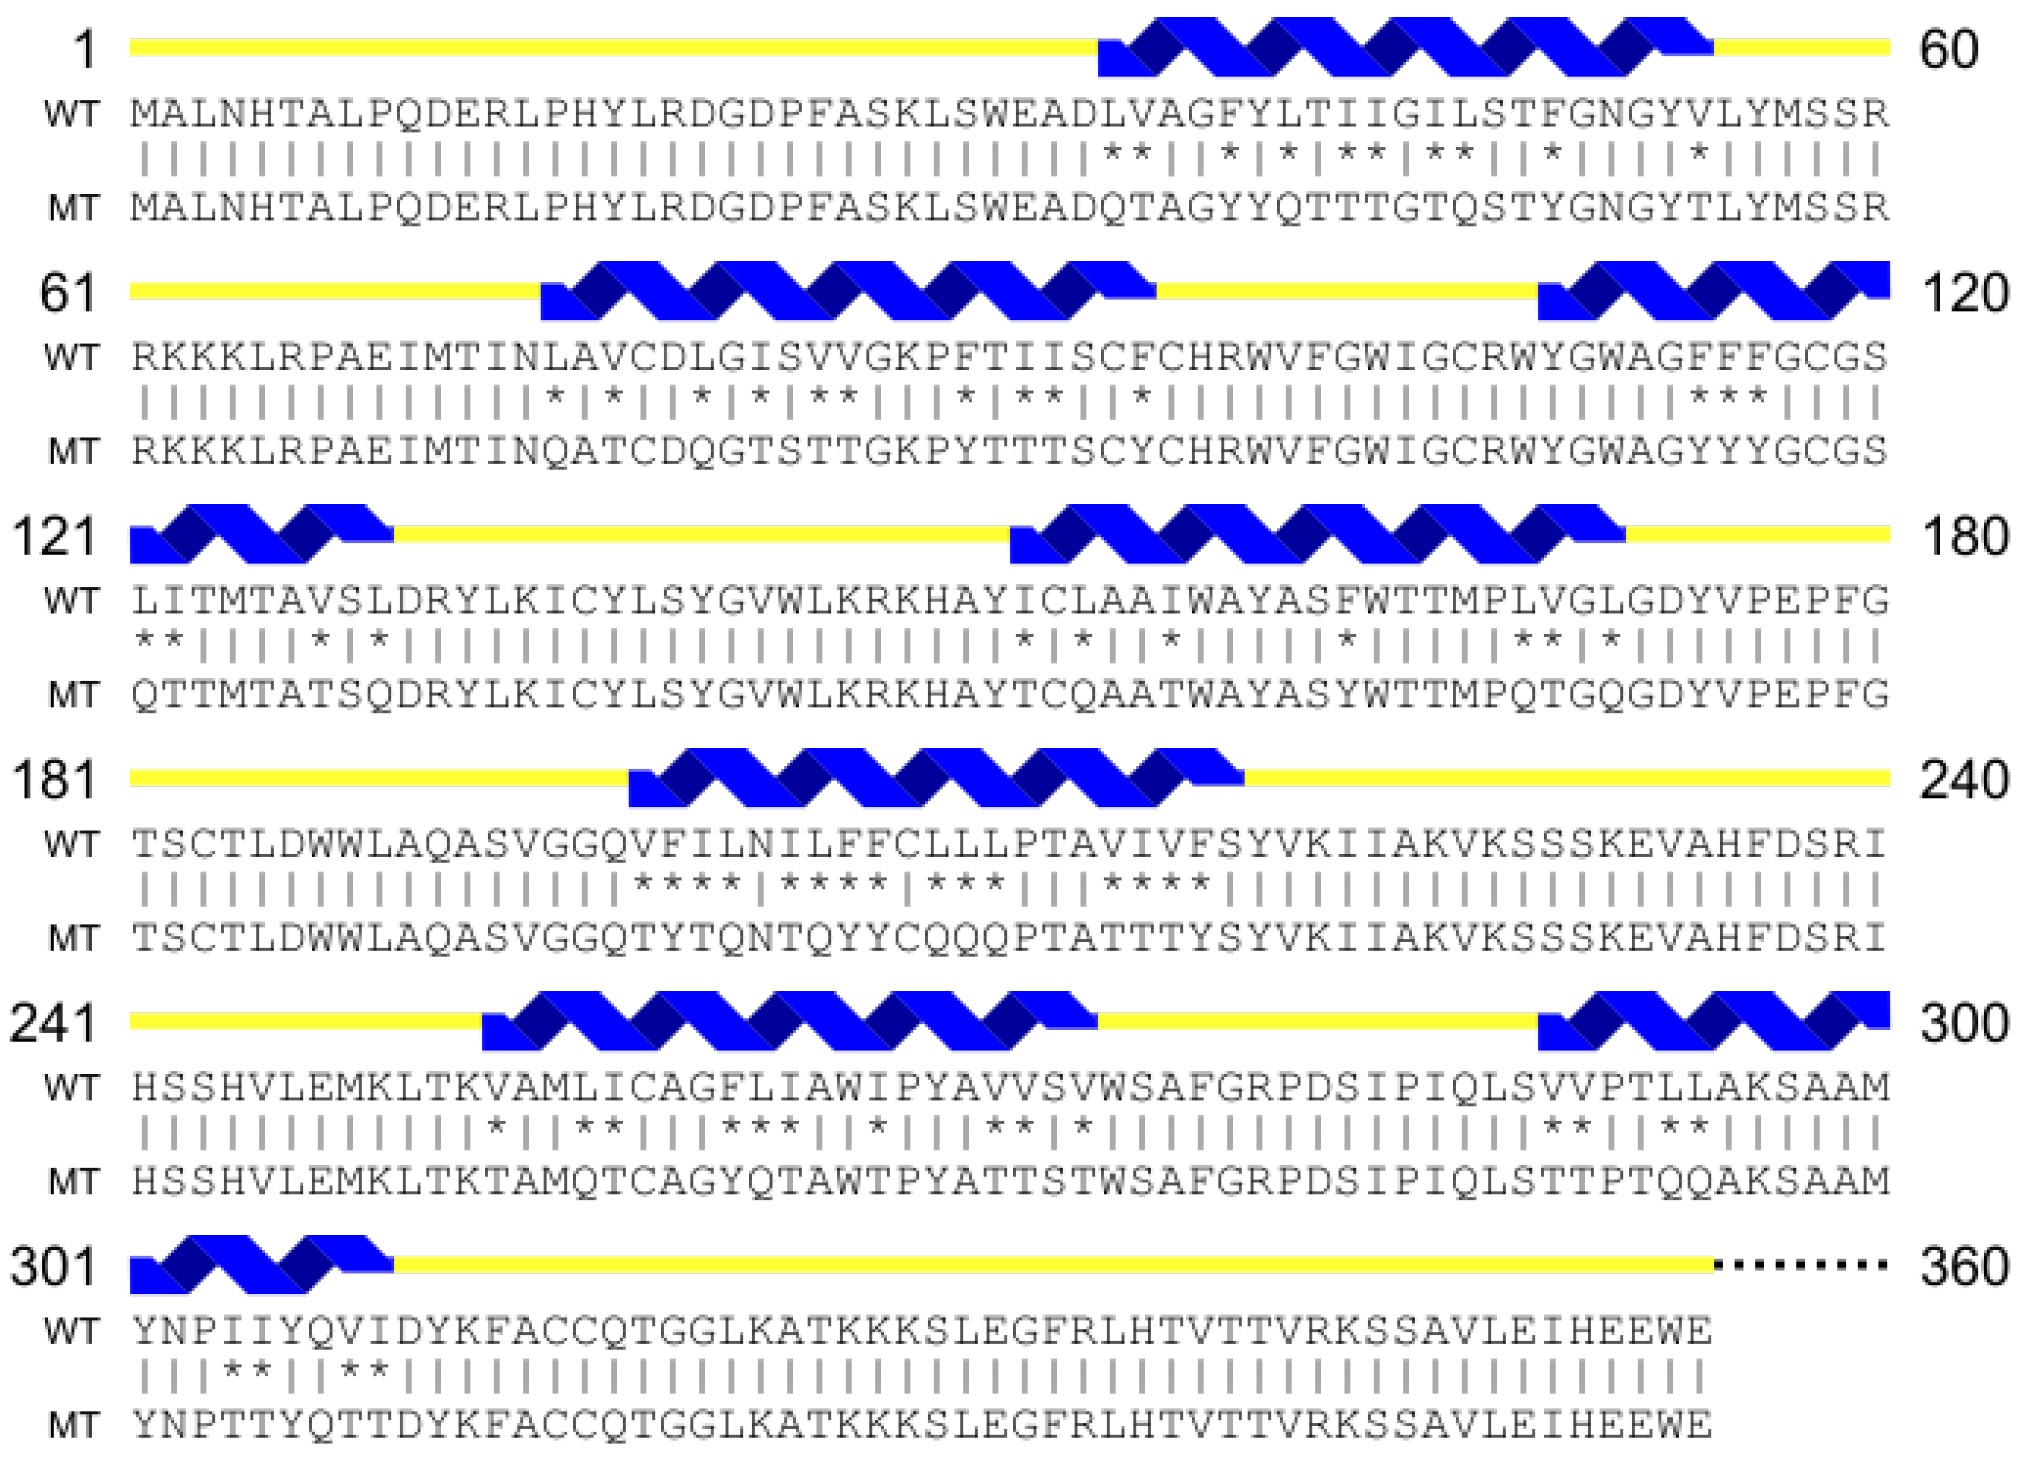
\includegraphics[width=\linewidth]{SuppFigures/opn5.jpg}
\end{figure}

\newpage
\begin{figure}[H]
    \textbf{h)} RGR \textit{vs} RGR$^{\textrm{QTY}}$ \\
    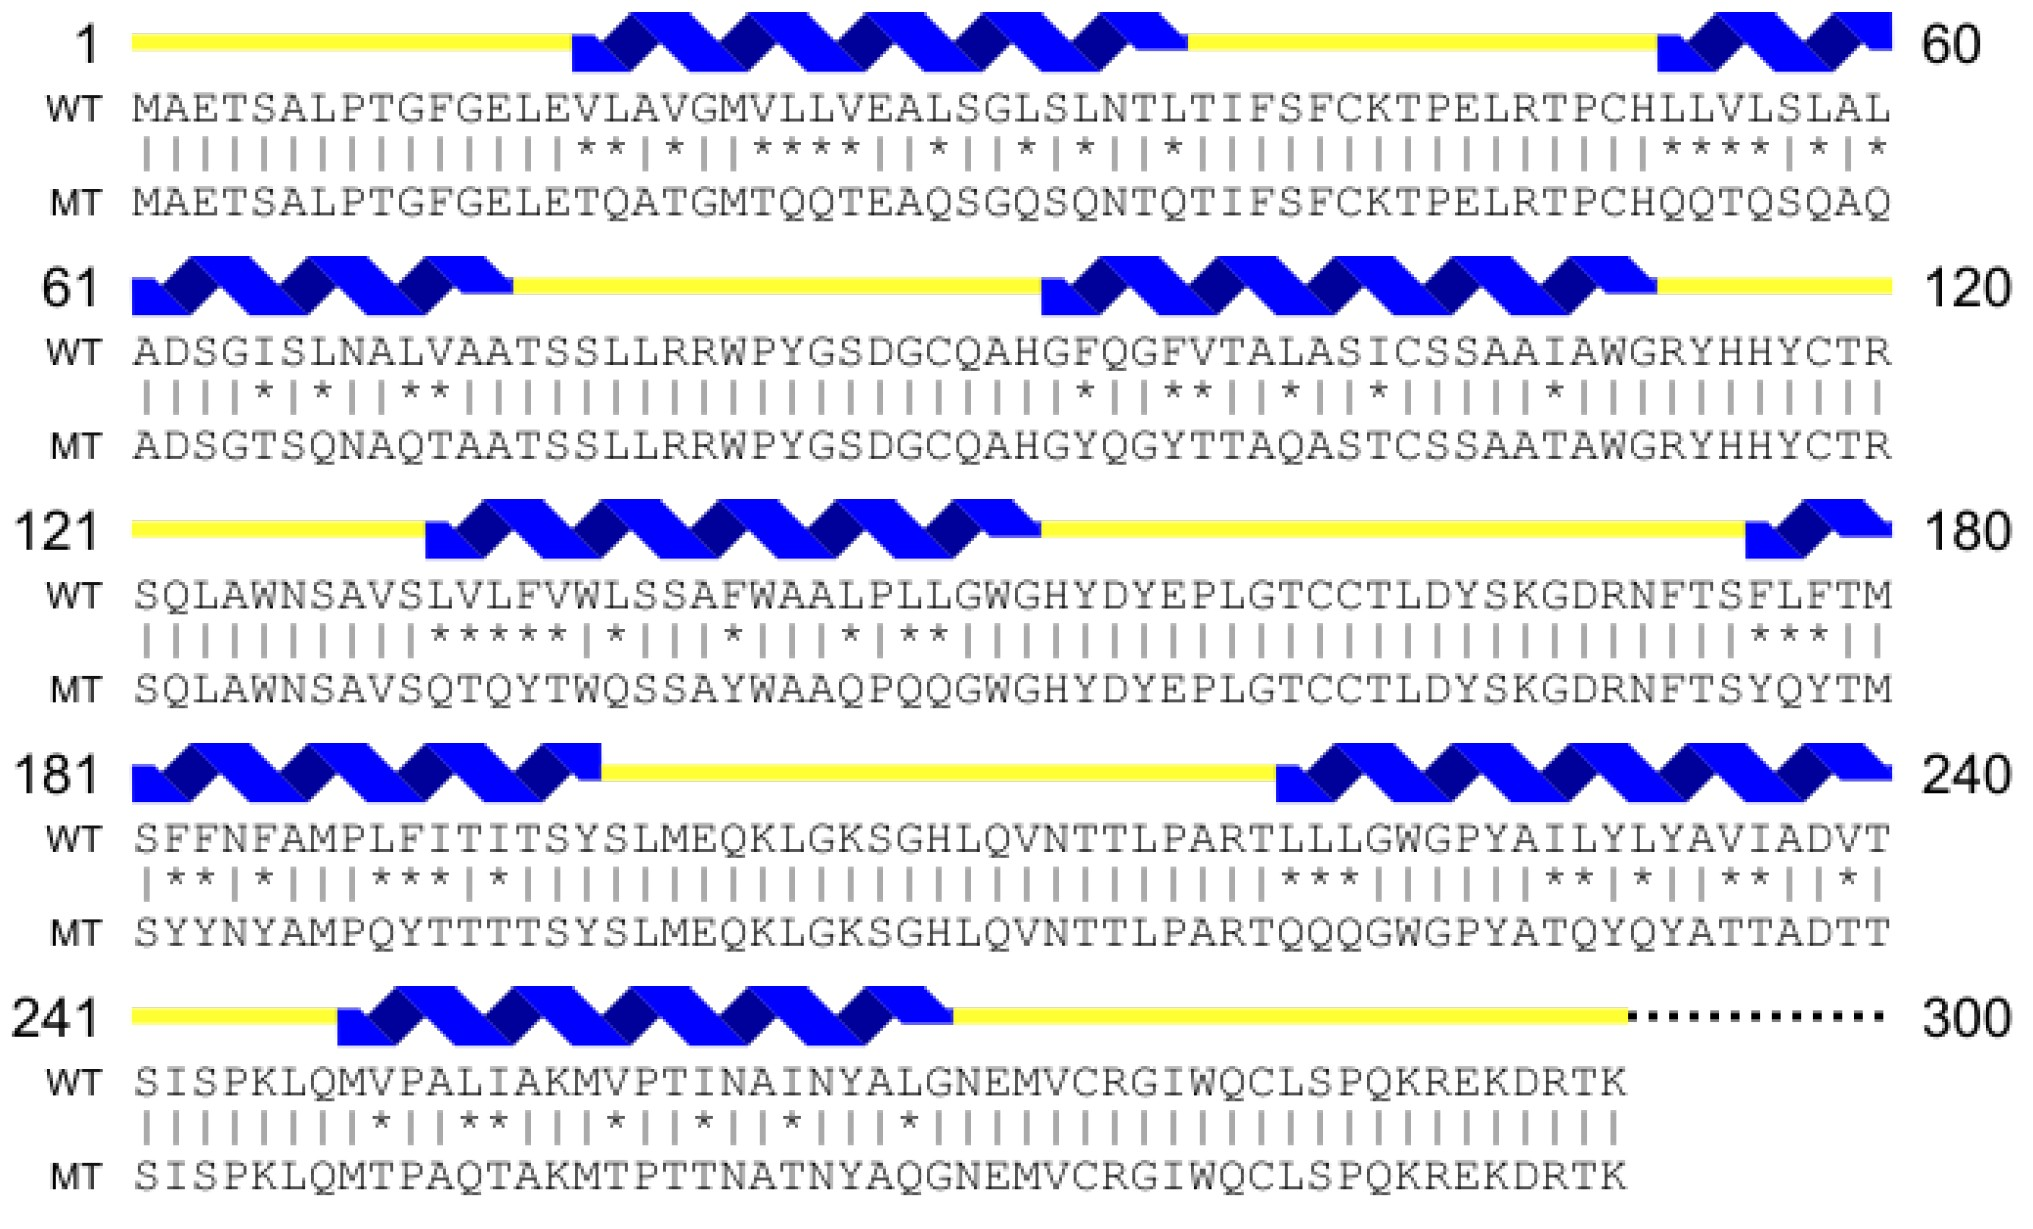
\includegraphics[width=\linewidth]{SuppFigures/rgr.jpg}
\end{figure}

\newpage
\begin{figure}[H]
    \textbf{i)} RRH \textit{vs} RRH$^{\textrm{QTY}}$ \\
    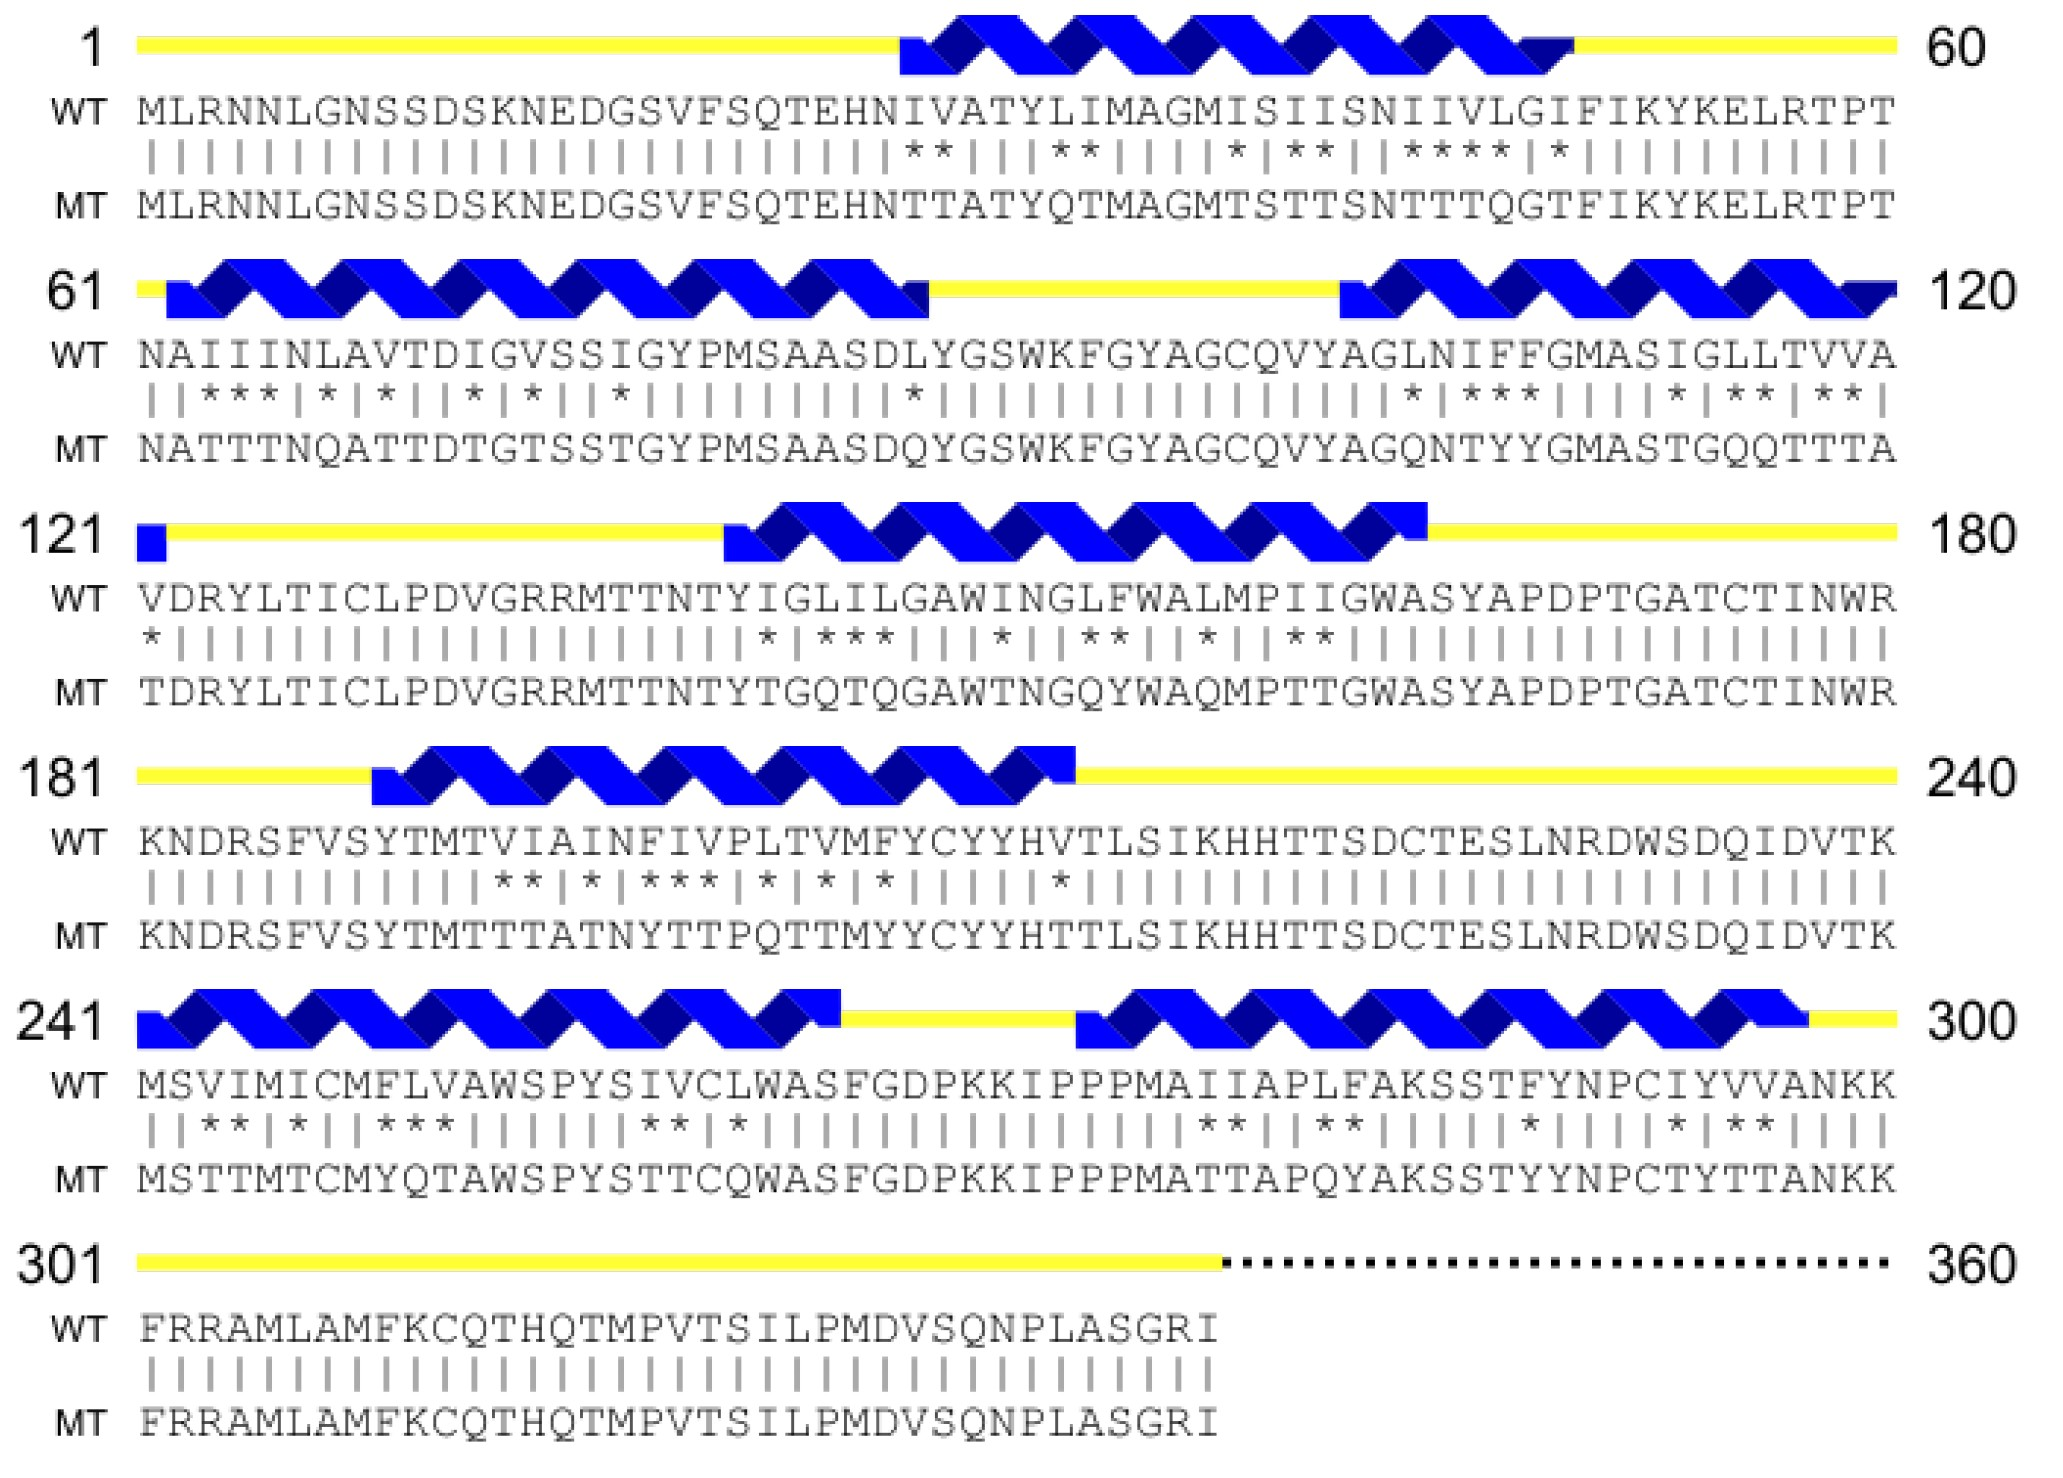
\includegraphics[width=\linewidth]{SuppFigures/rrh.jpg}
\end{figure}

\newpage
\begin{figure}[H]
    \textbf{j)} BACR \textit{vs} BACR$^{\textrm{QTY}}$ \\
    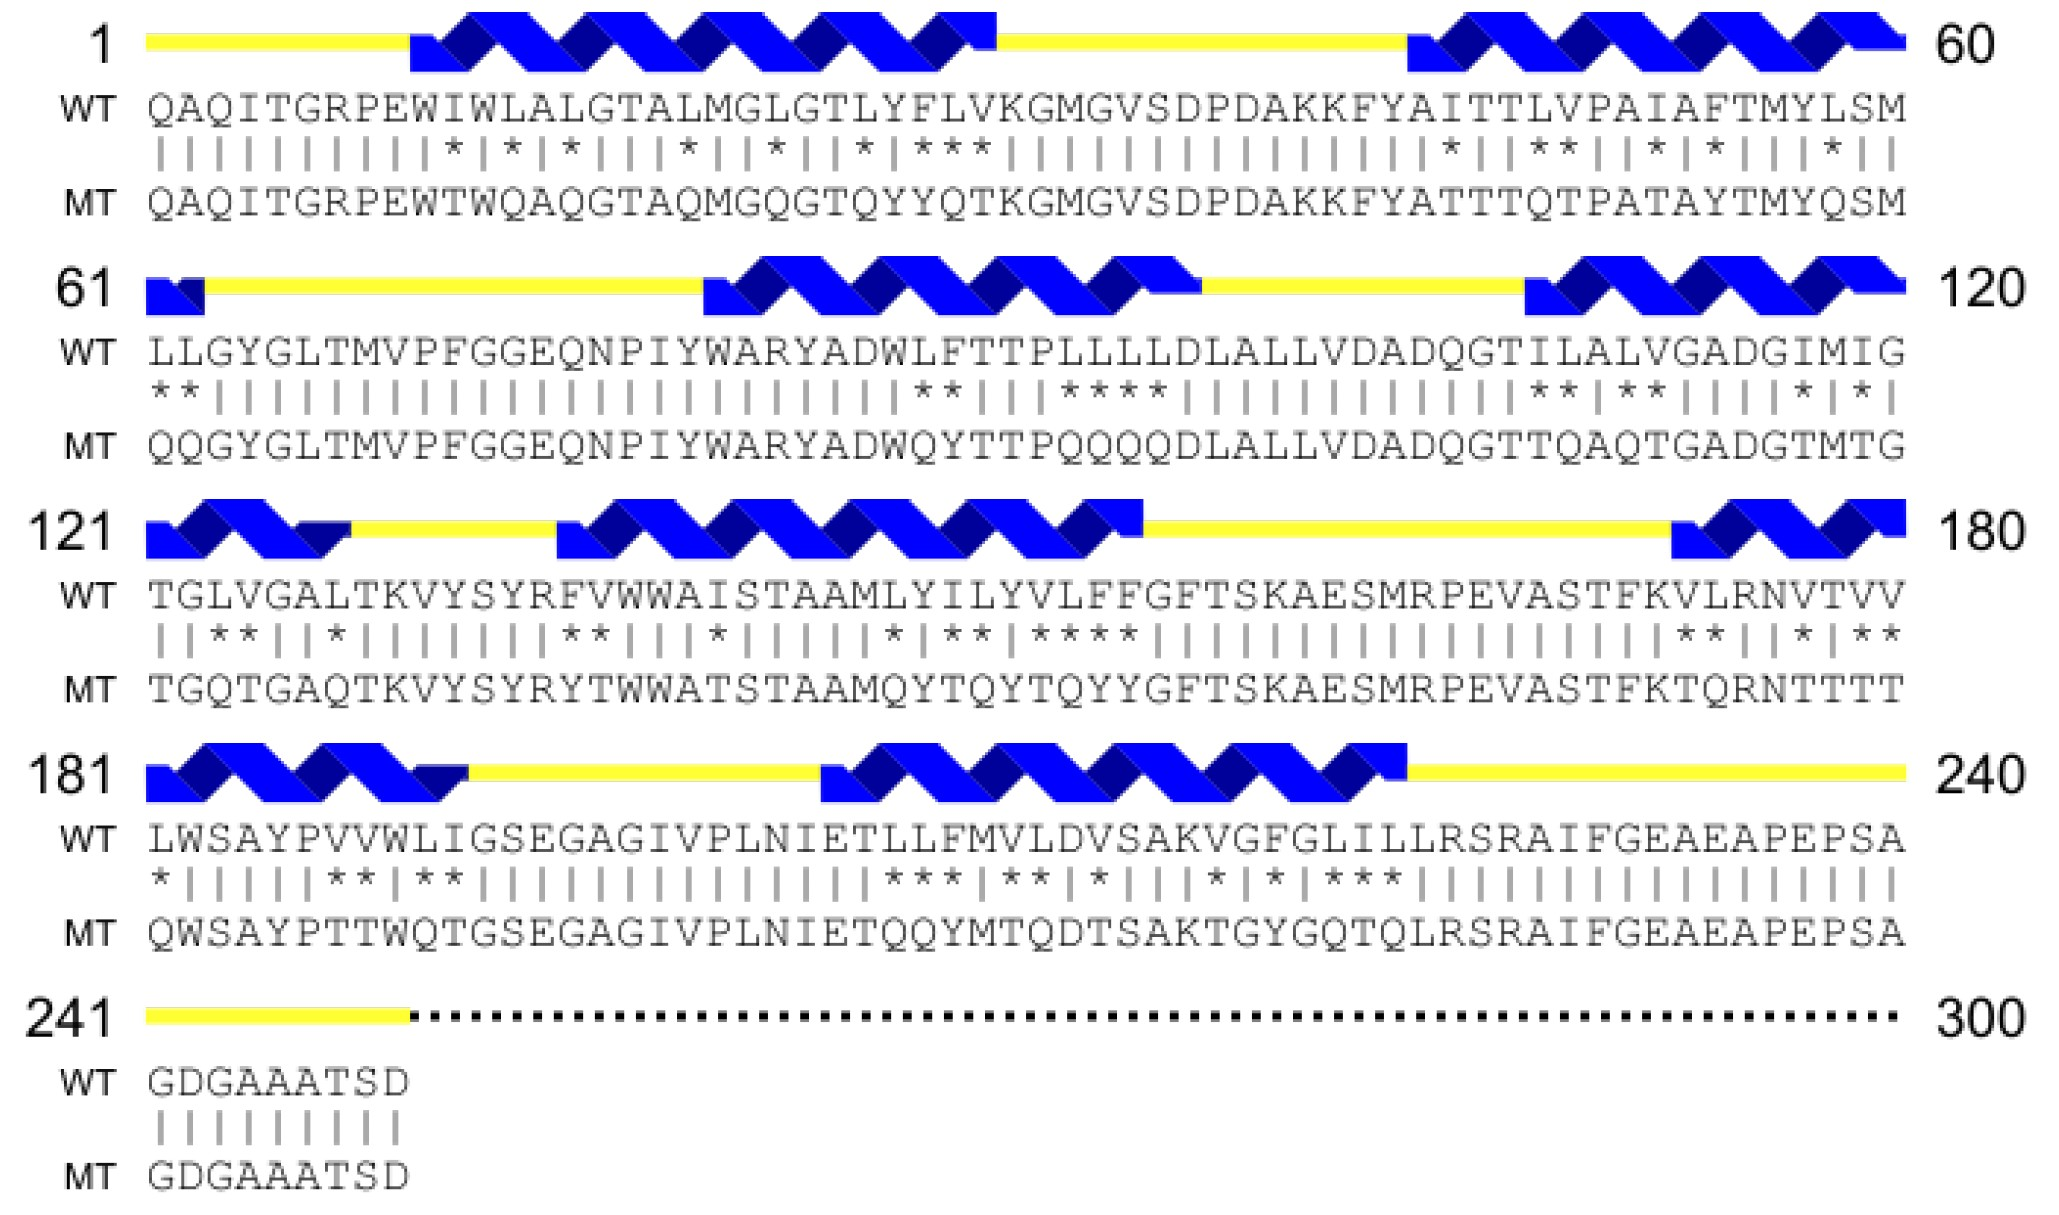
\includegraphics[width=\linewidth]{SuppFigures/bacr.jpg}
\end{figure}

\newpage
\begin{figure}[H]
    \textbf{k)} BACH \textit{vs} BACH$^{\textrm{QTY}}$ \\
    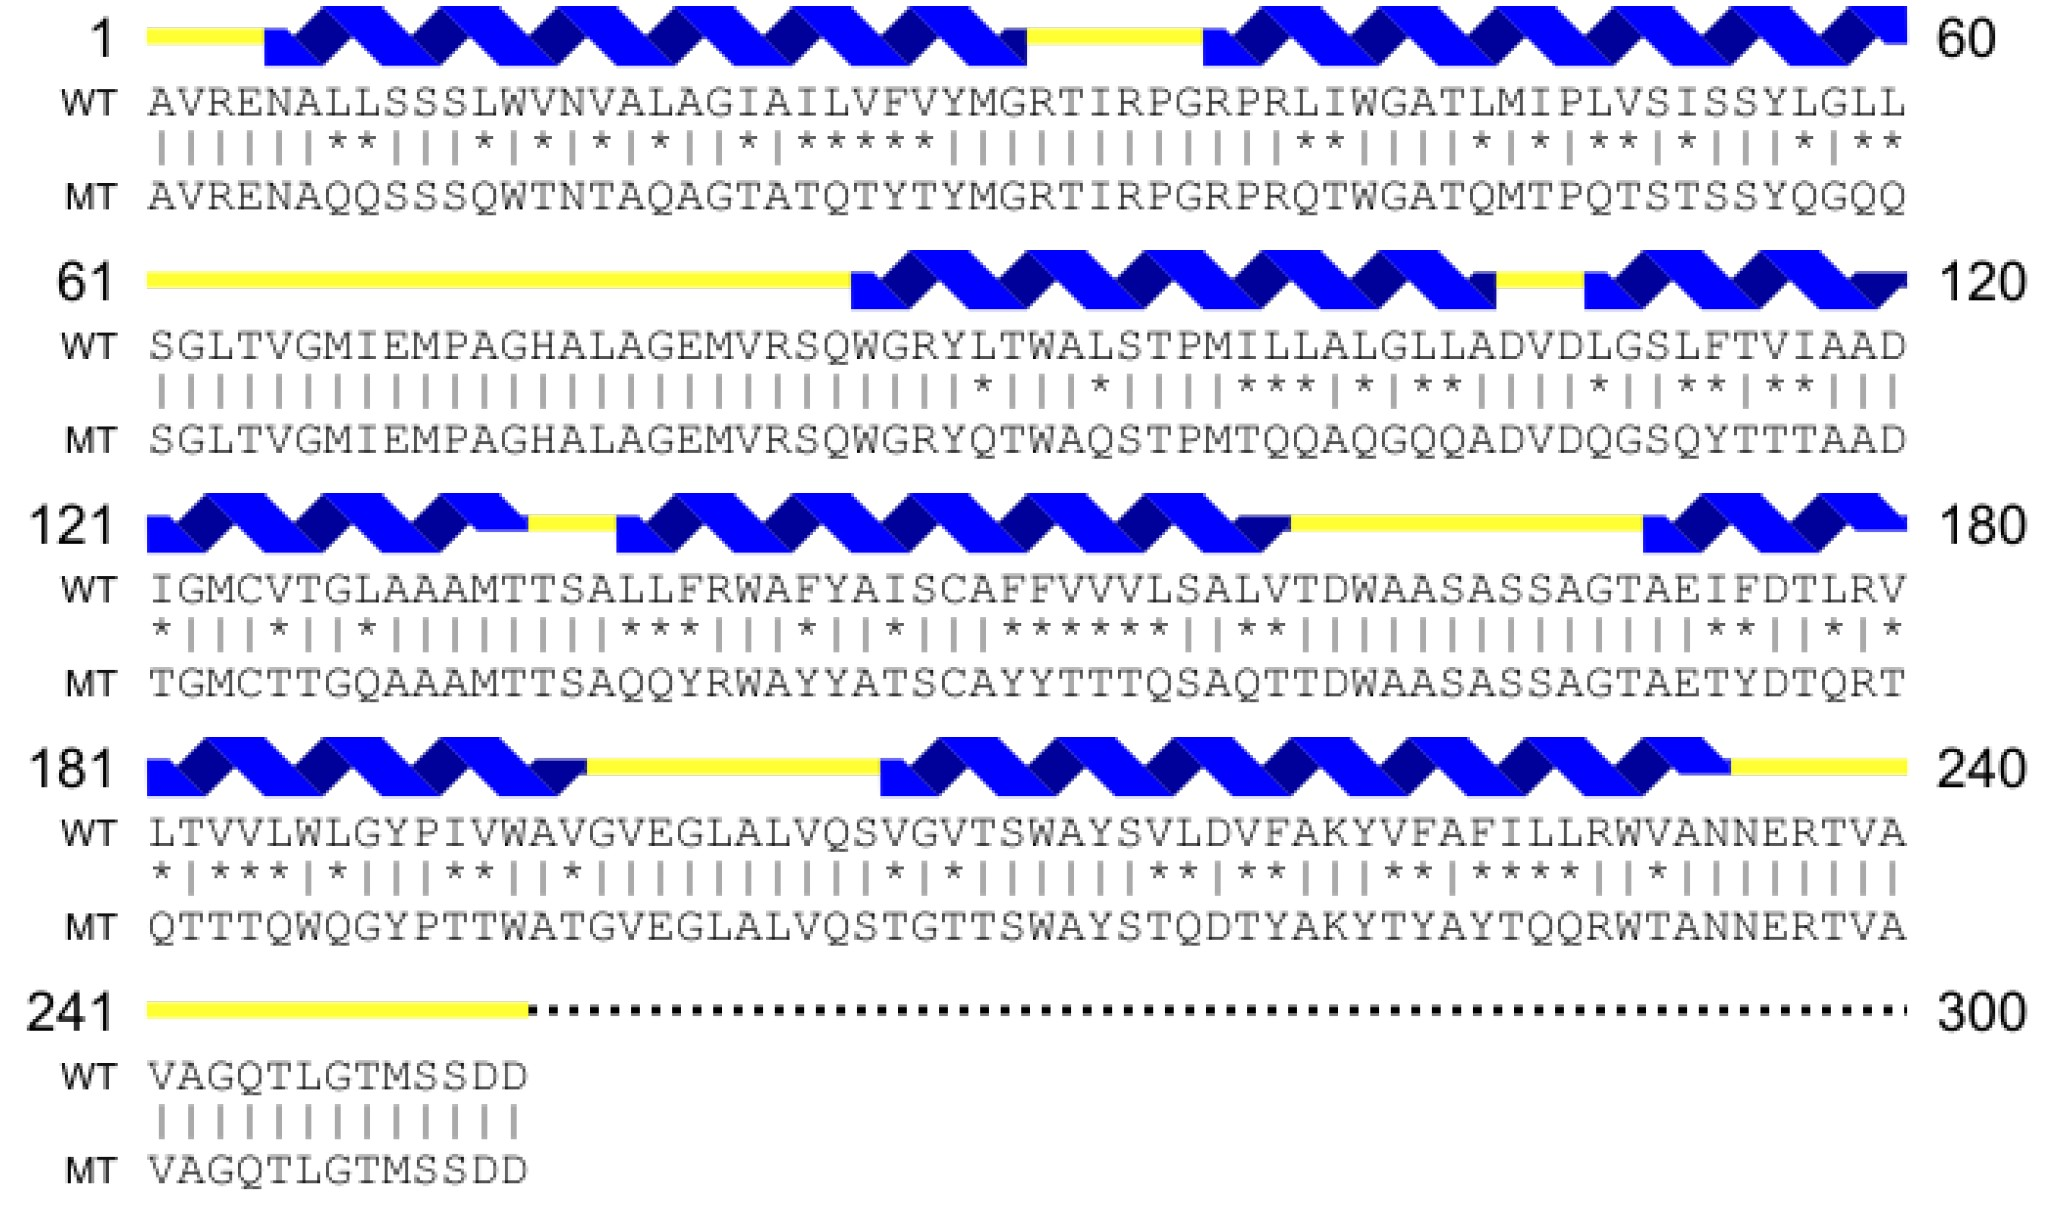
\includegraphics[width=\linewidth]{SuppFigures/bach.jpg}
\end{figure}

\newpage
\begin{figure}[H]
    \textbf{l)} ChR2 \textit{vs} ChR2$^{\textrm{QTY}}$ \\
    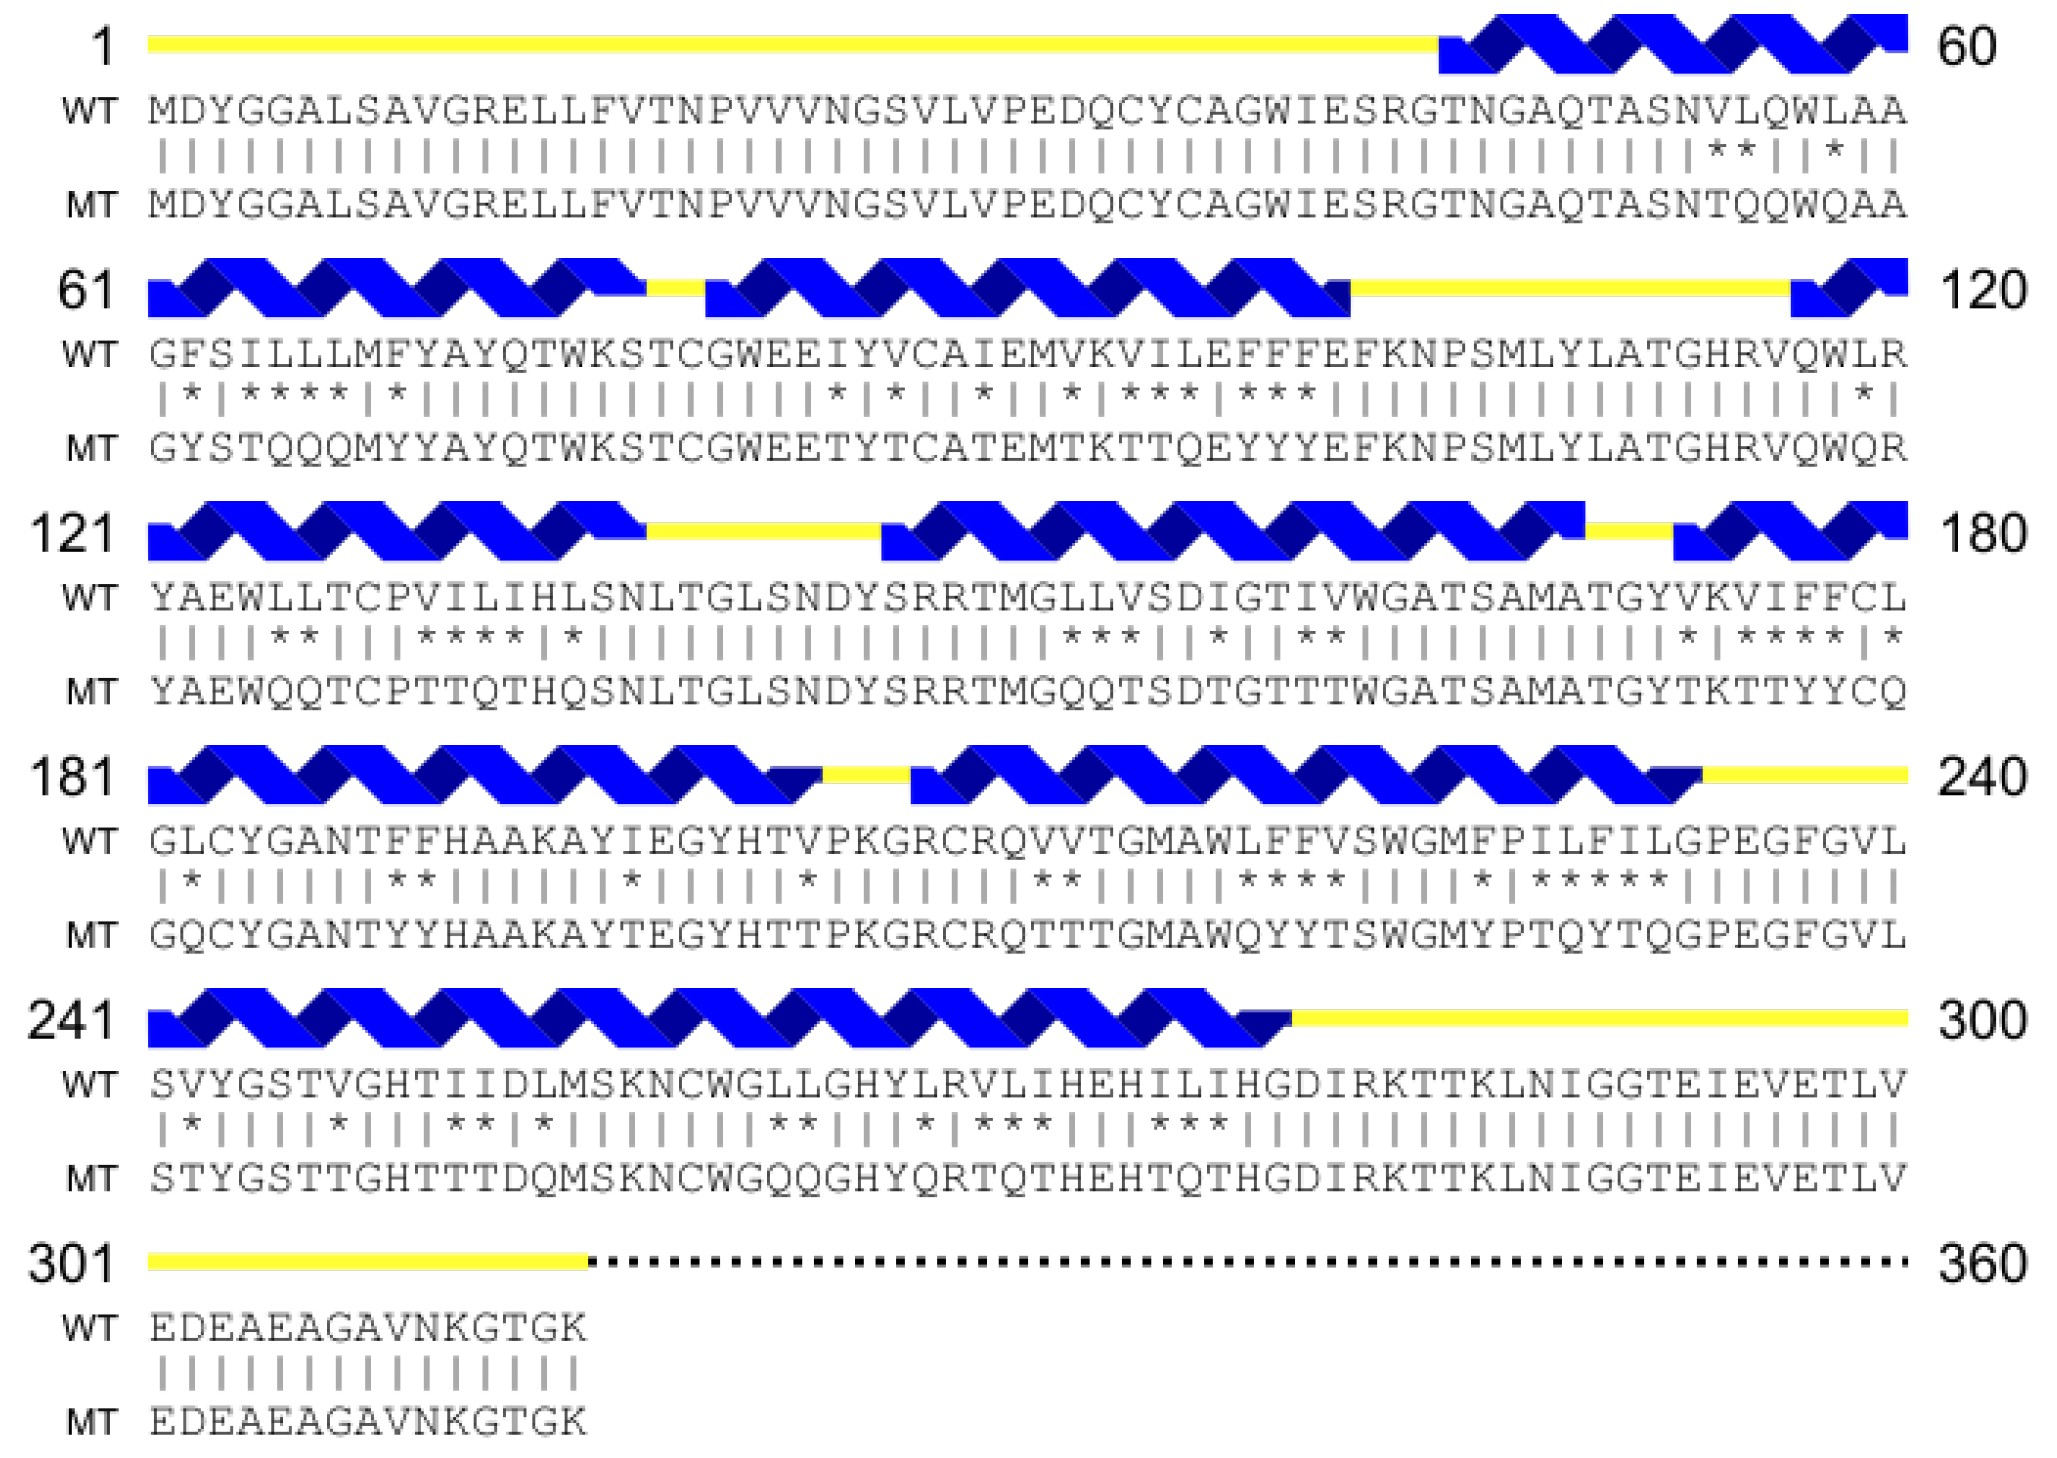
\includegraphics[width=\linewidth]{SuppFigures/chr2.jpg}
\end{figure}



\begin{figure}[H]
    \caption{\textbf{AlphaFold3 prediction accuracy: plDDT, PAE, ipTM, and pTM scores.} \\
    The scores are displayed for the following proteins: 
    \textbf{a)} OPN1MW$^{\textrm{QTY}}$,
    \textbf{b)} OPN1LW$^{\textrm{QTY}}$,
    \textbf{c)} OPN1SW$^{\textrm{QTY}}$,
    \textbf{d)} OPN2$^{\textrm{QTY}}$,
    \textbf{e)} OPN3$^{\textrm{QTY}}$,
    \textbf{f)} OPN4$^{\textrm{QTY}}$,
    \textbf{g)} OPN5$^{\textrm{QTY}}$,
    \textbf{h)} RGR$^{\textrm{QTY}}$,
    \textbf{i)} RRH$^{\textrm{QTY}}$,
    \textbf{j)} BACR$^{\textrm{QTY}}$ monomer,
    \textbf{k)} BACH$^{\textrm{QTY}}$ monomer,
    \textbf{l)} ChR2$^{\textrm{QTY}}$ monomer,
    \textbf{m)} BACR$^{\textrm{QTY}}$ trimer,
    \textbf{n)} BACH$^{\textrm{QTY}}$ trimer,
    \textbf{o)} ChR2$^{\textrm{QTY}}$ dimer.}
    \textbf{a)} OPN1MW$^{\textrm{QTY}}$ \\
    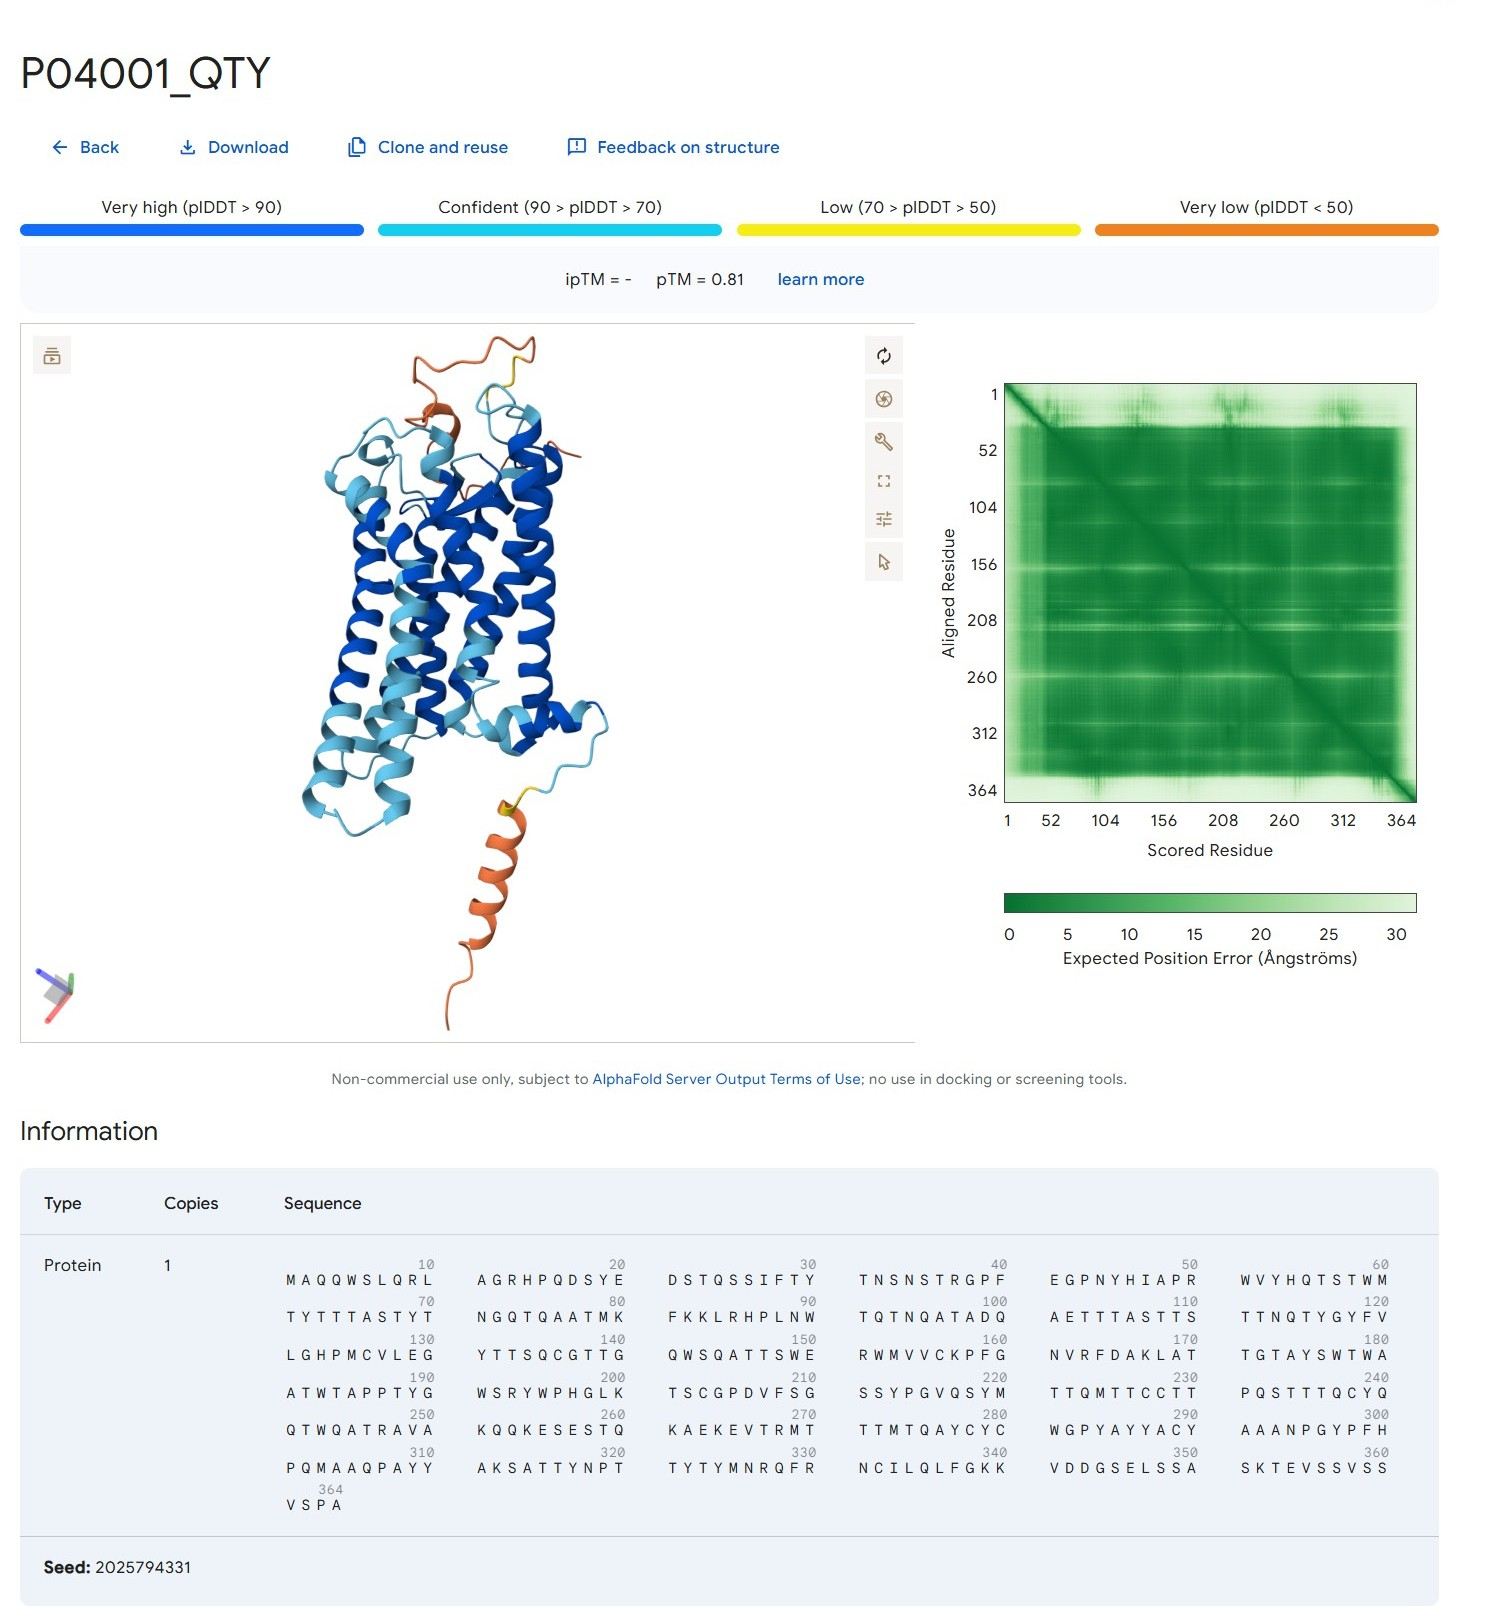
\includegraphics[width=\linewidth]{SuppFigures/af3 opn1mw qty.jpg}
\end{figure}

\newpage
\begin{figure}[H]
    \textbf{b)} OPN1LW$^{\textrm{QTY}}$ \\
    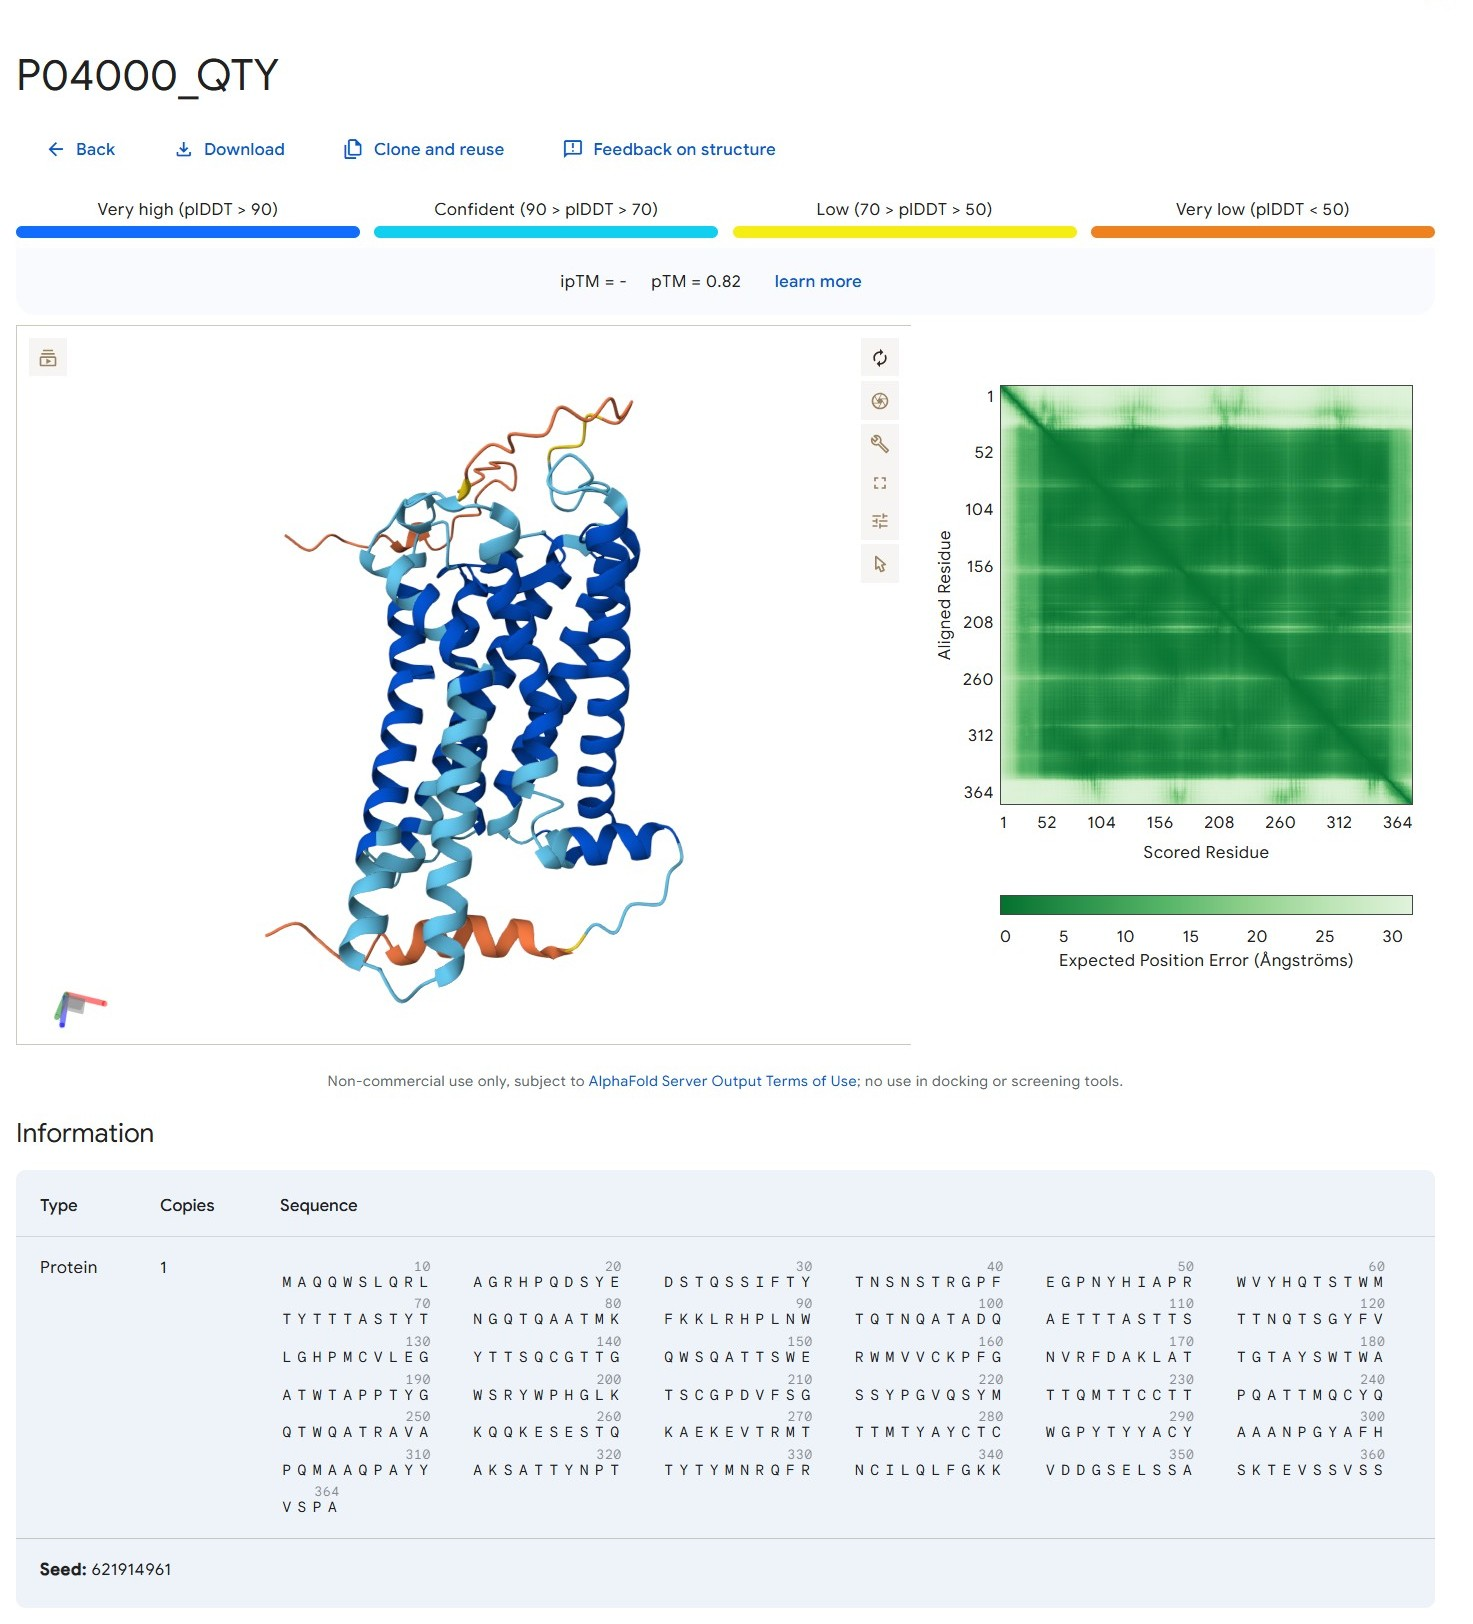
\includegraphics[width=\linewidth]{SuppFigures/af3 opn1lw qty.jpg}
\end{figure}

\newpage
\begin{figure}[H]
    \textbf{c)} OPN1SW$^{\textrm{QTY}}$ \\
    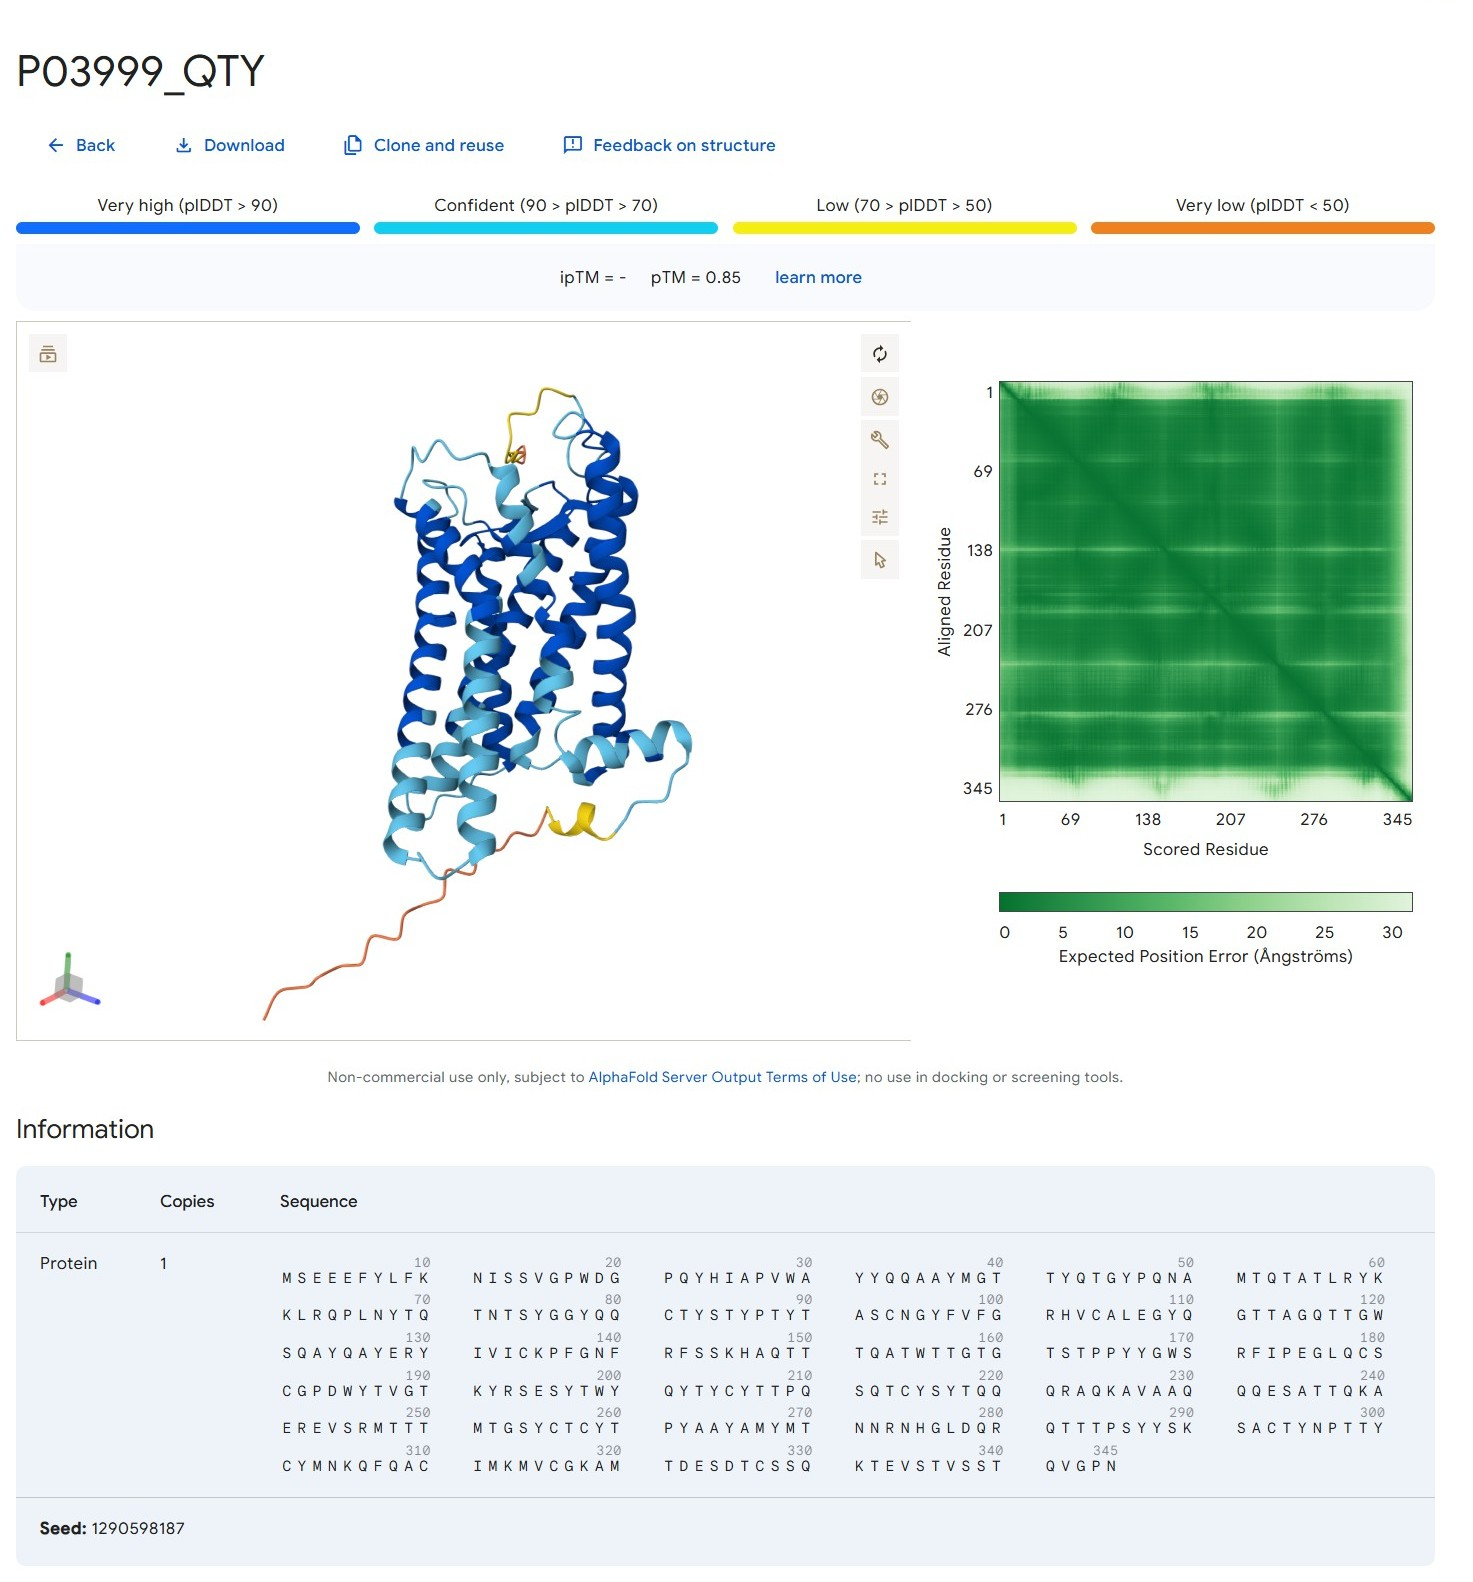
\includegraphics[width=\linewidth]{SuppFigures/af3 opn1sw qty.jpg}
\end{figure}

\newpage
\begin{figure}[H]
    \textbf{d)} OPN2$^{\textrm{QTY}}$ \\
    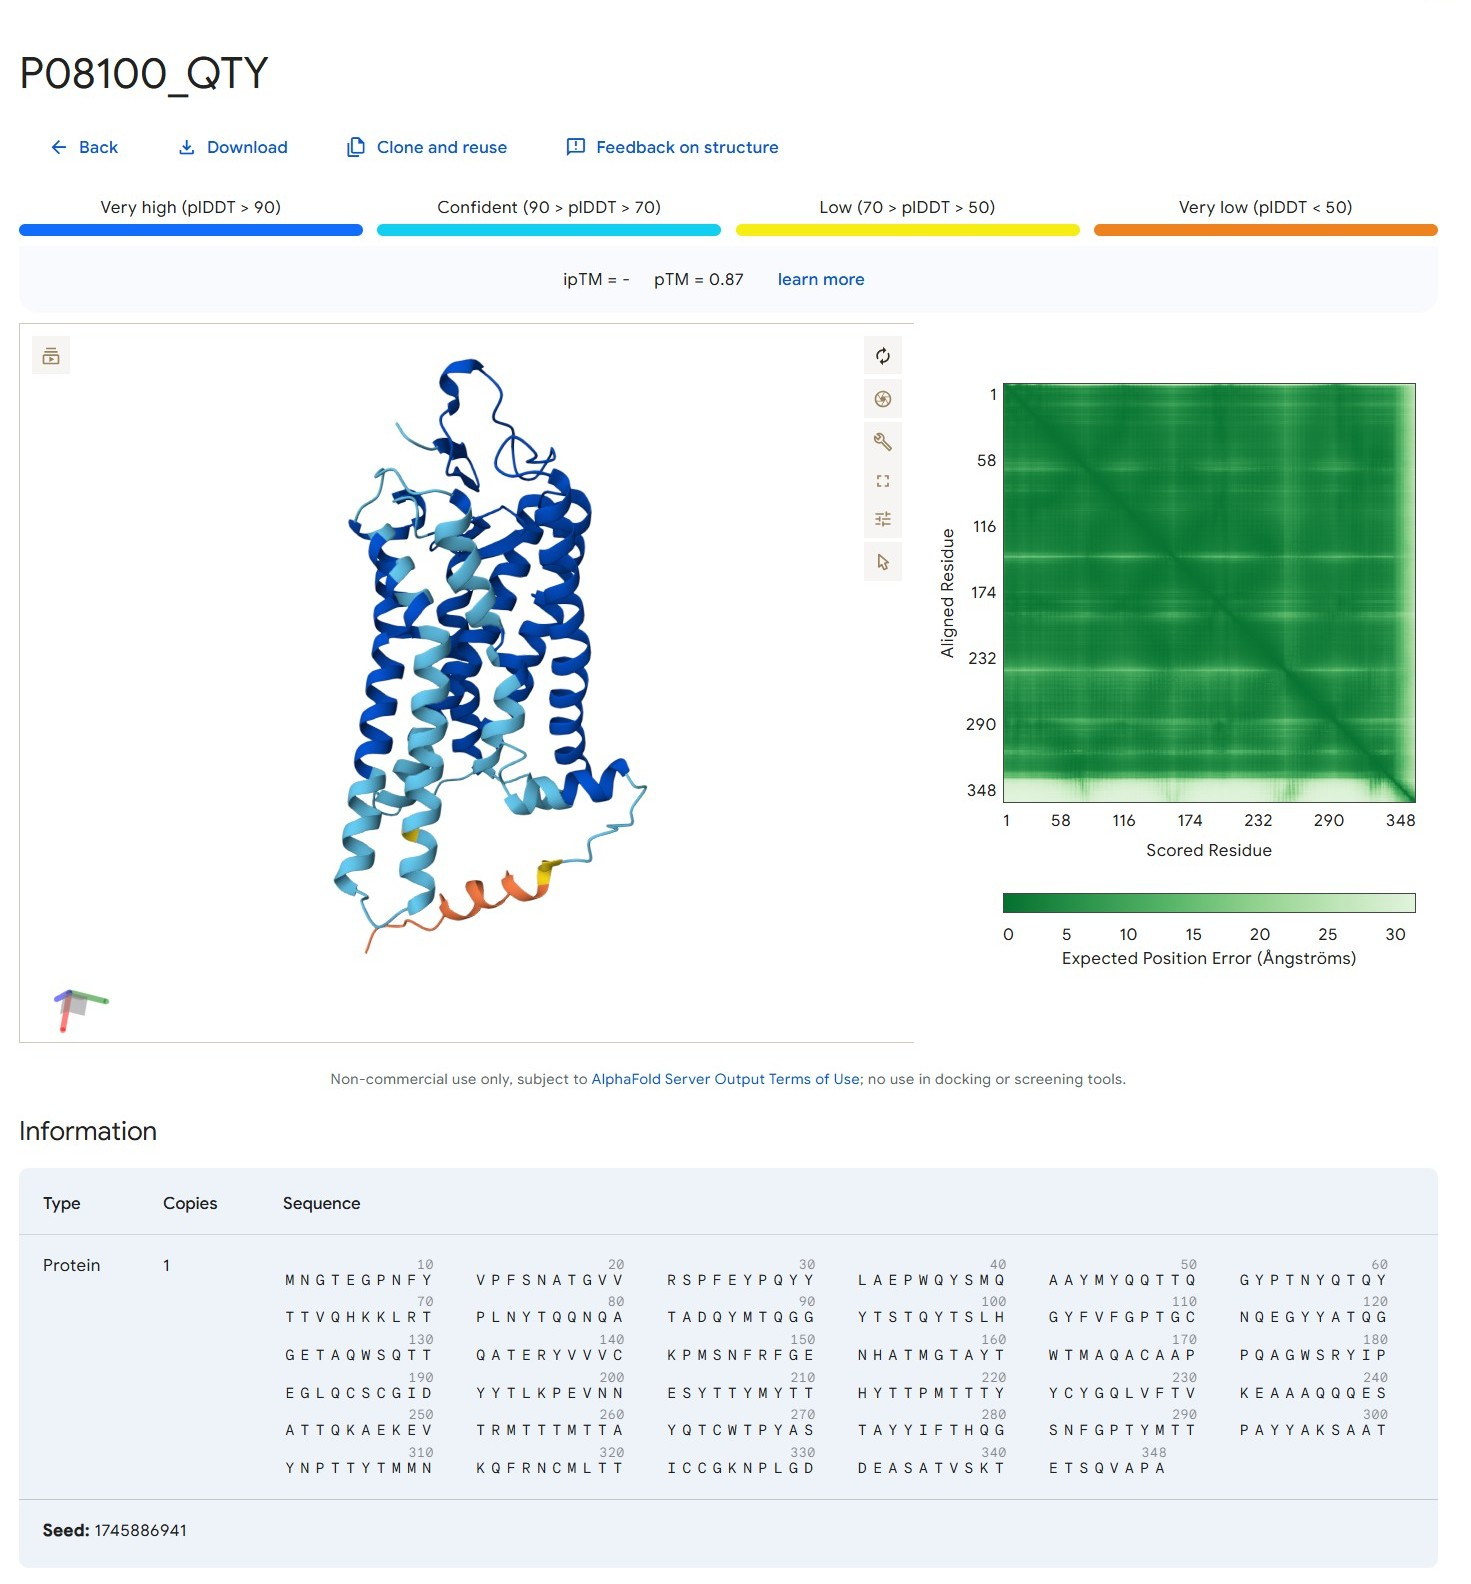
\includegraphics[width=\linewidth]{SuppFigures/af3 opn2 qty.jpg}
\end{figure}

\newpage
\begin{figure}[H]
    \textbf{e)} OPN3$^{\textrm{QTY}}$ \\
    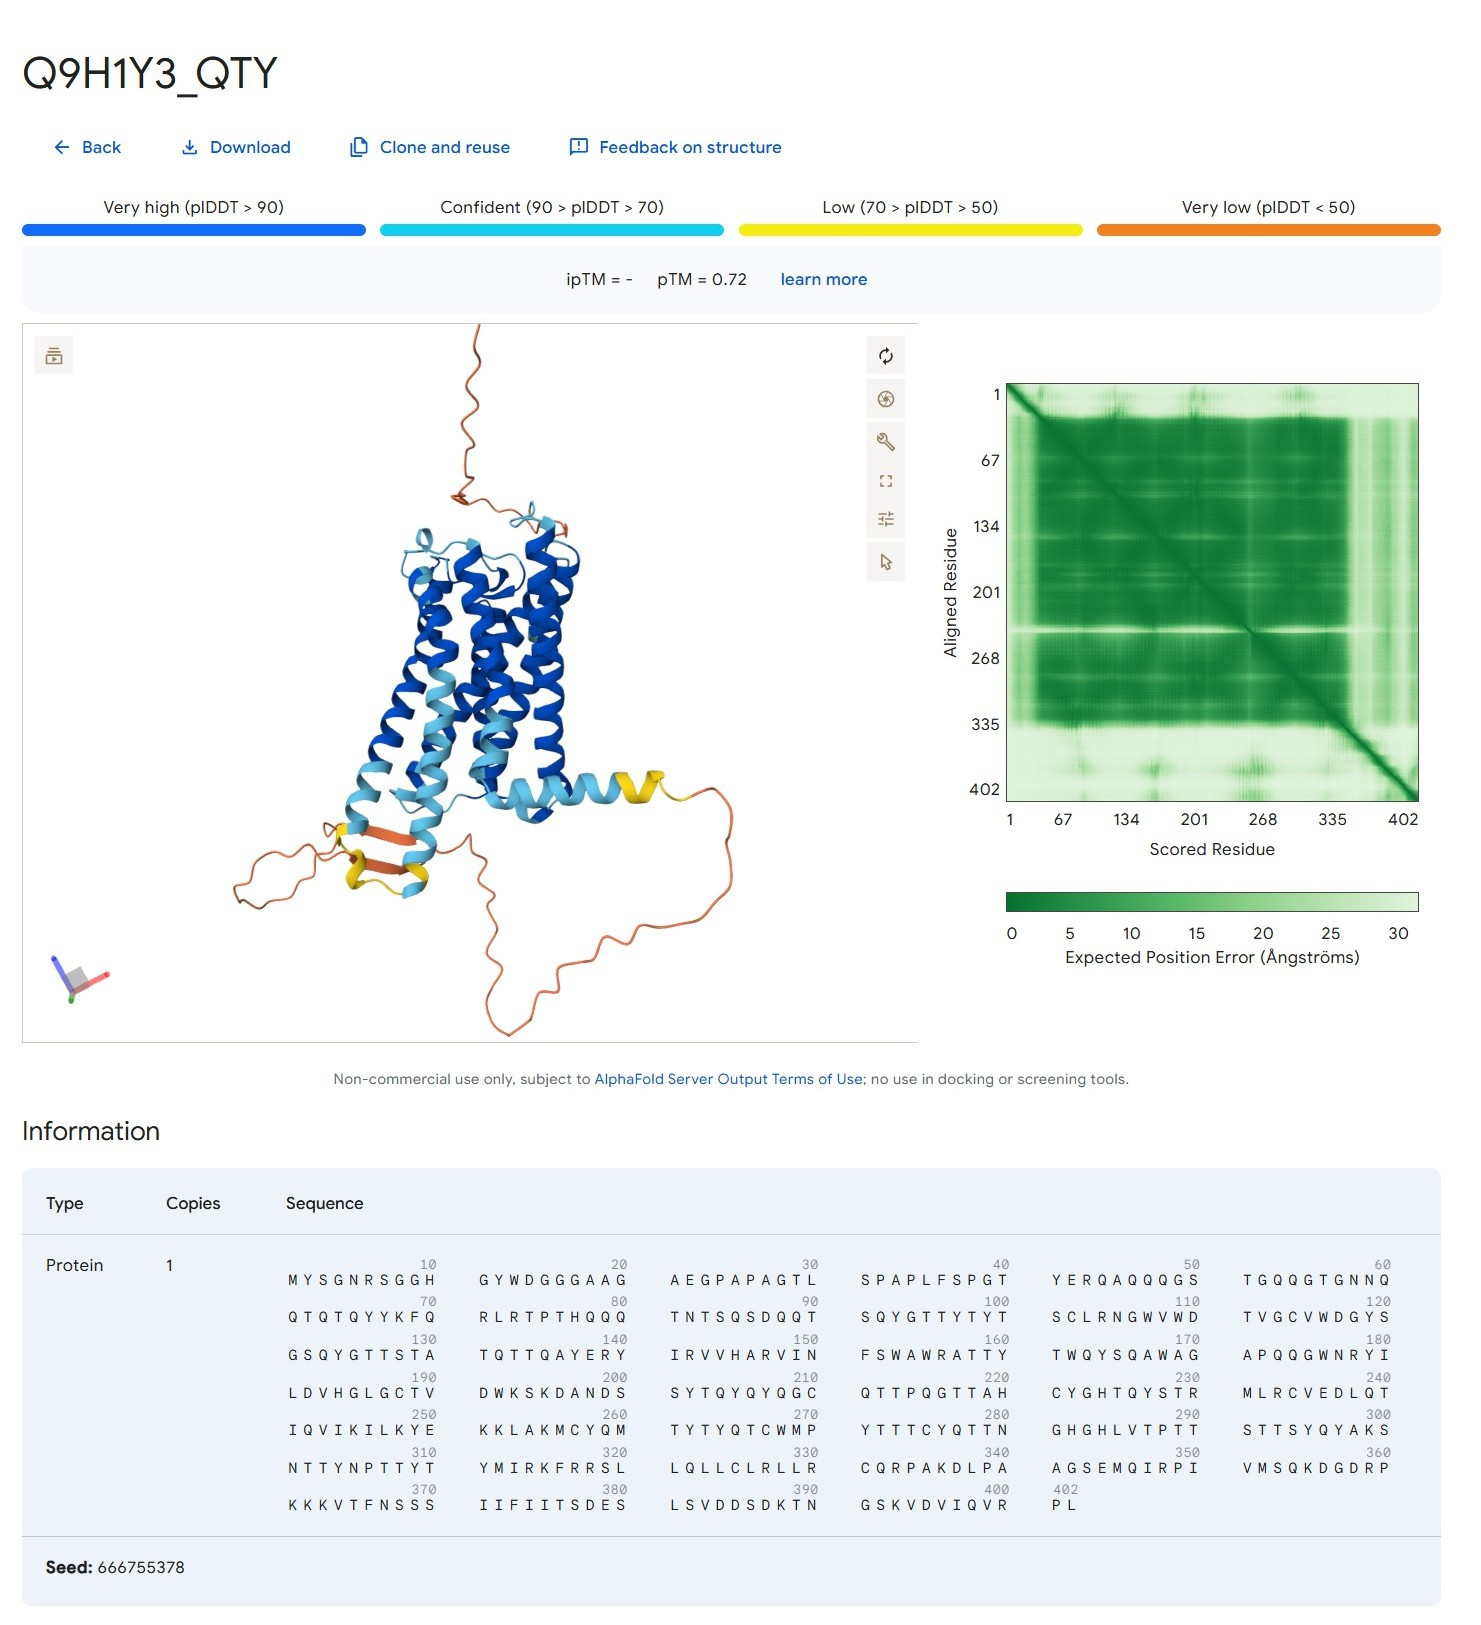
\includegraphics[width=\linewidth]{SuppFigures/af3 opn3 qty.jpg}
\end{figure}

\newpage
\begin{figure}[H]
    \textbf{f)} OPN4$^{\textrm{QTY}}$ \\
    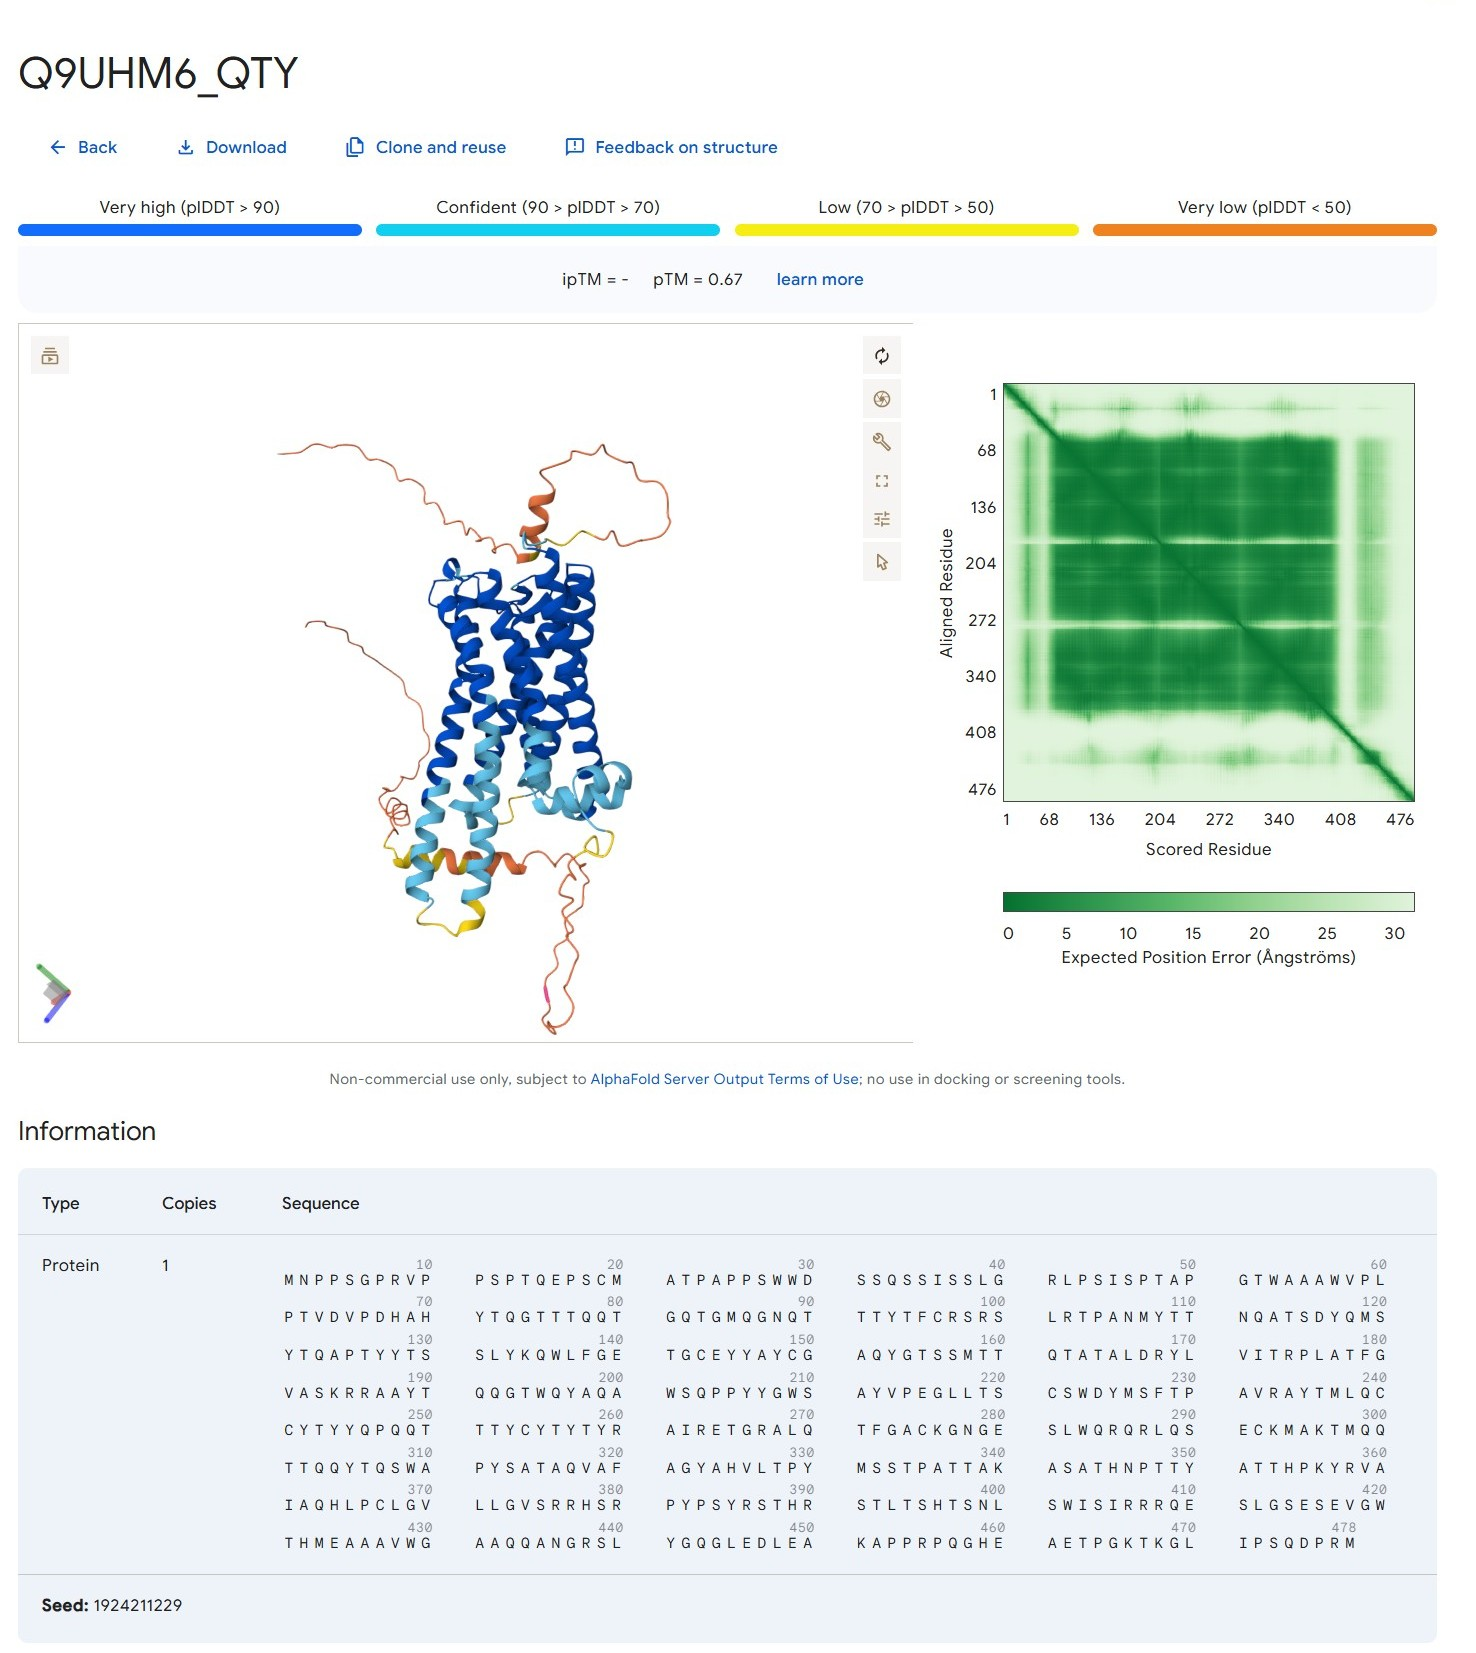
\includegraphics[width=\linewidth]{SuppFigures/af3 opn4 qty.jpg}
\end{figure}

\newpage
\begin{figure}[H]
    \textbf{g)} OPN5$^{\textrm{QTY}}$ \\
    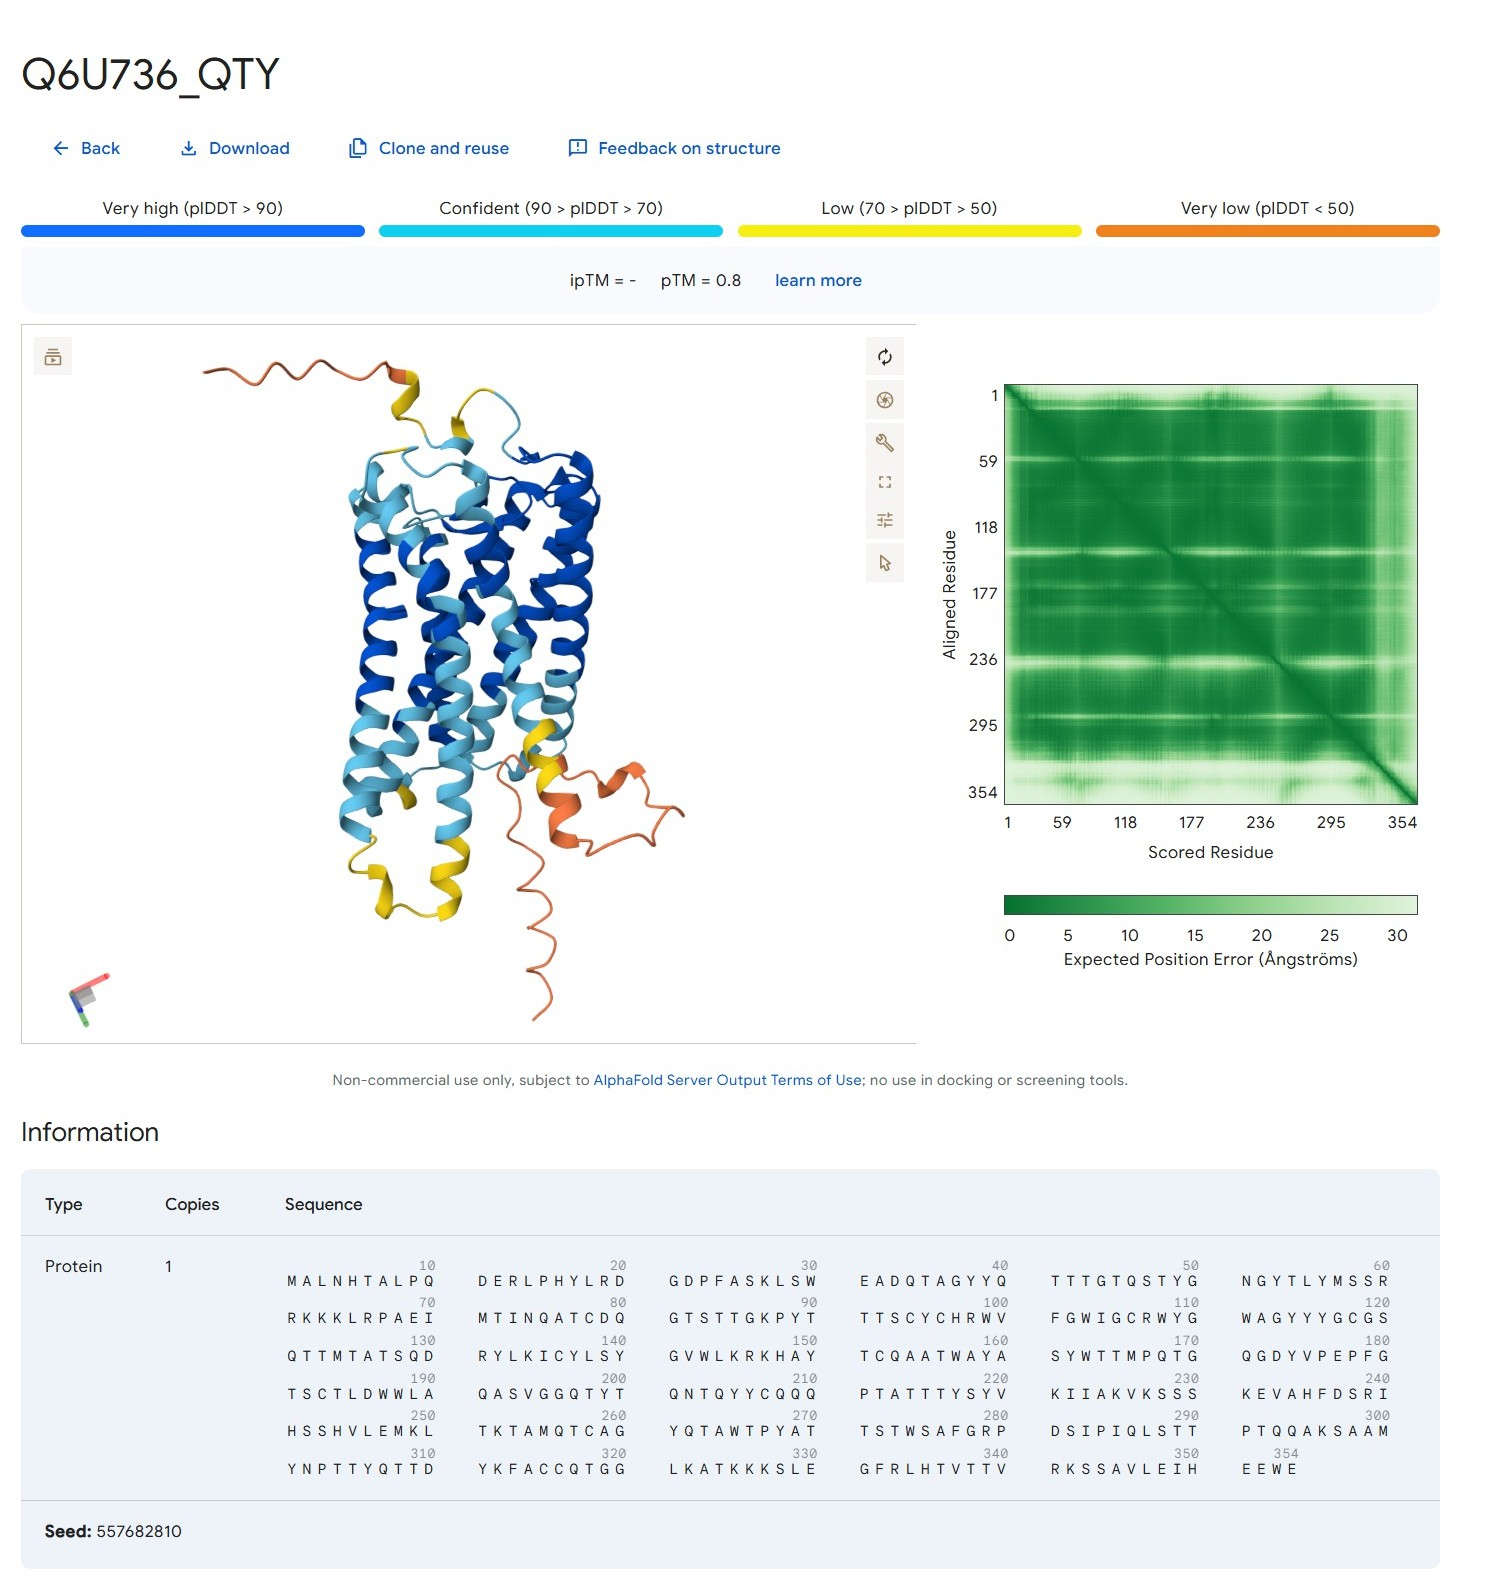
\includegraphics[width=\linewidth]{SuppFigures/af3 opn5 qty.jpg}
\end{figure}

\newpage
\begin{figure}[H]
    \textbf{h)} RGR$^{\textrm{QTY}}$ \\
    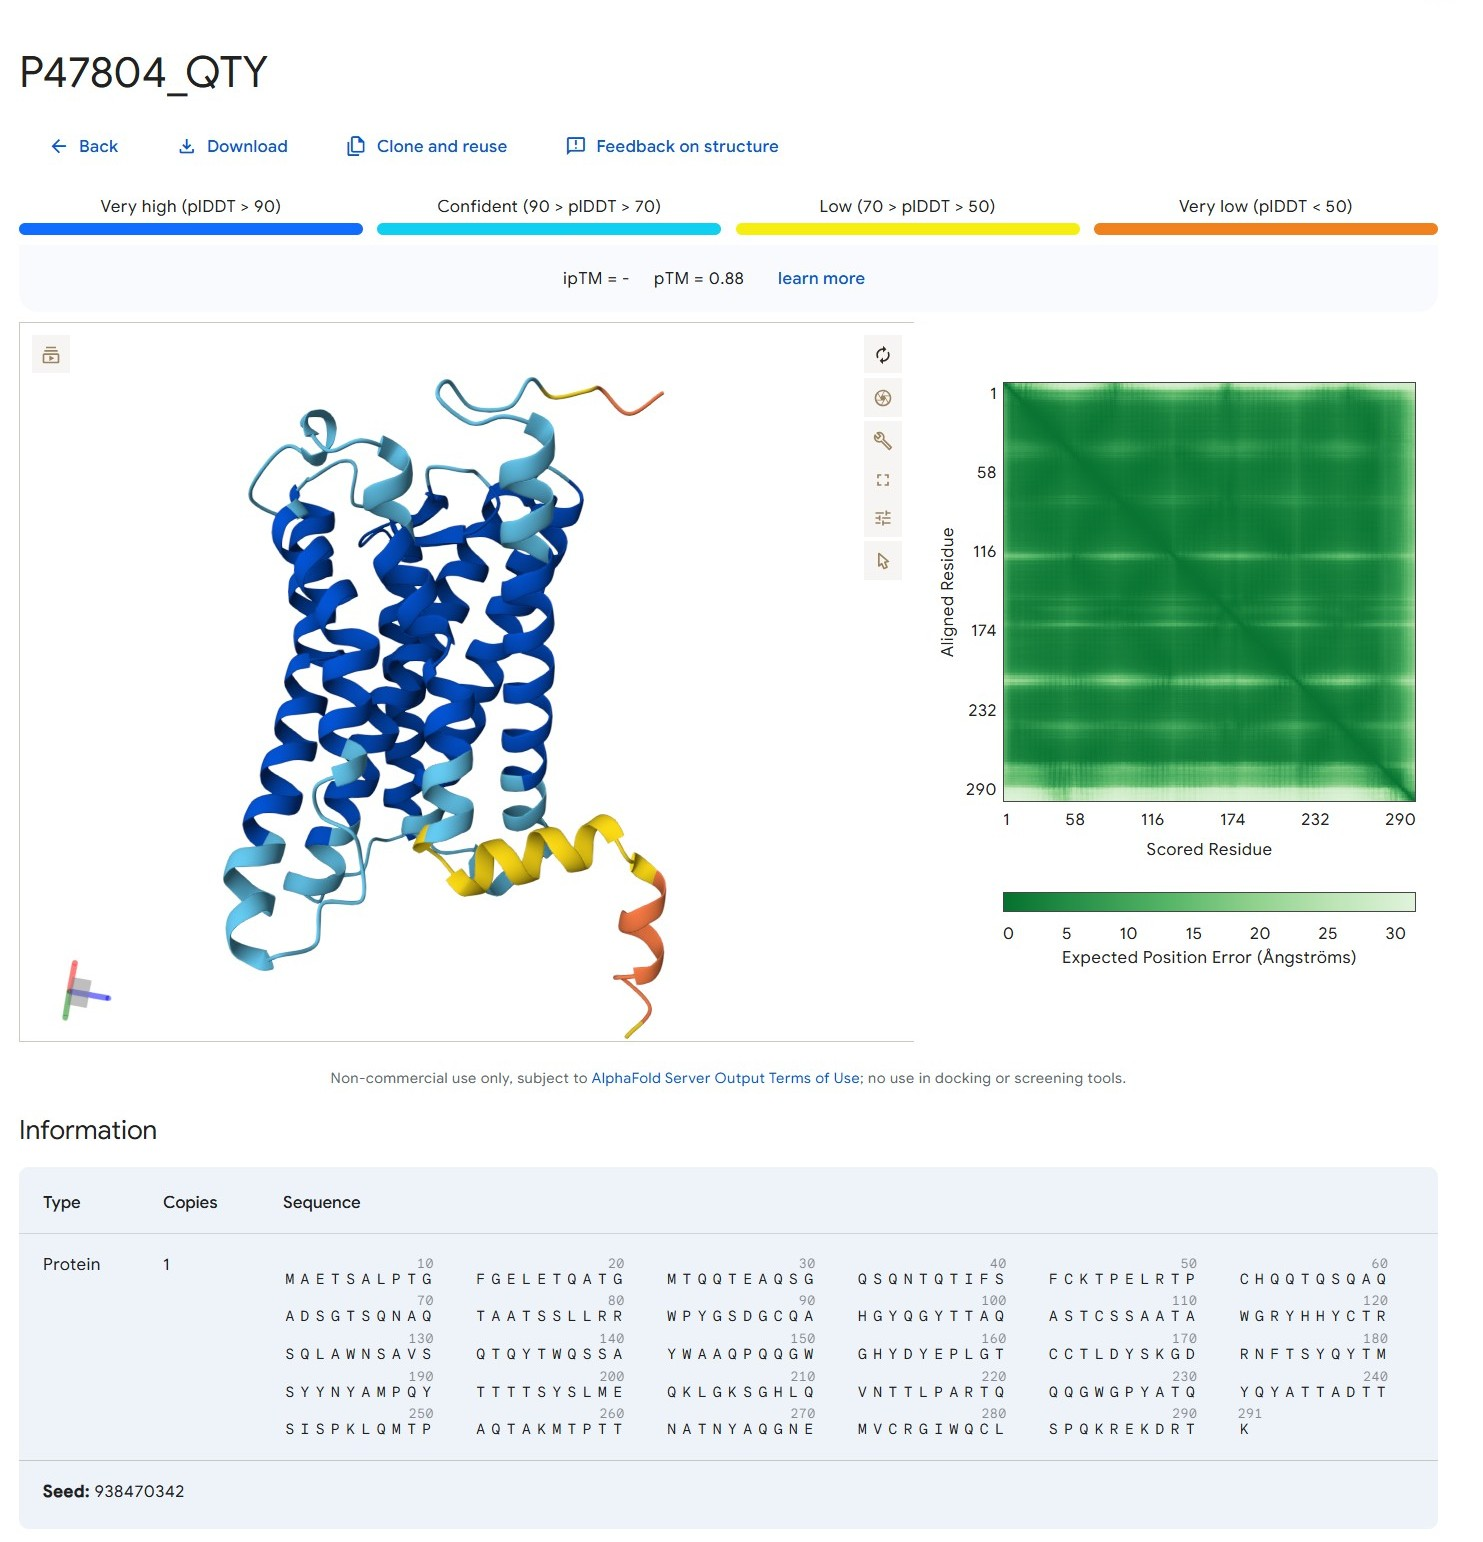
\includegraphics[width=\linewidth]{SuppFigures/af3 rgr qty.jpg}
\end{figure}

\newpage
\begin{figure}[H]
    \textbf{i)} RRH$^{\textrm{QTY}}$ \\
    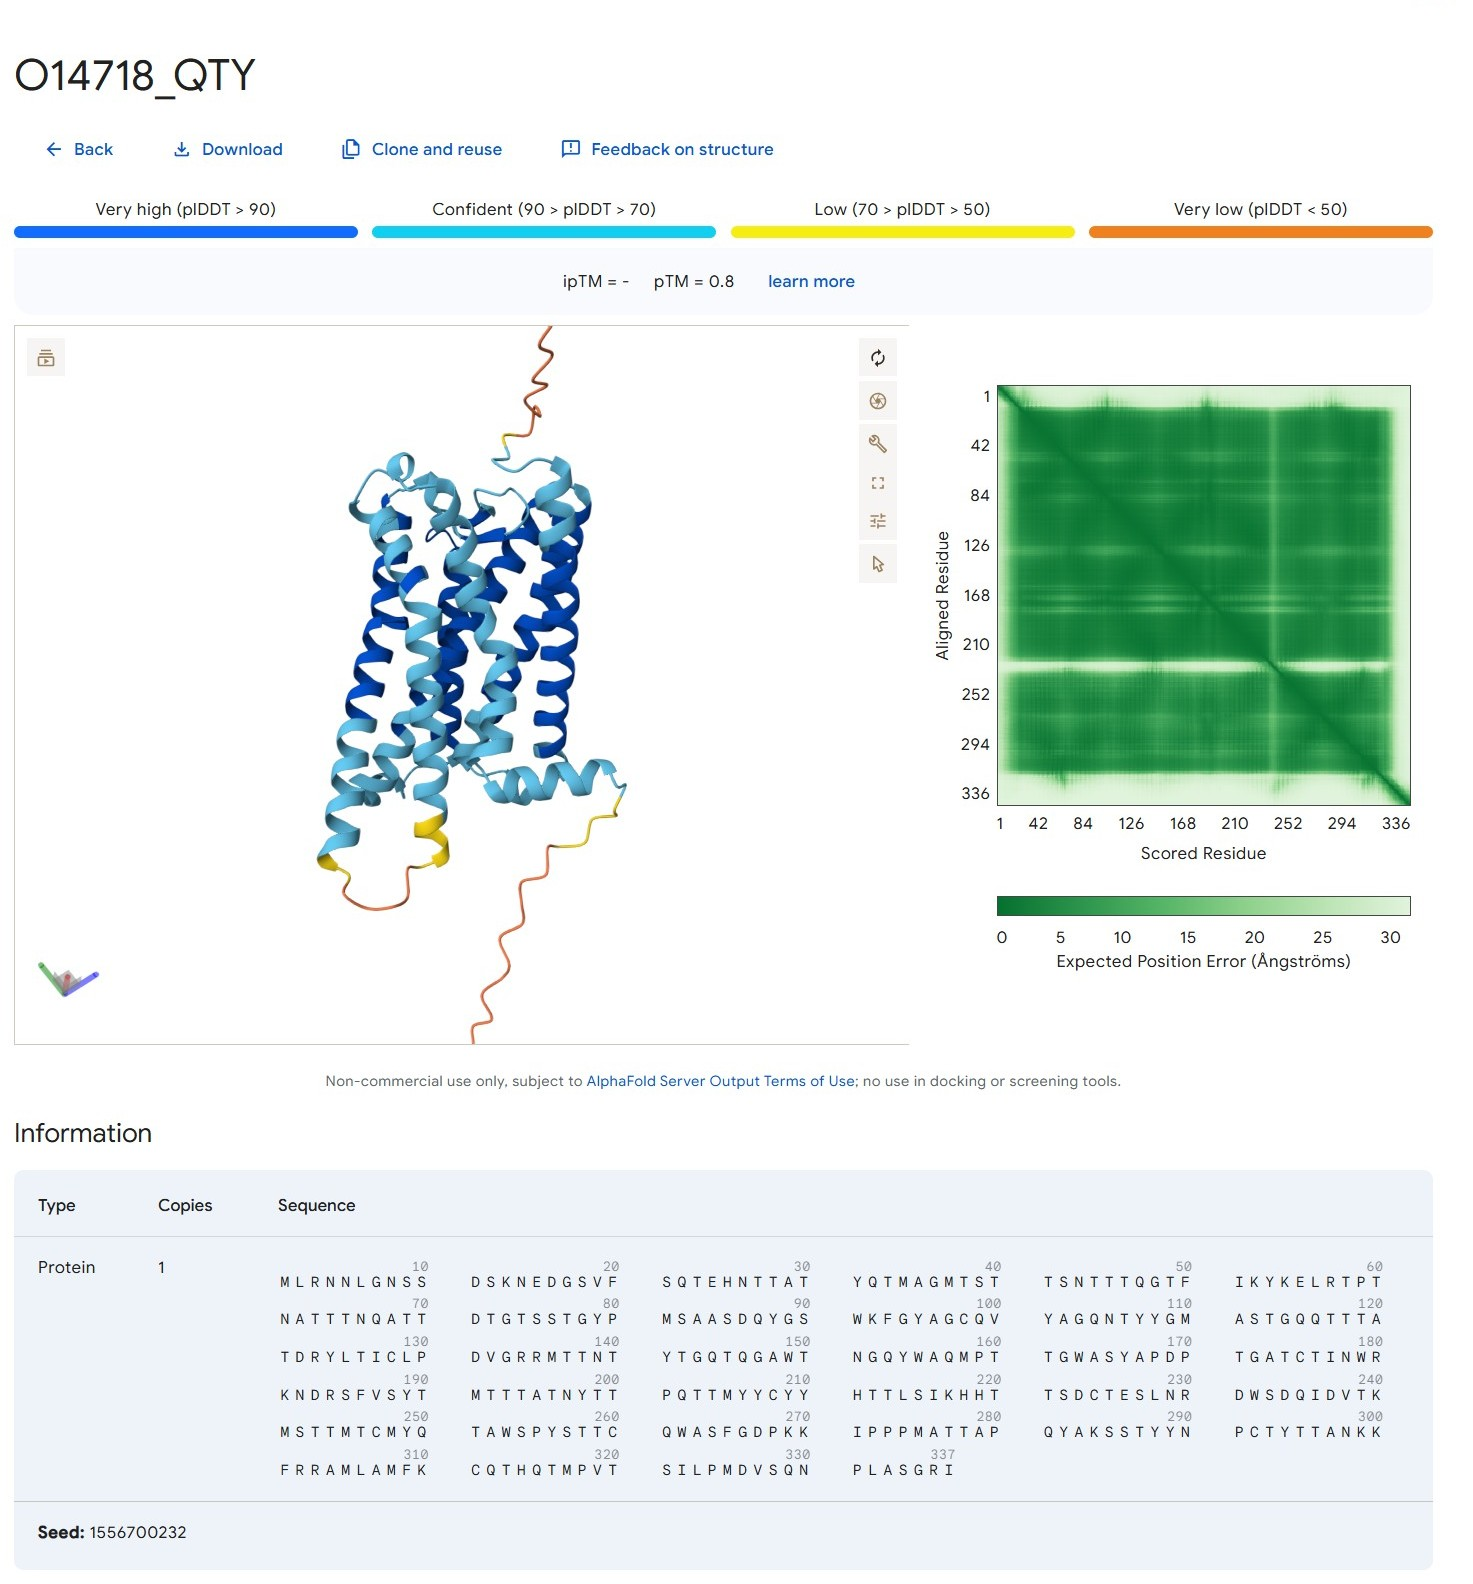
\includegraphics[width=\linewidth]{SuppFigures/af3 rrh qty.jpg}
\end{figure}

\newpage
\begin{figure}[H]
    \textbf{j)} BACR$^{\textrm{QTY}}$ \\
    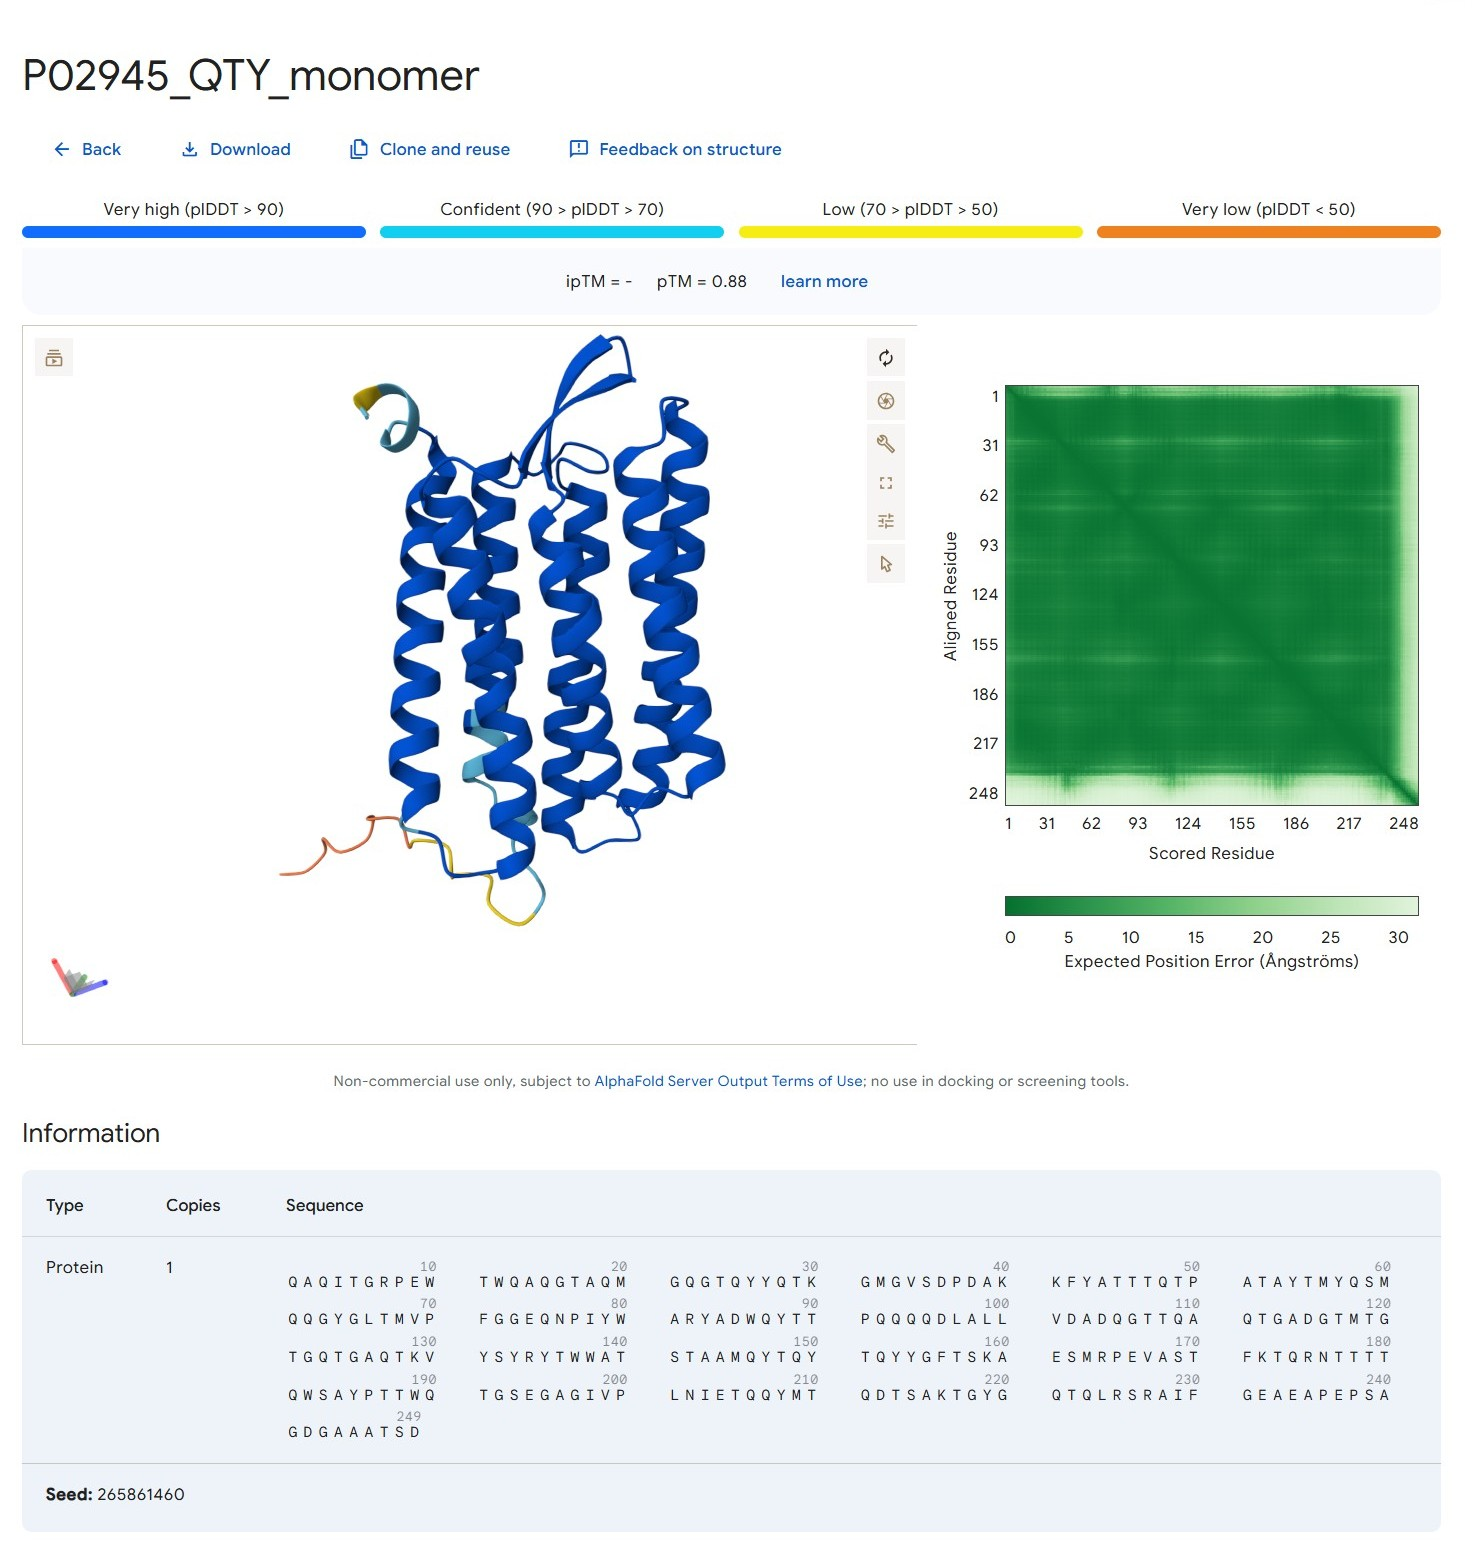
\includegraphics[width=\linewidth]{SuppFigures/af3 bacr qty mono.jpg}
\end{figure}

\newpage
\begin{figure}[H]
    \textbf{k)} BACH$^{\textrm{QTY}}$ \\
    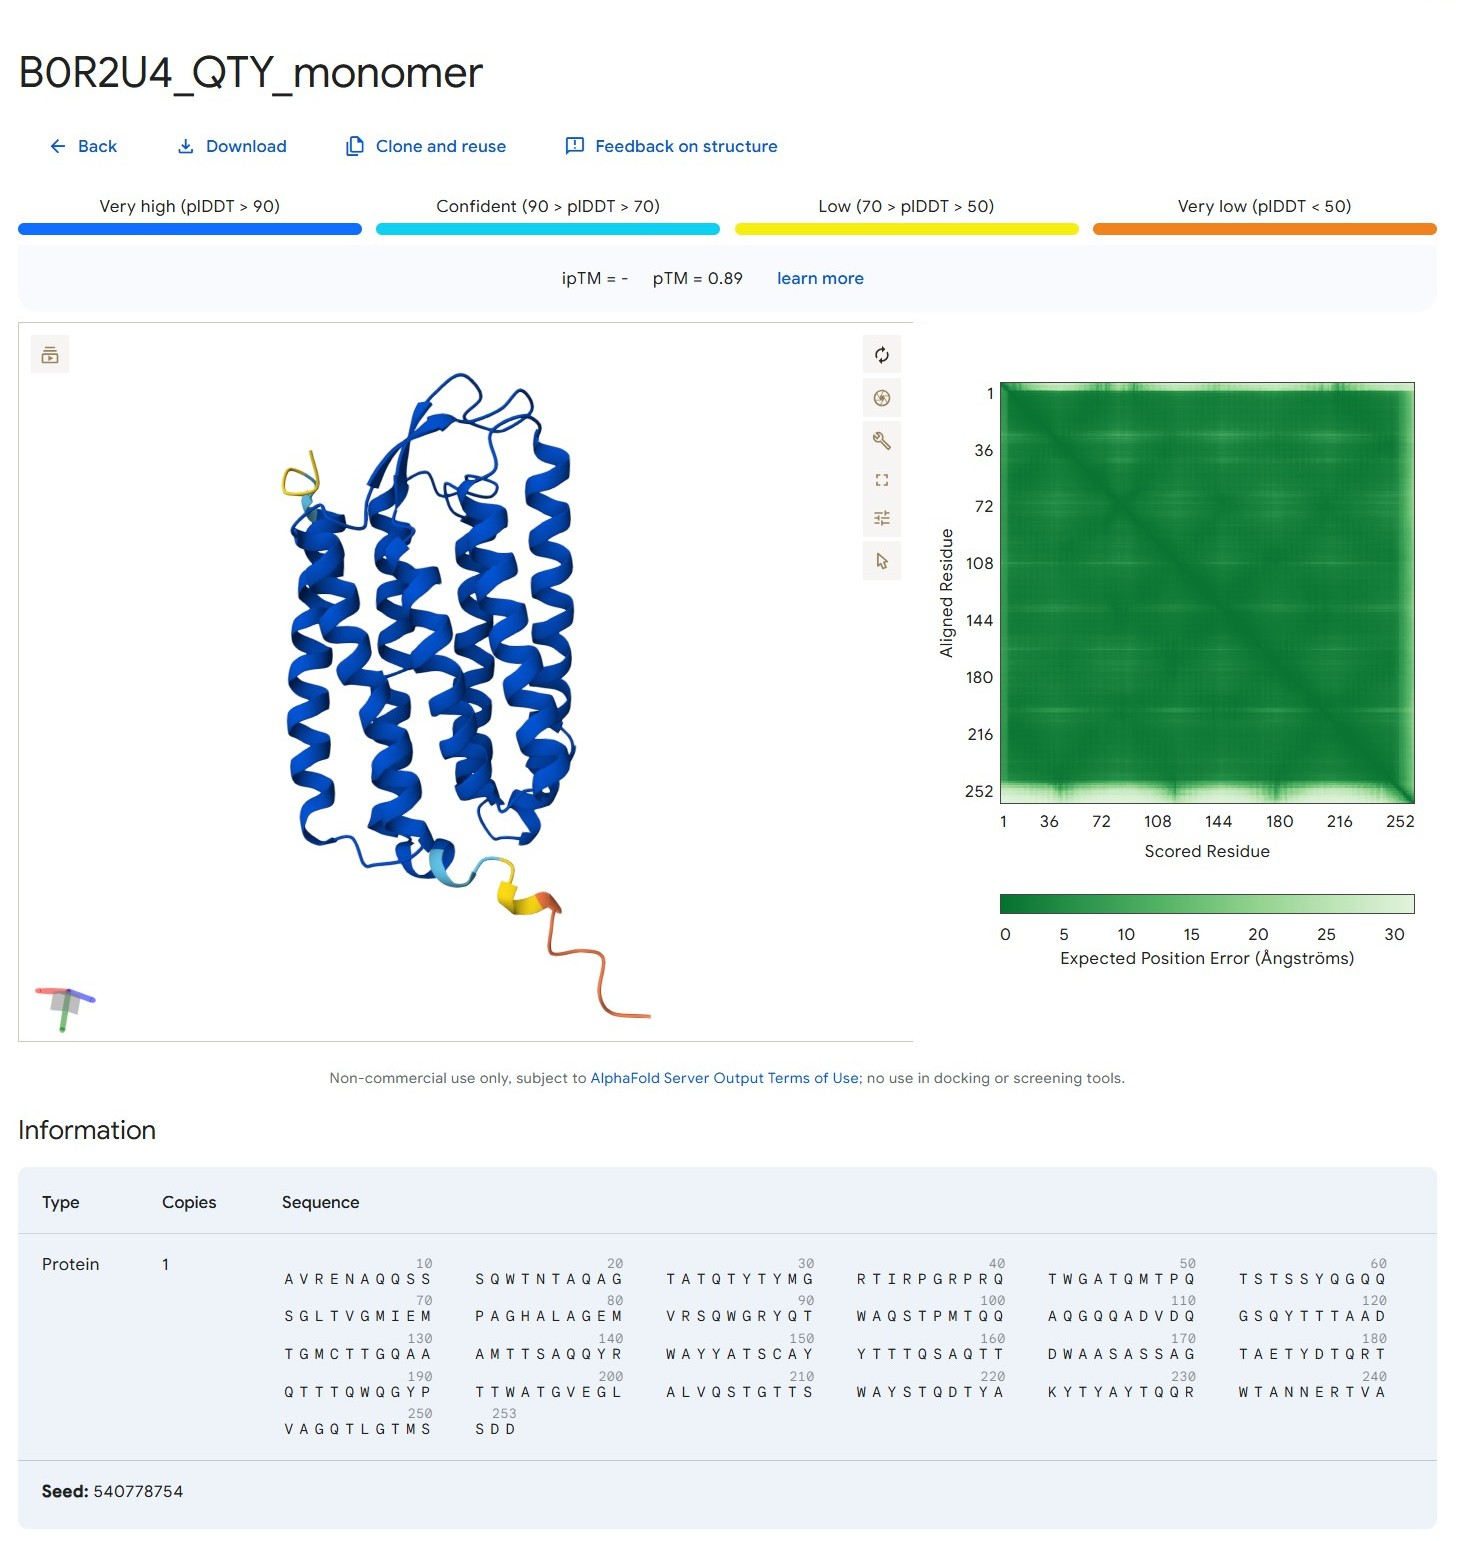
\includegraphics[width=\linewidth]{SuppFigures/af3 bach qty mono.jpg}
\end{figure}

\newpage
\begin{figure}[H]
    \textbf{l)} ChR2$^{\textrm{QTY}}$ \\
    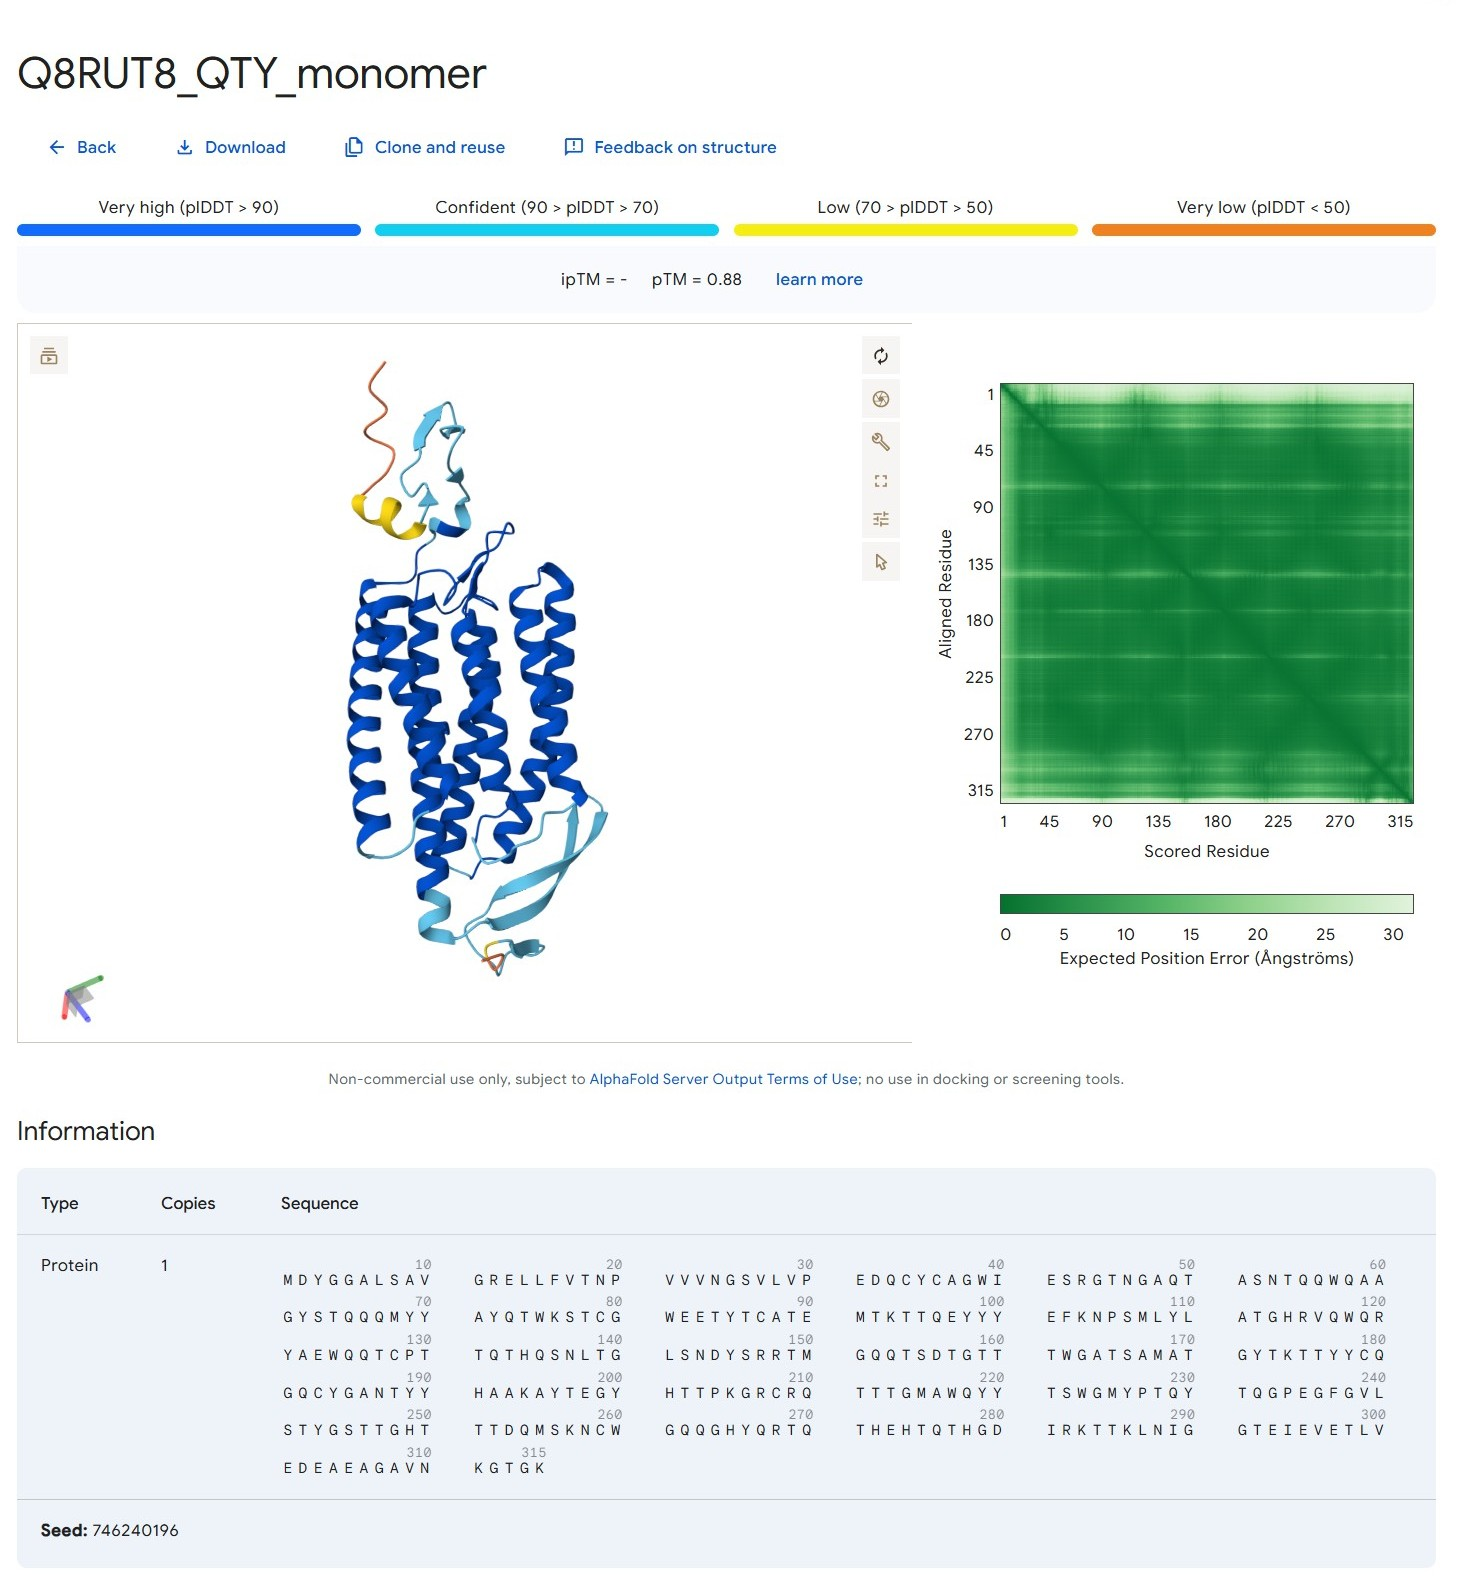
\includegraphics[width=\linewidth]{SuppFigures/af3 chr2 qty mono.jpg}
\end{figure}

\newpage
\begin{figure}[H]
    \textbf{m)} BACR$^{\textrm{QTY}}$ \\
    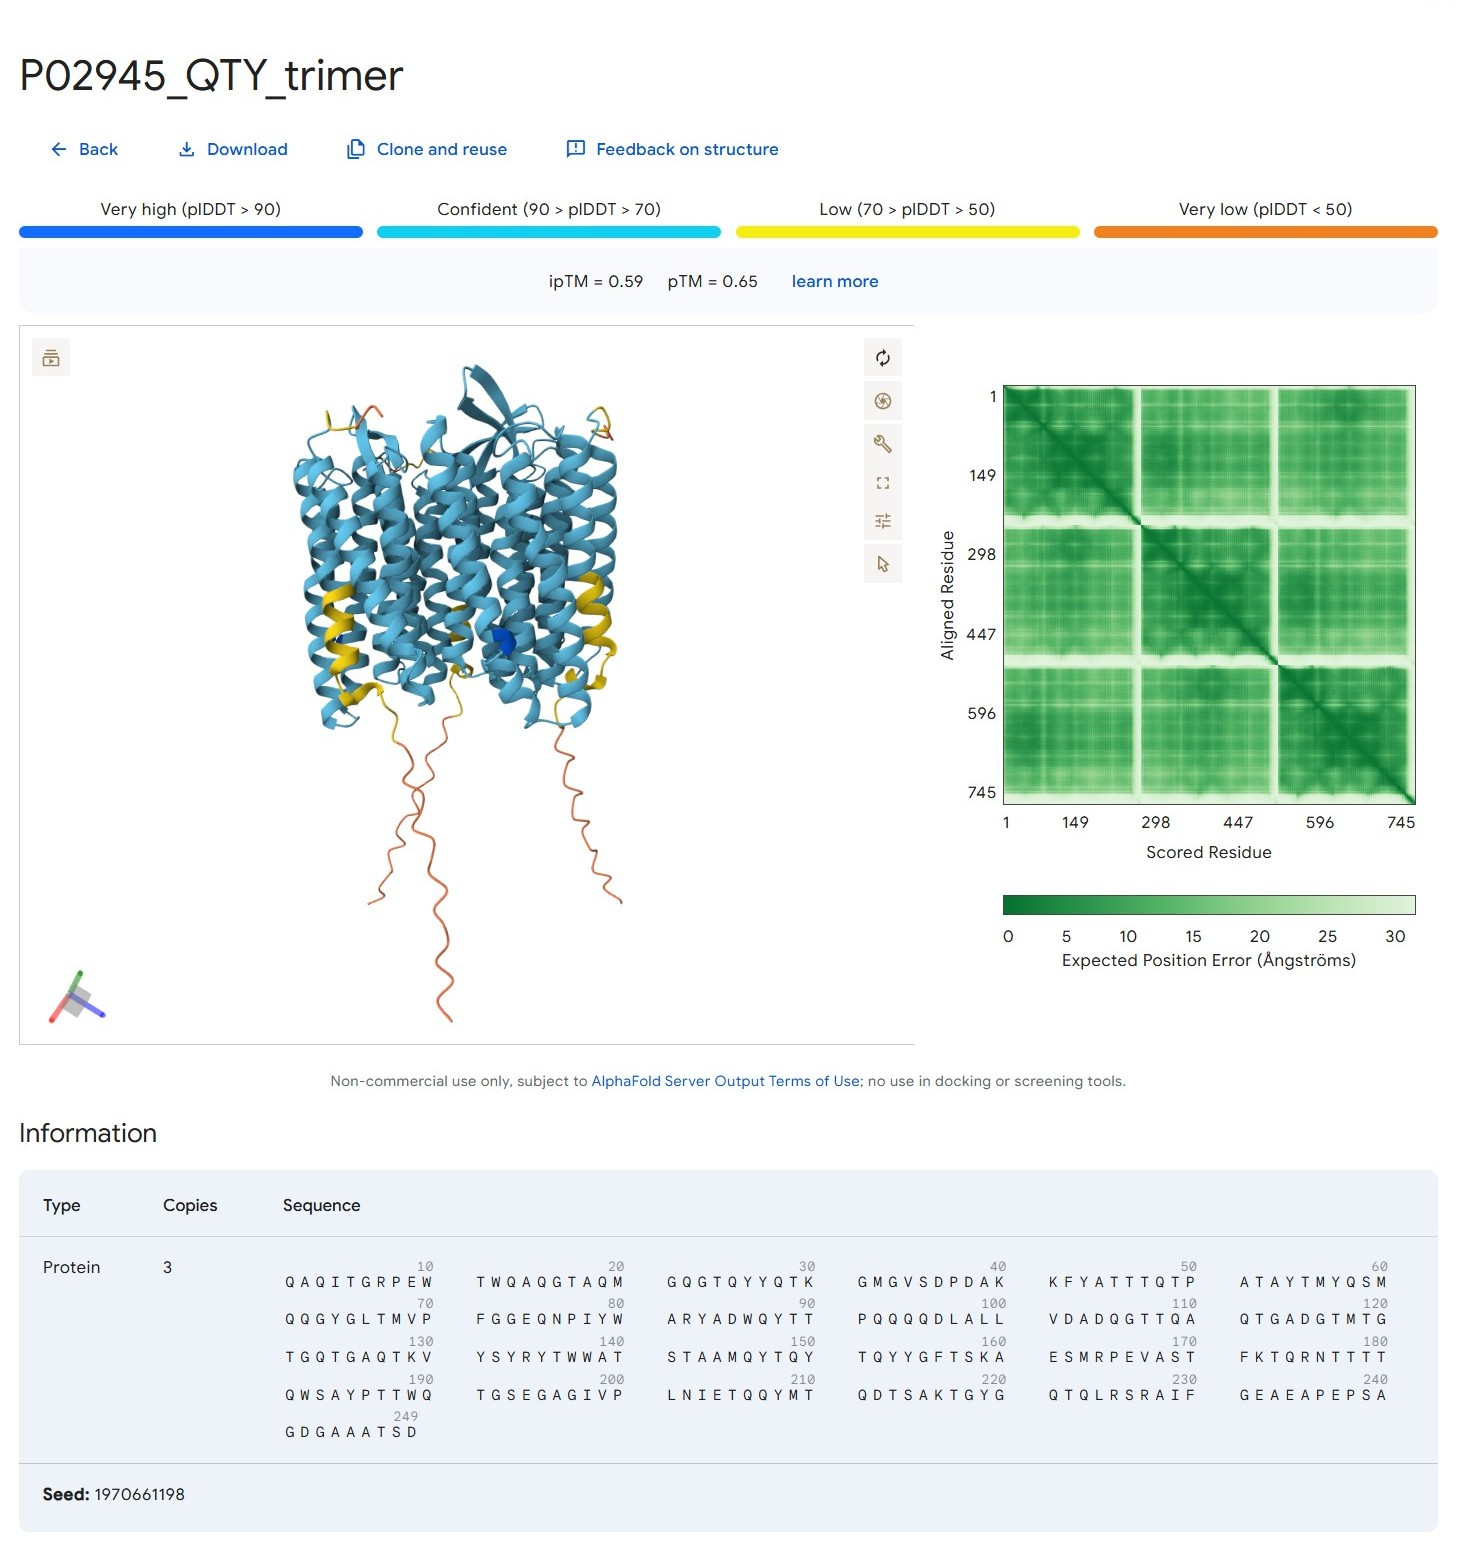
\includegraphics[width=\linewidth]{SuppFigures/af3 bacr qty tri.jpg}
\end{figure}

\newpage
\begin{figure}[H]
    \textbf{n)} BACH$^{\textrm{QTY}}$ \\
    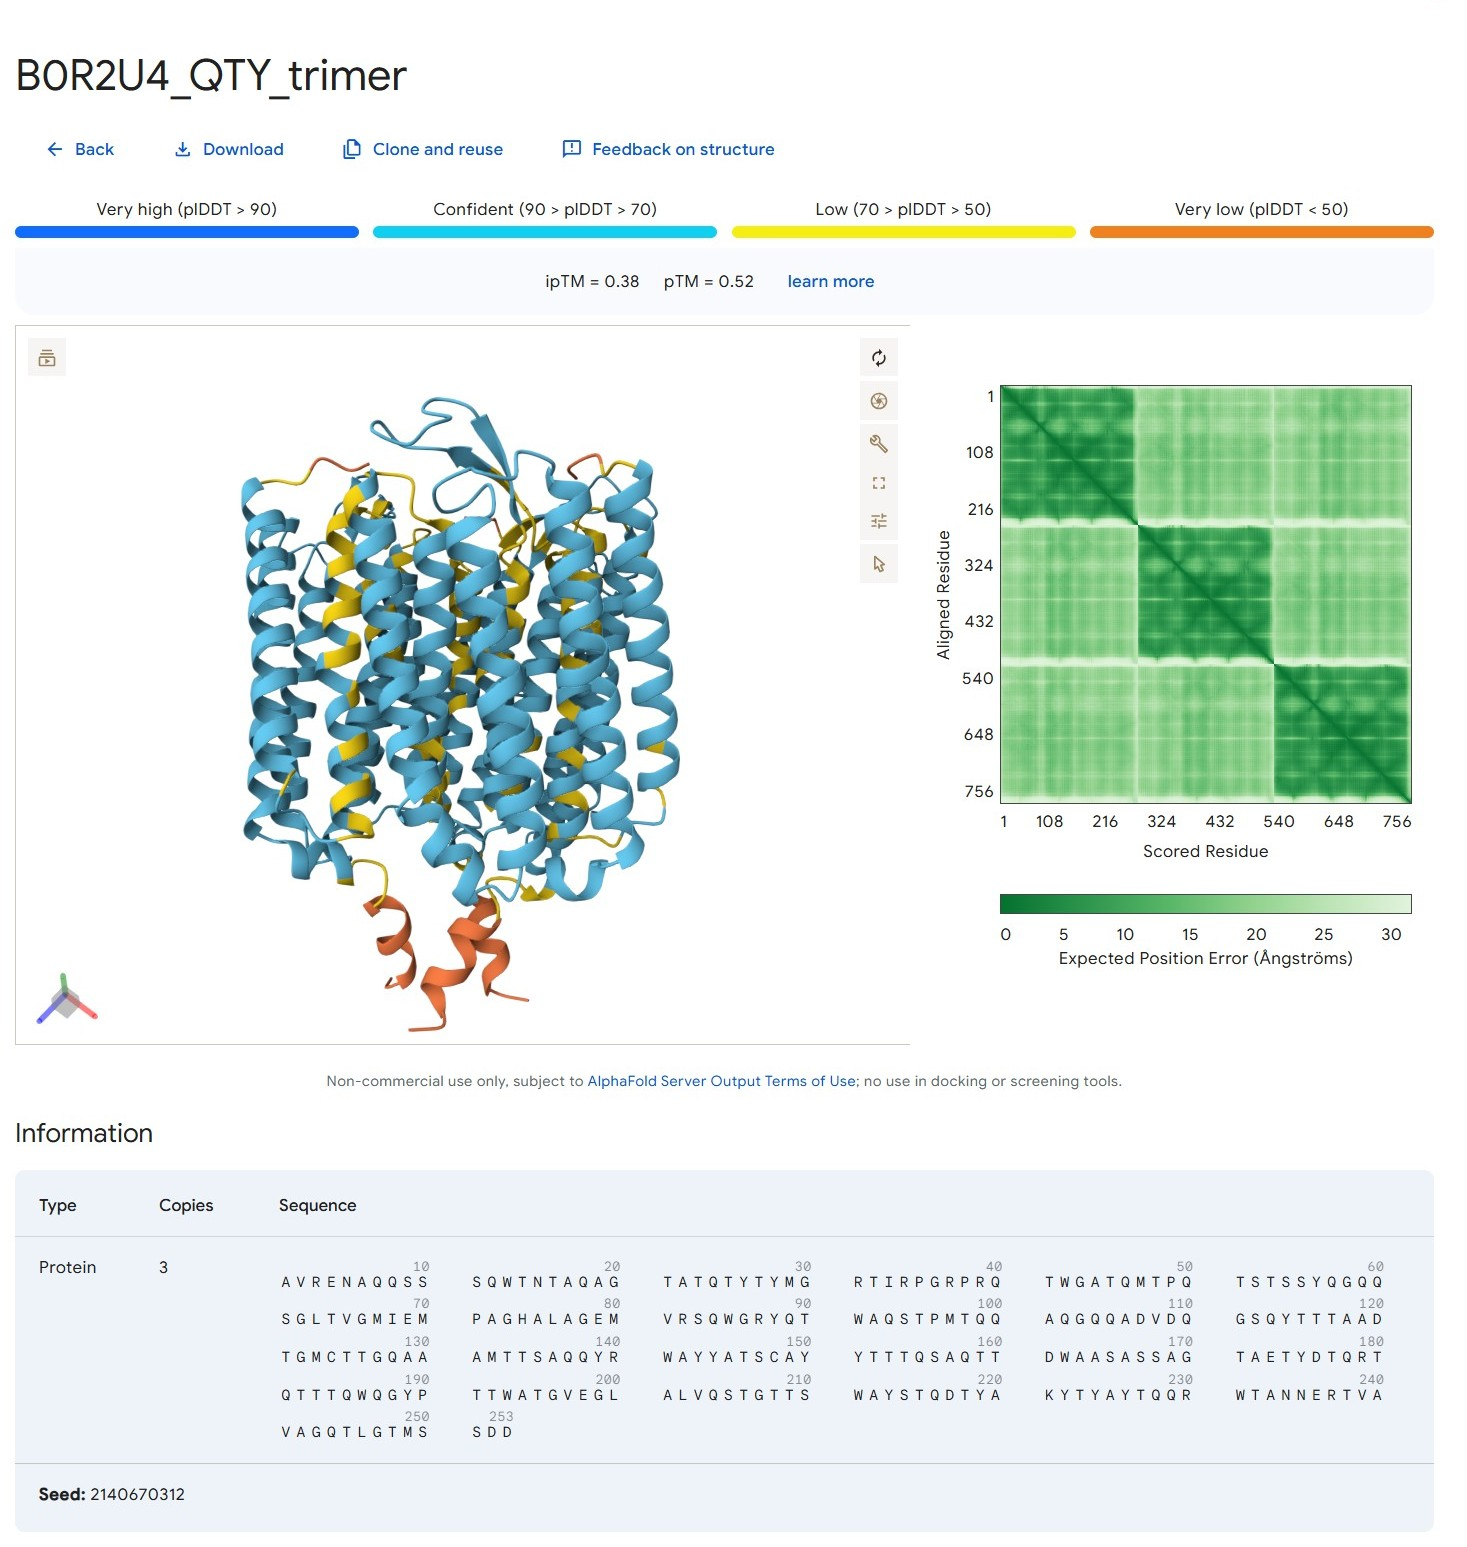
\includegraphics[width=\linewidth]{SuppFigures/af3 bach qty tri.jpg}
\end{figure}

\newpage
\begin{figure}[H]
    \textbf{o)} ChR2$^{\textrm{QTY}}$ \\
    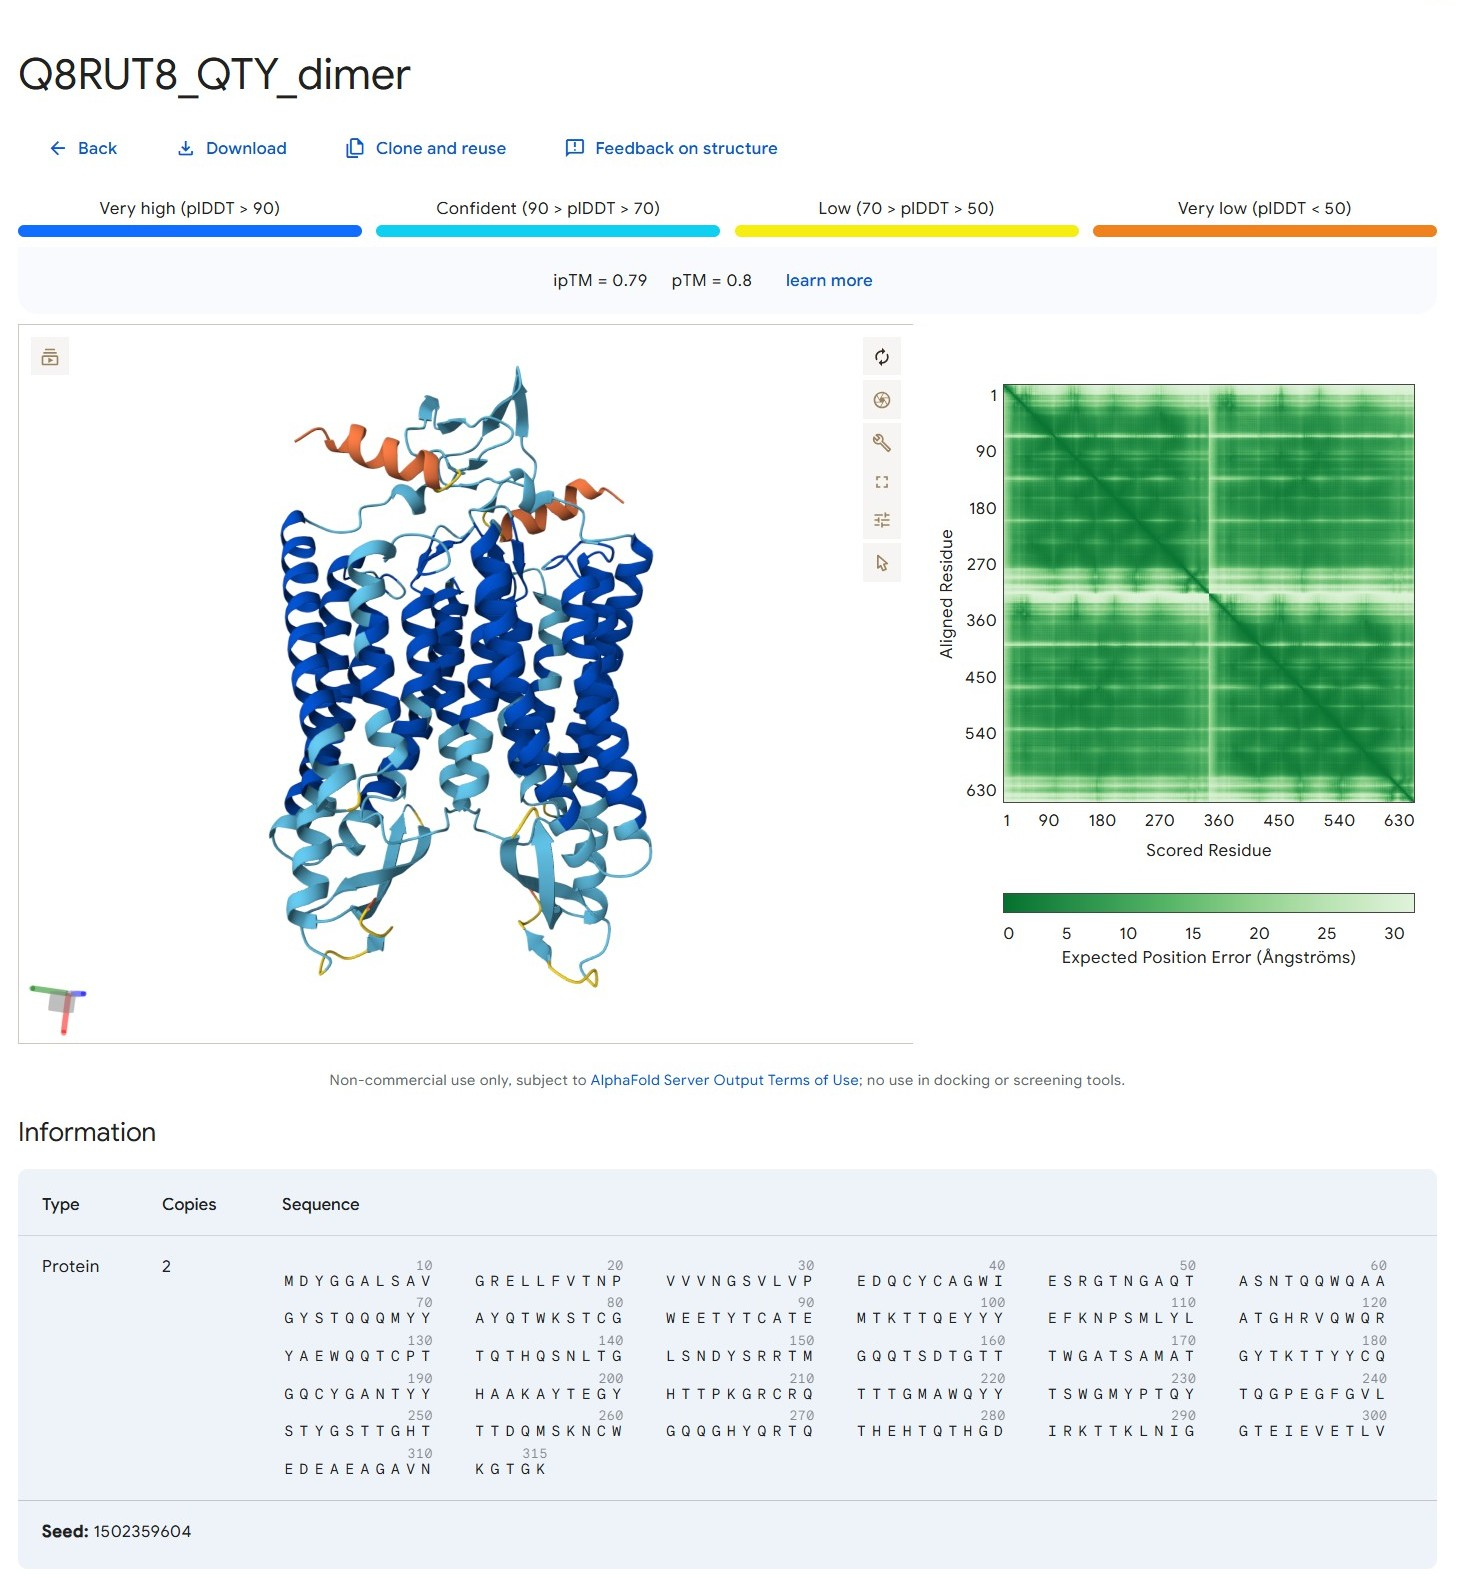
\includegraphics[width=\linewidth]{SuppFigures/af3 chr2 qty di.jpg}
\end{figure}

\begin{figure}[H]
    \caption{\textbf{The radius of gyration of native and QTY-designed OPN2. } By convention, the isomerization is set at time 0ns, which is indicated by a brown, vertical dashed line. The radius of gyration and its 1-ns running average are shown, respectively, as black and red lines. }
    \textbf{a)} Native OPN2 \\ \\
    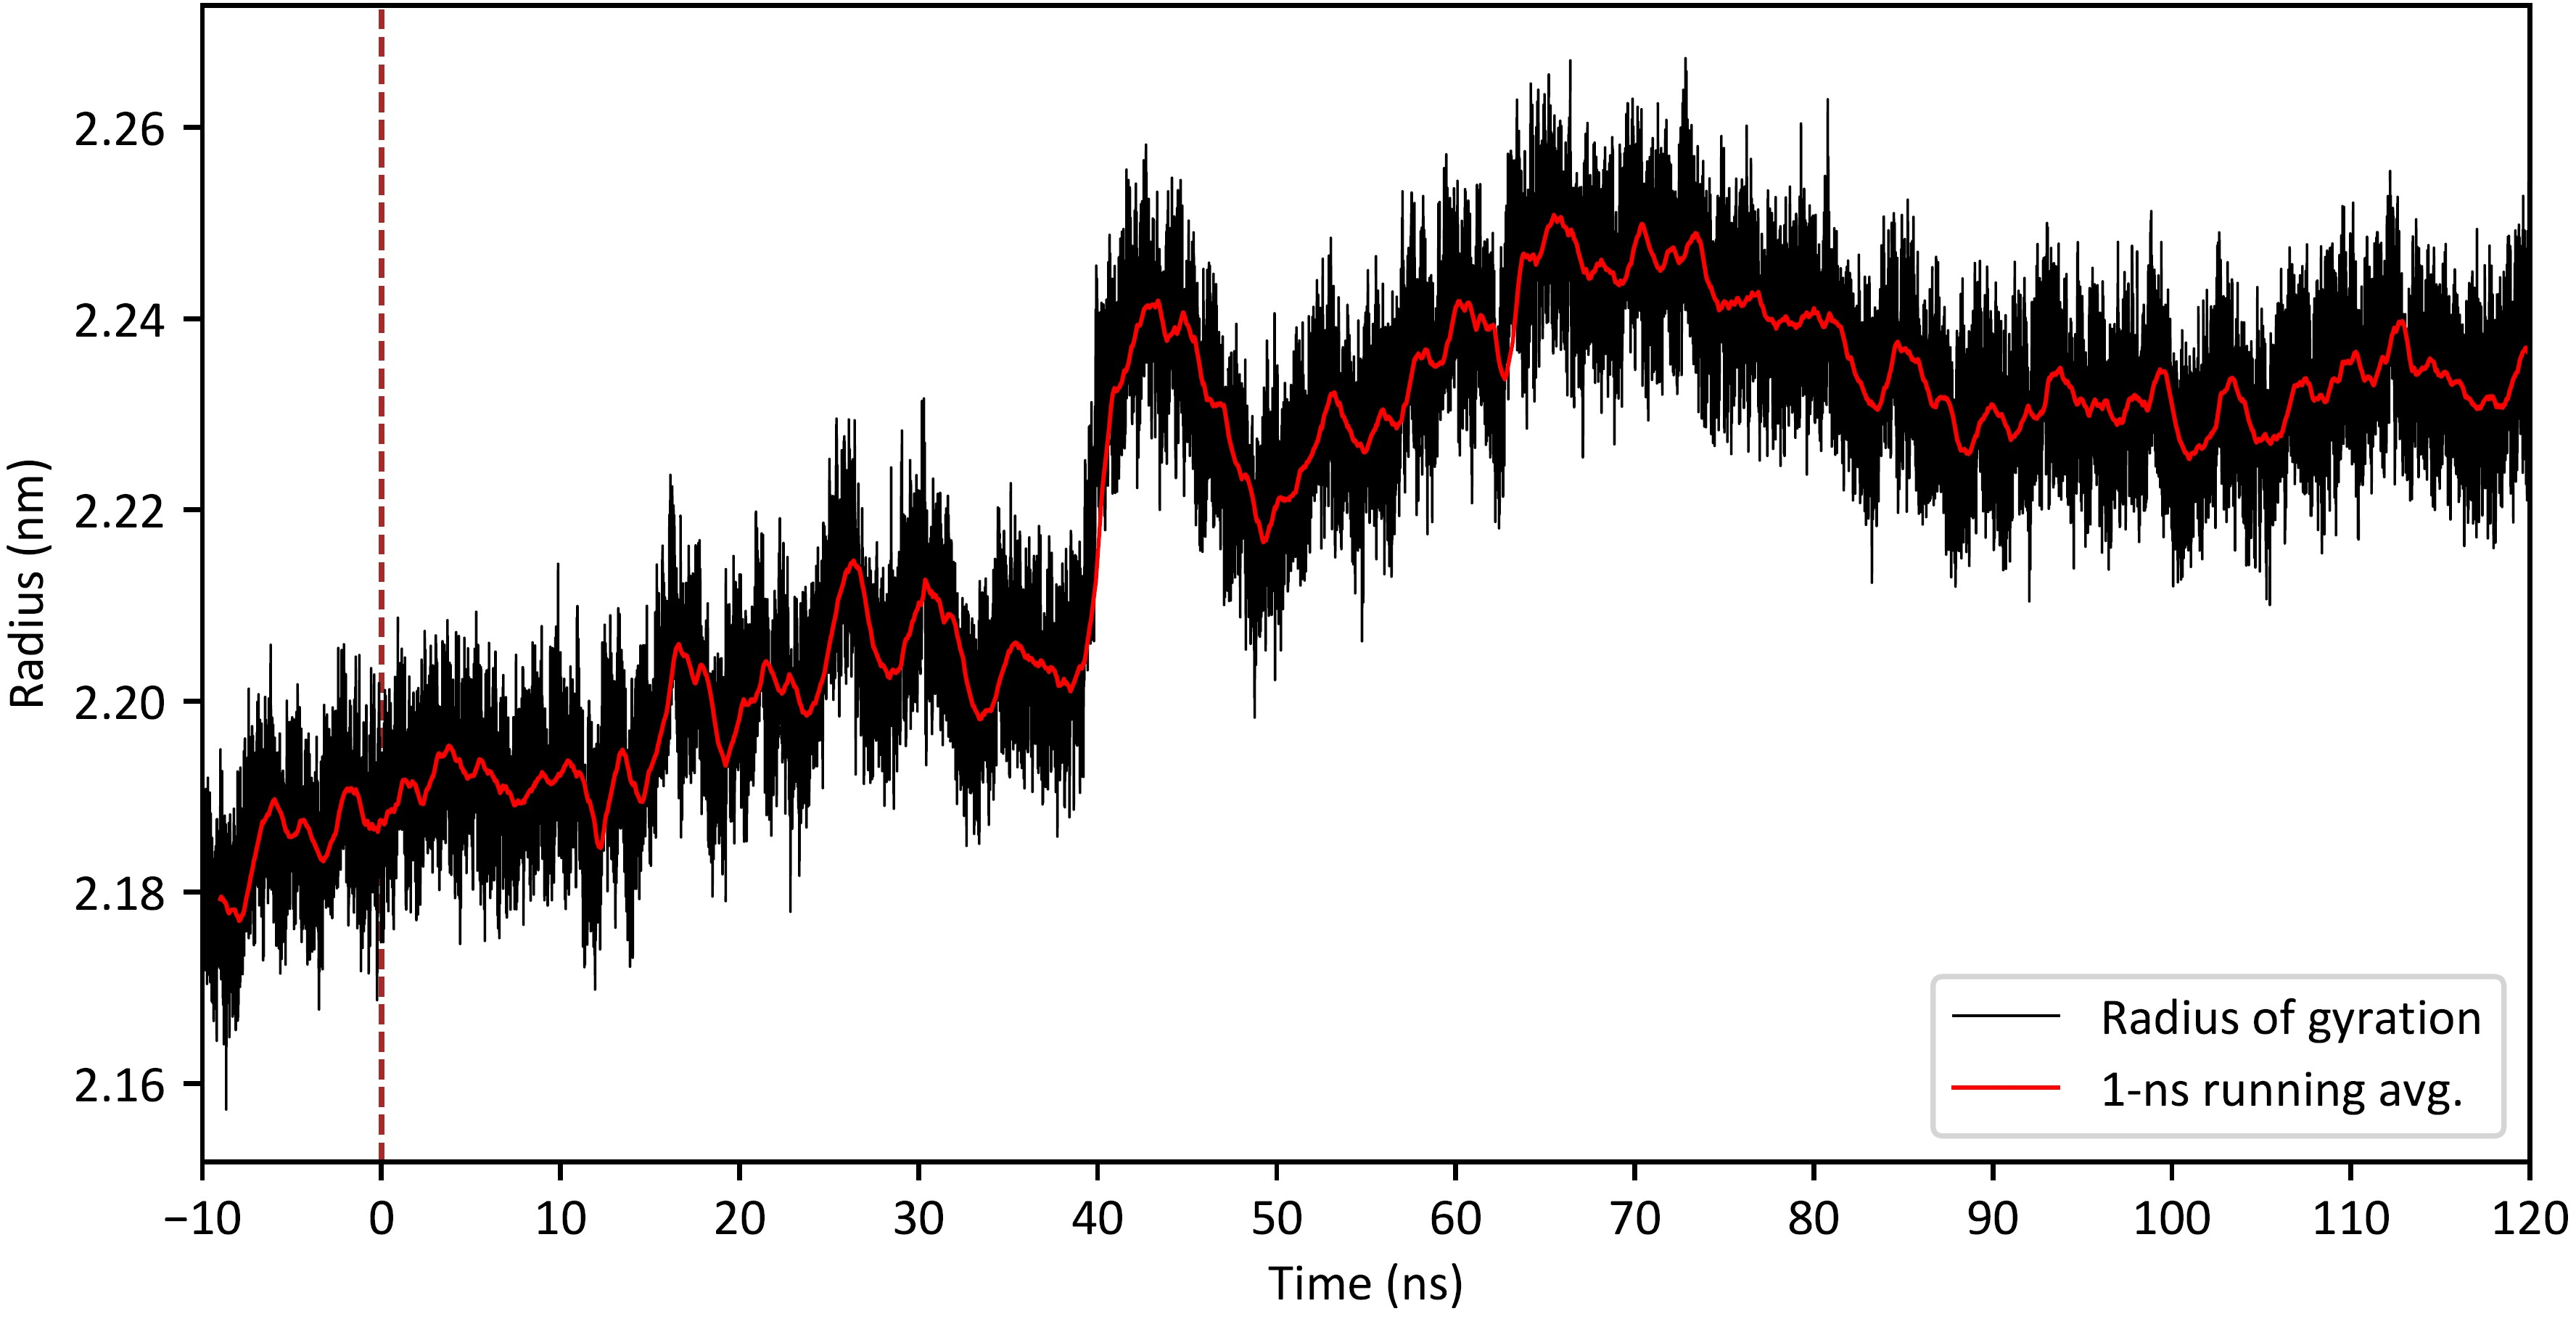
\includegraphics[width=\linewidth]{SuppFigures/wt gyrate.jpg}
    \textbf{b)} QTY-designed OPN2 \\ \\
    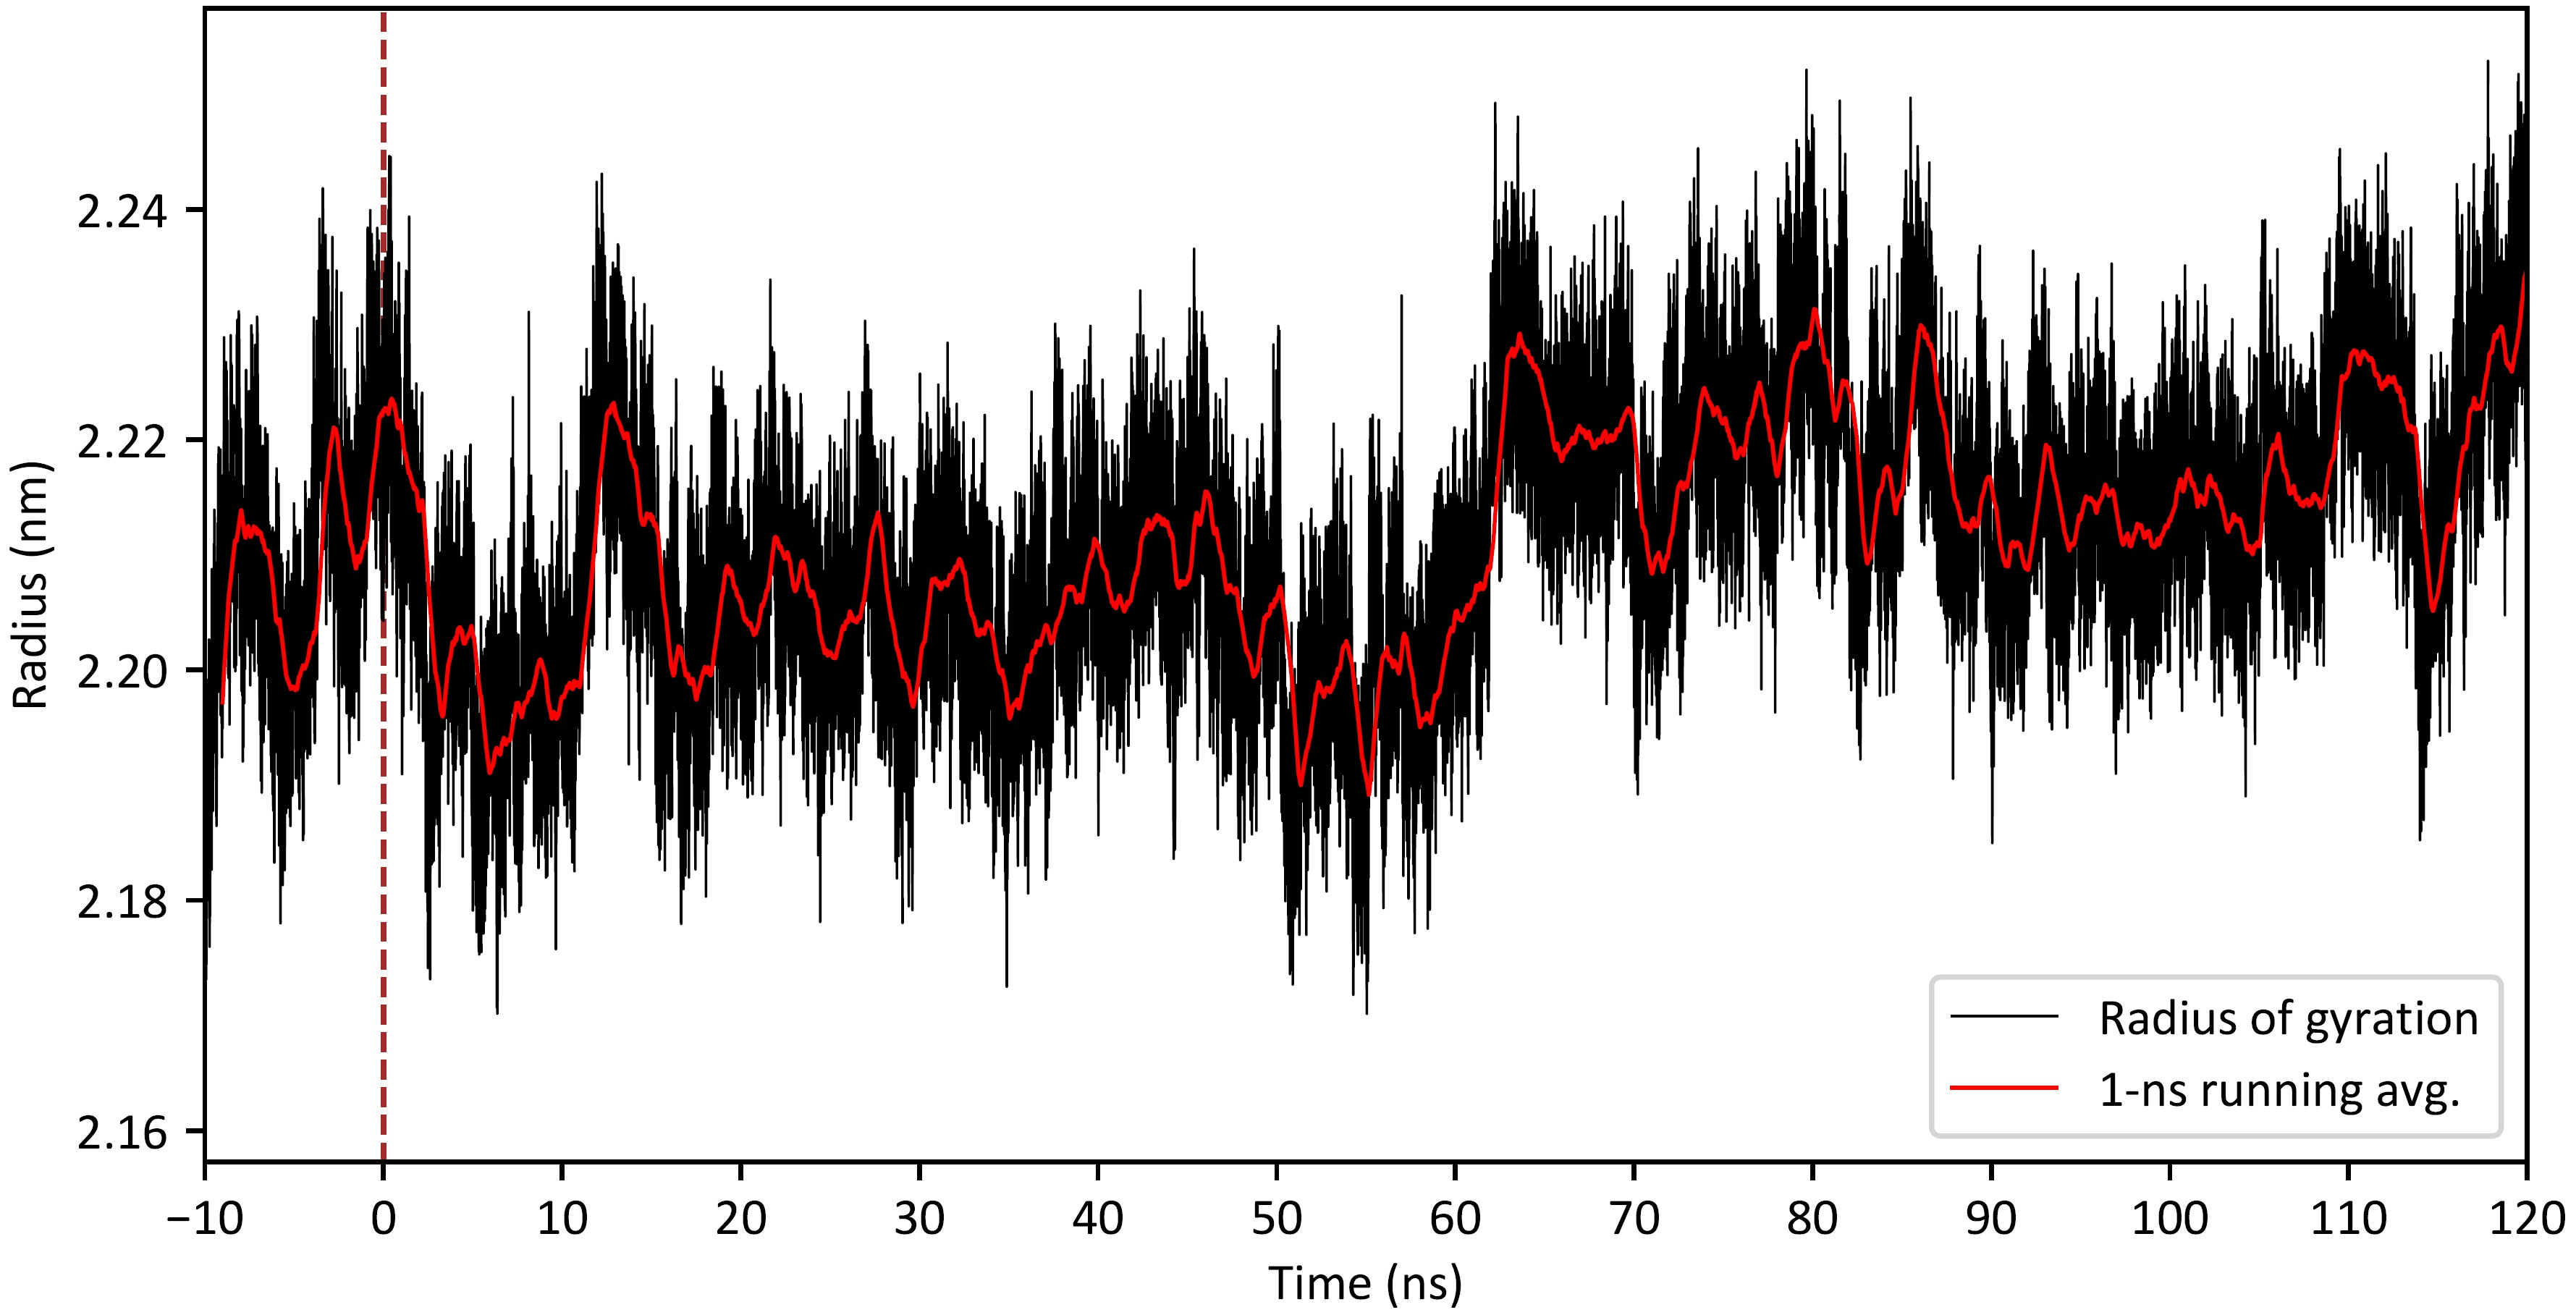
\includegraphics[width=\linewidth]{SuppFigures/qty gyrate.jpg}
\end{figure}

\begin{figure}[H]
    \caption{\textbf{The root mean square (RMS) fluctuation of native and QTY-designed OPN2. } Blue bars represent proteins with 11-cis-retinal and yellow bars represent proteins with all-trans-retinal. The two states are plotted on the same set of axis, with the shorter bars placed on top of the taller bars. }
    \textbf{a)} Native OPN2 \\ \\
    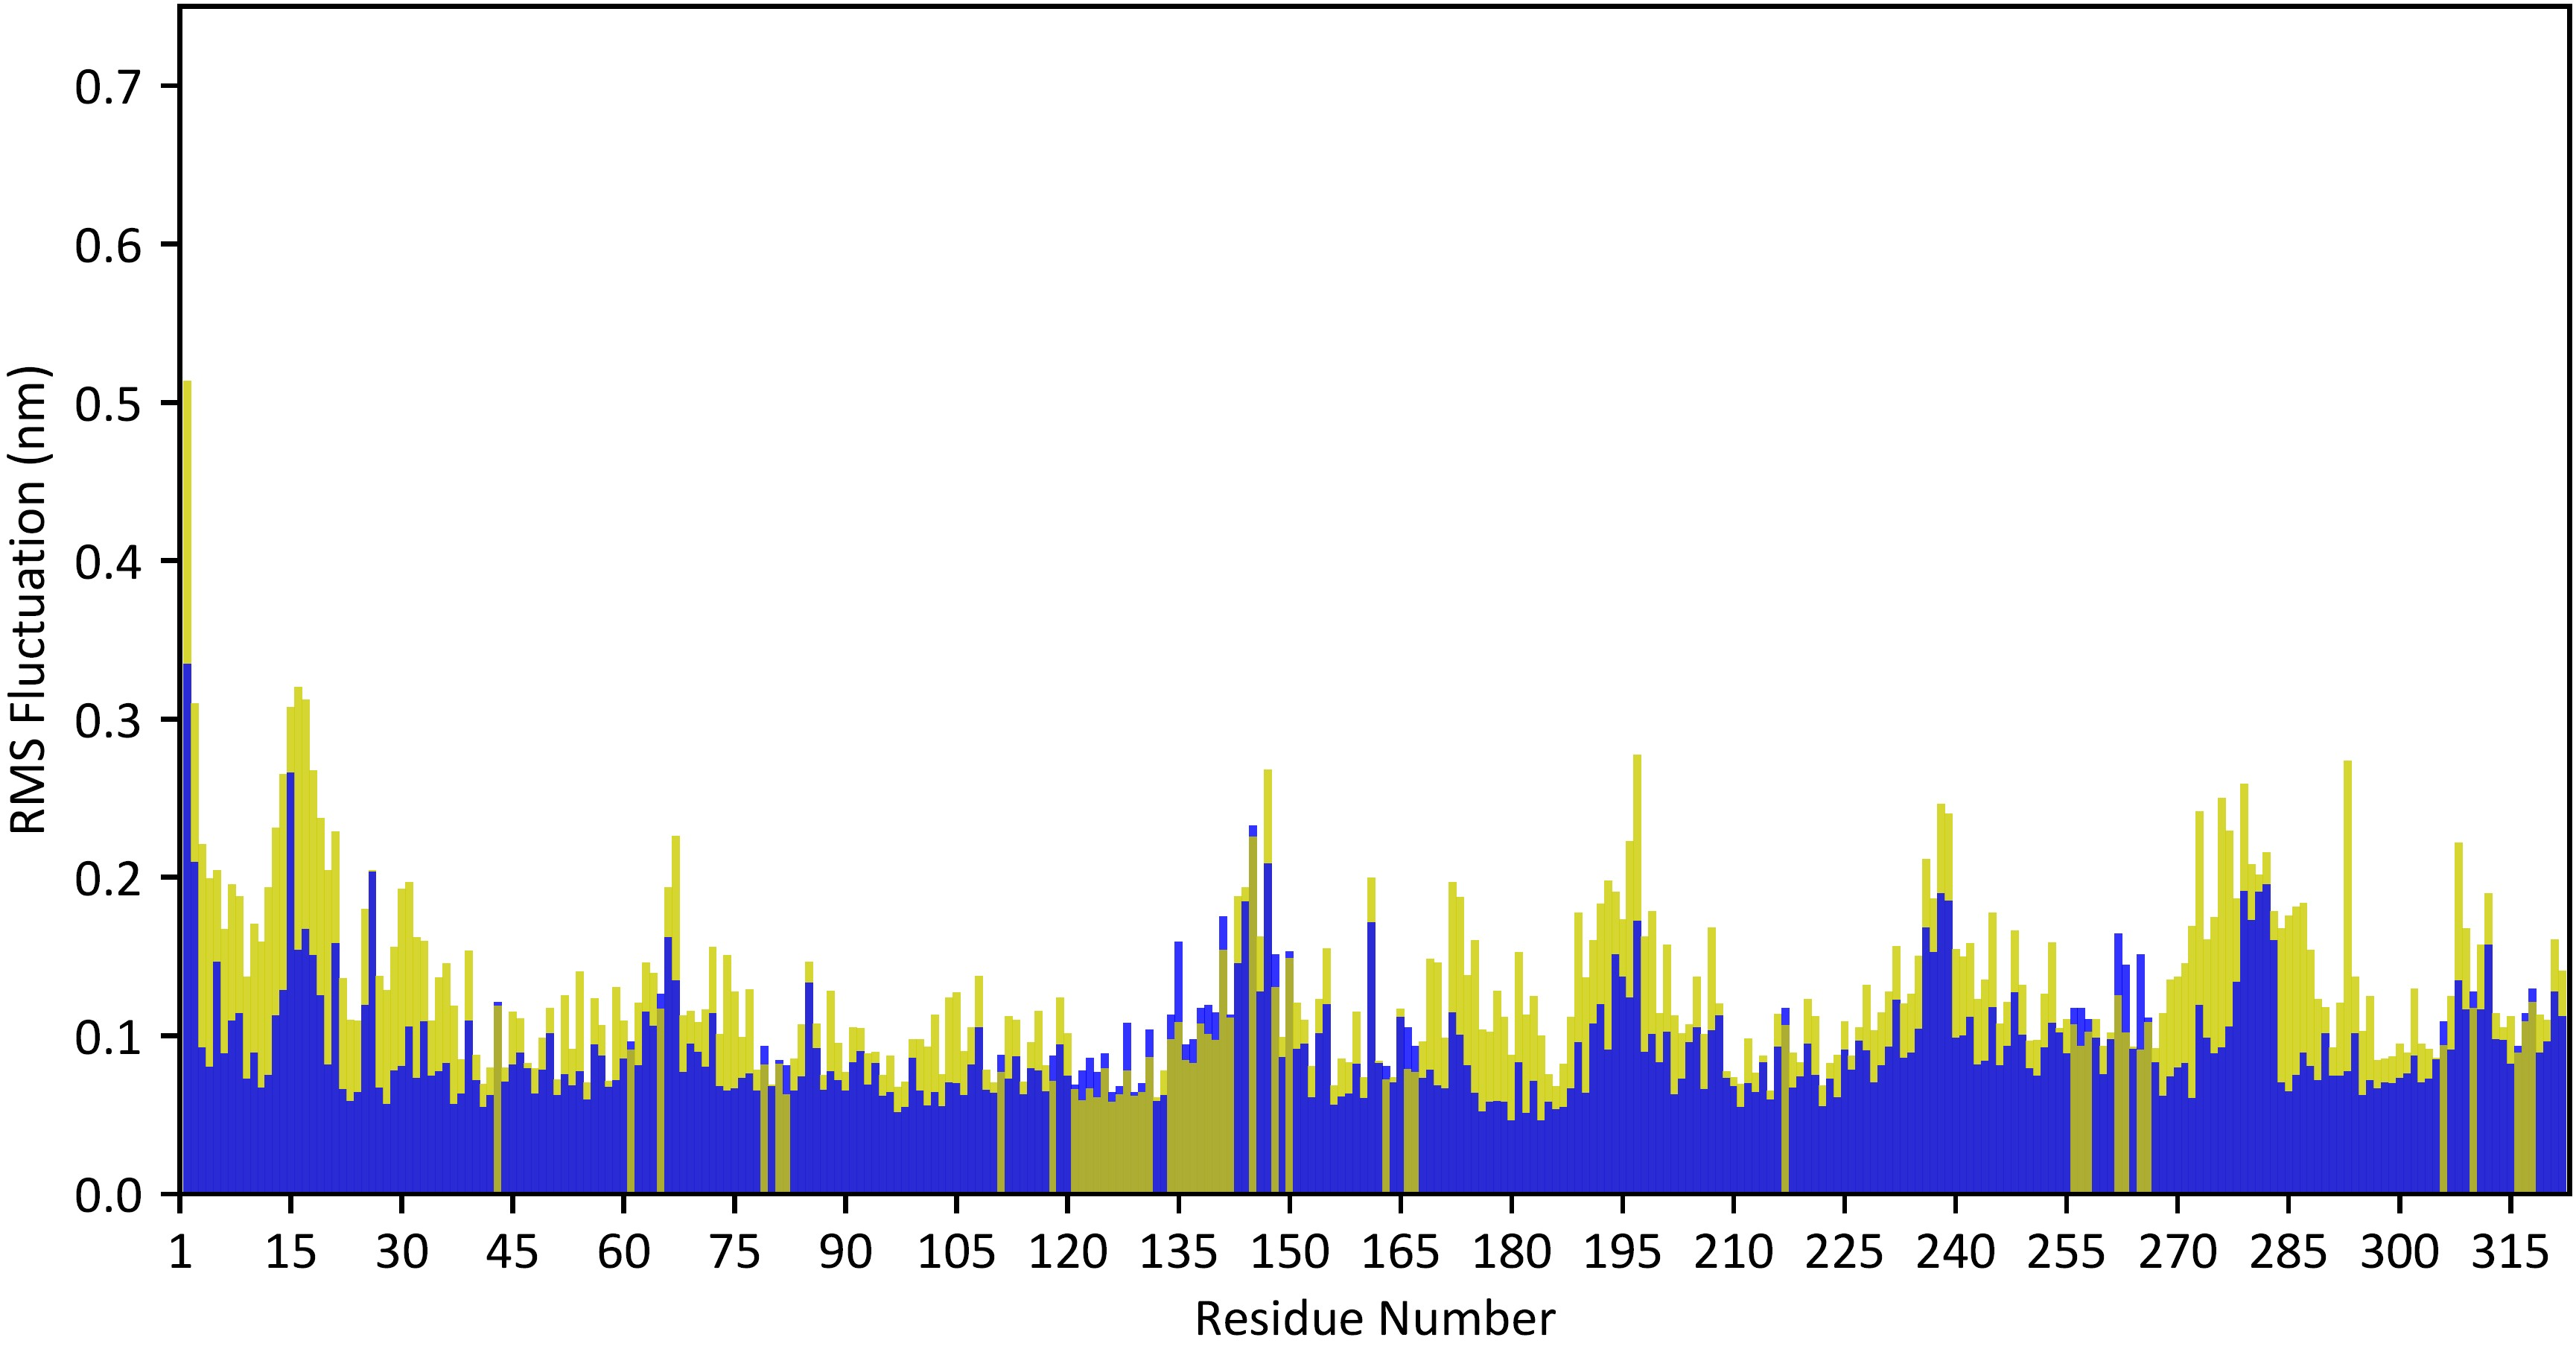
\includegraphics[width=\linewidth]{SuppFigures/wt rmsf.jpg}
    \textbf{b)} QTY-designed OPN2 \\ \\
    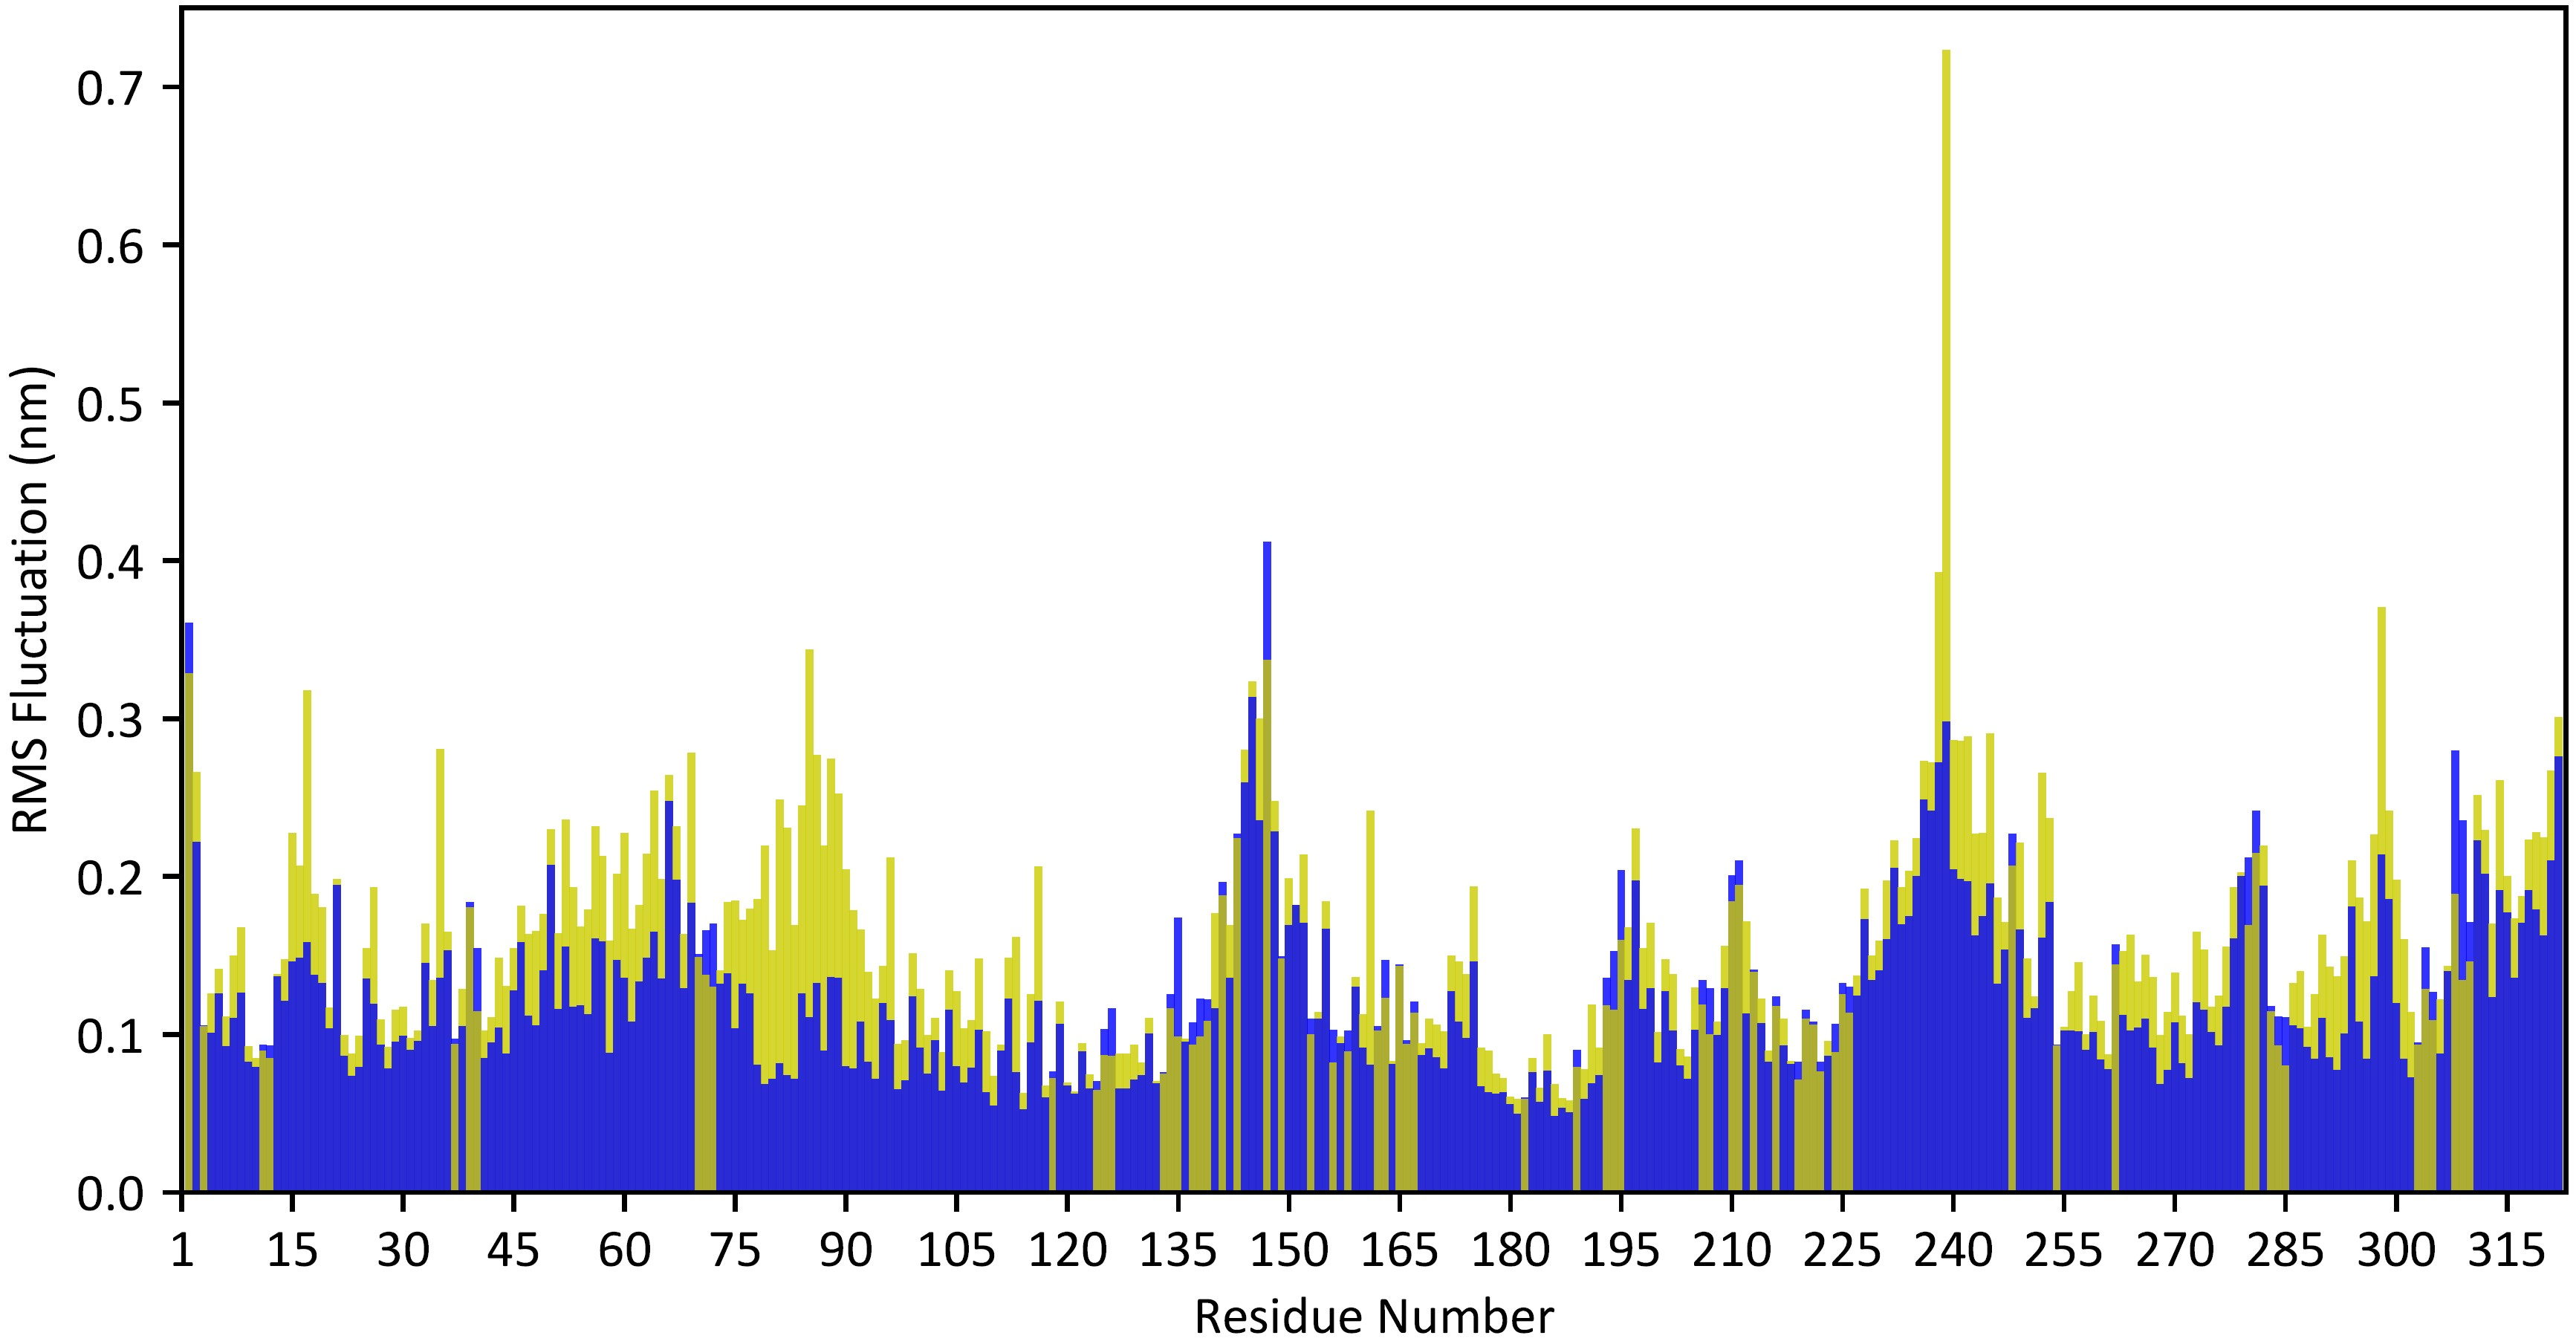
\includegraphics[width=\linewidth]{SuppFigures/qty rmsf.jpg}
\end{figure}

\begin{figure}[H]
    \caption{\textbf{The root mean square distance (RMSD) of each residue in the retinal-binding pocket of native and QTY-designed OPN2. } By convention, the isomerization is set at time 0ns, which is indicated by a brown, vertical dashed line. Only the 1-ns running average of RMSD are shown for clarity. }
    \textbf{a)} Native OPN2 \\ \\
    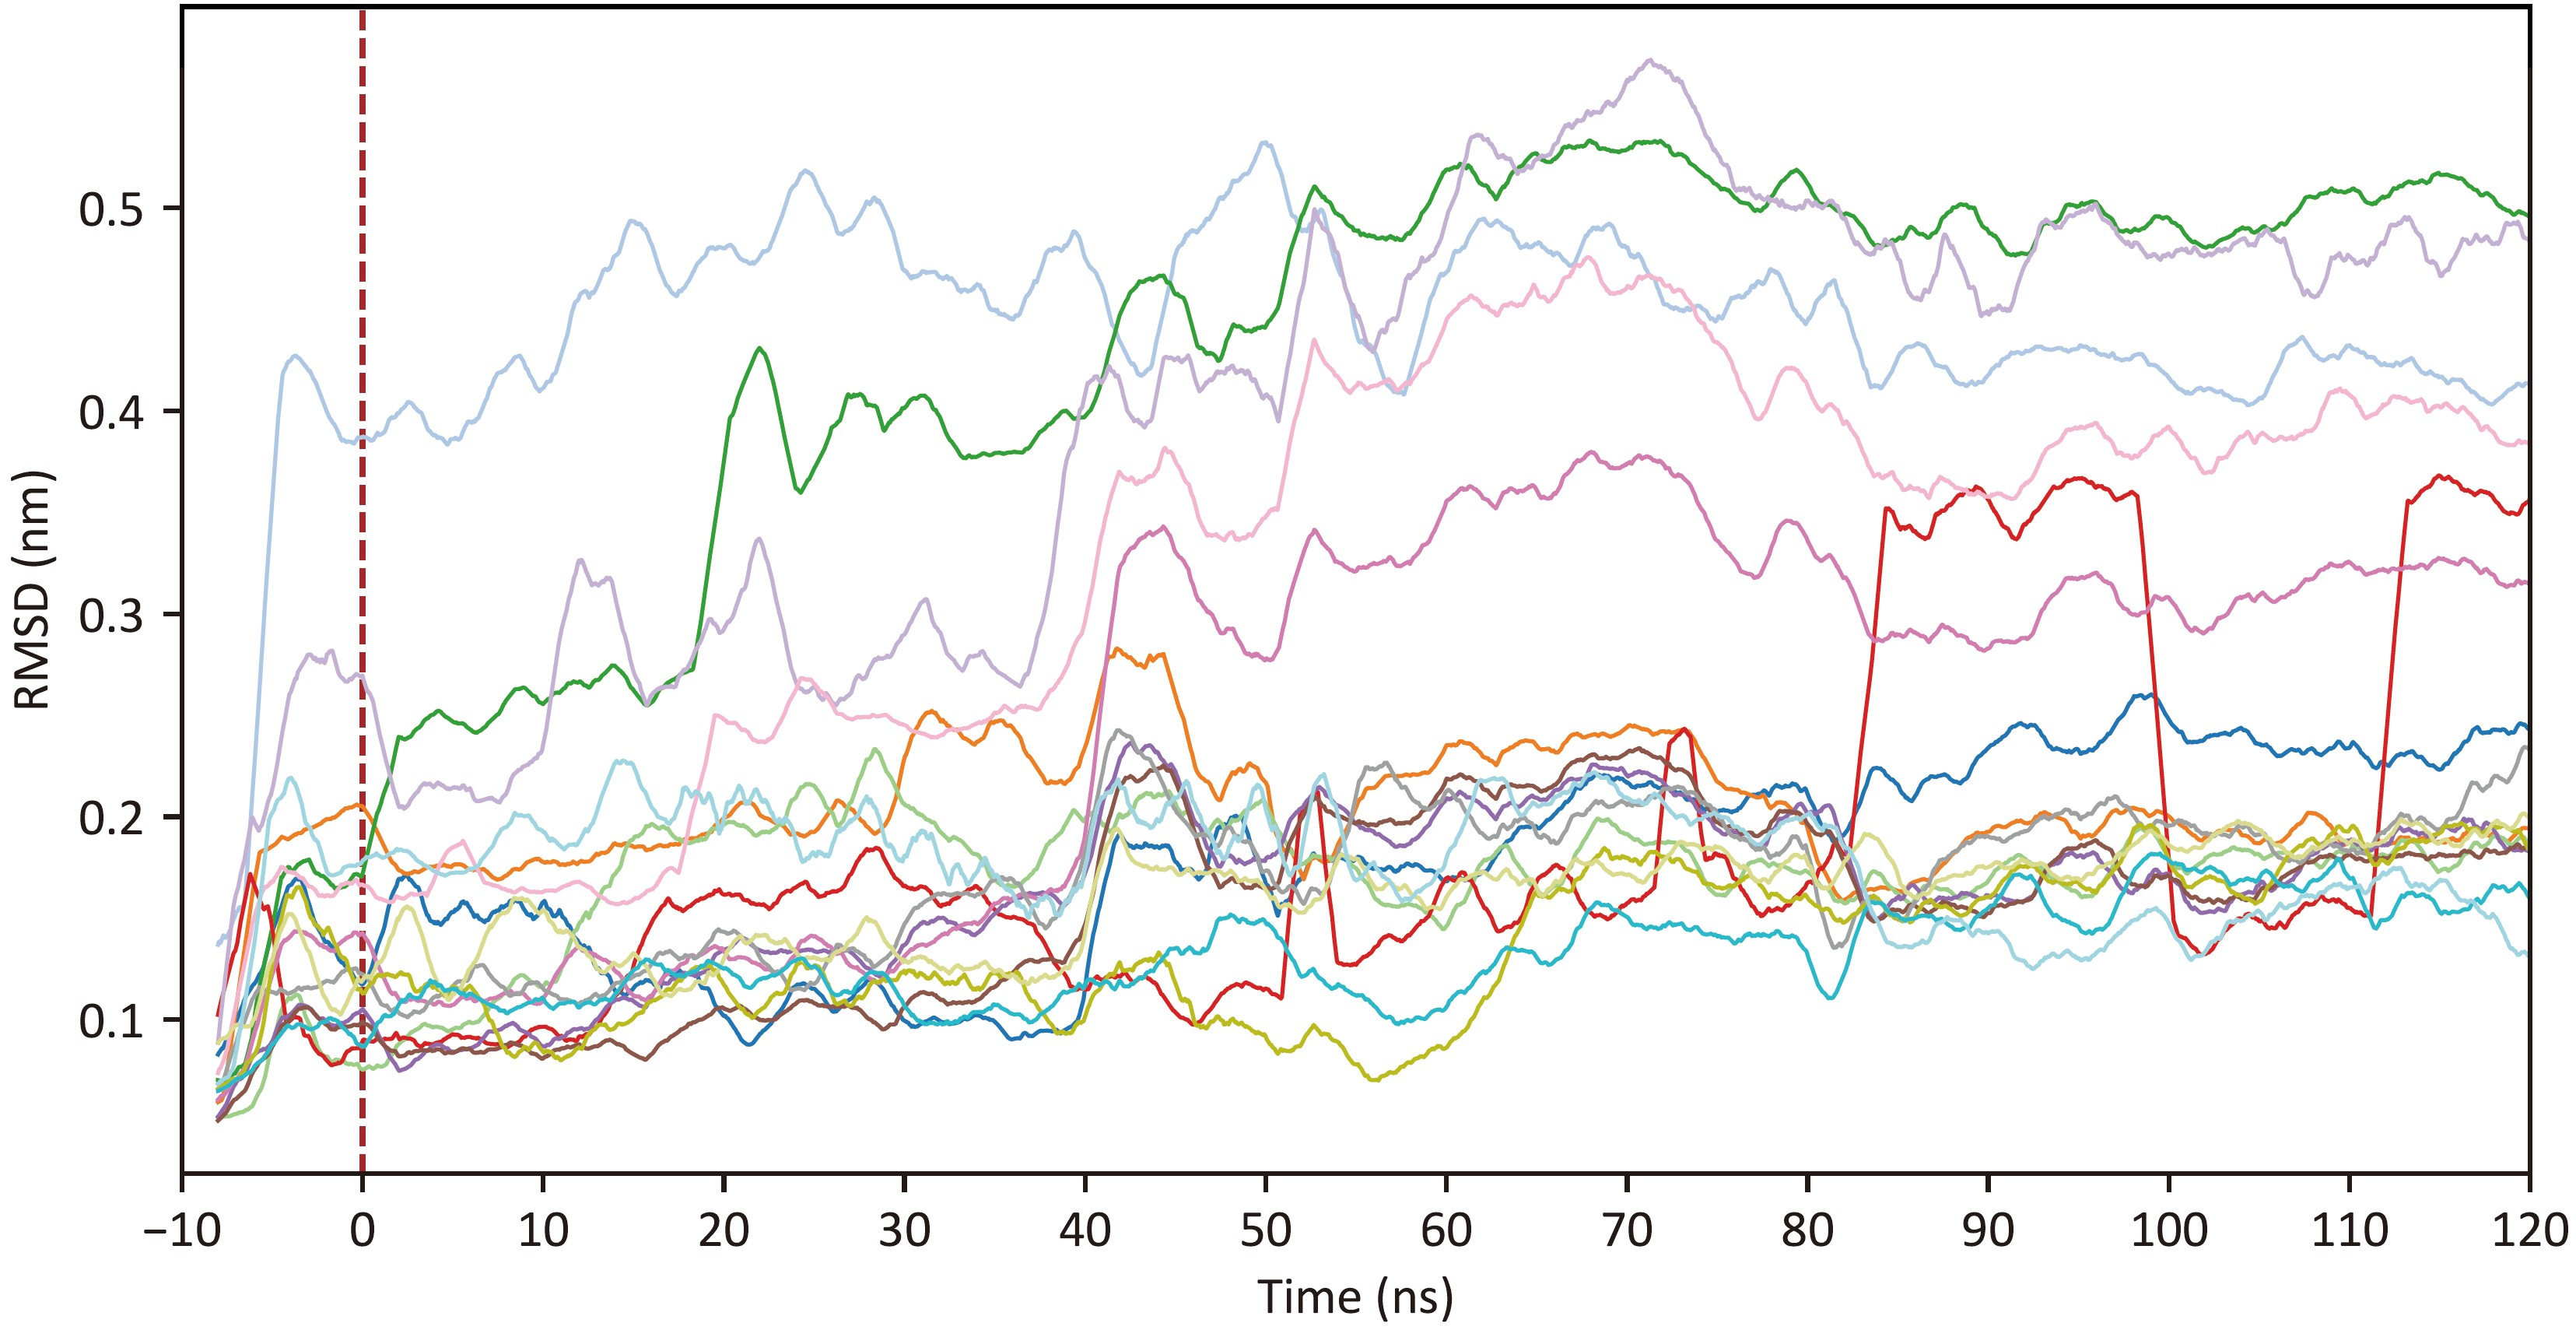
\includegraphics[width=\linewidth]{SuppFigures/wt rmsd byres.jpg}
    \textbf{b)} QTY-designed OPN2 \\ \\
    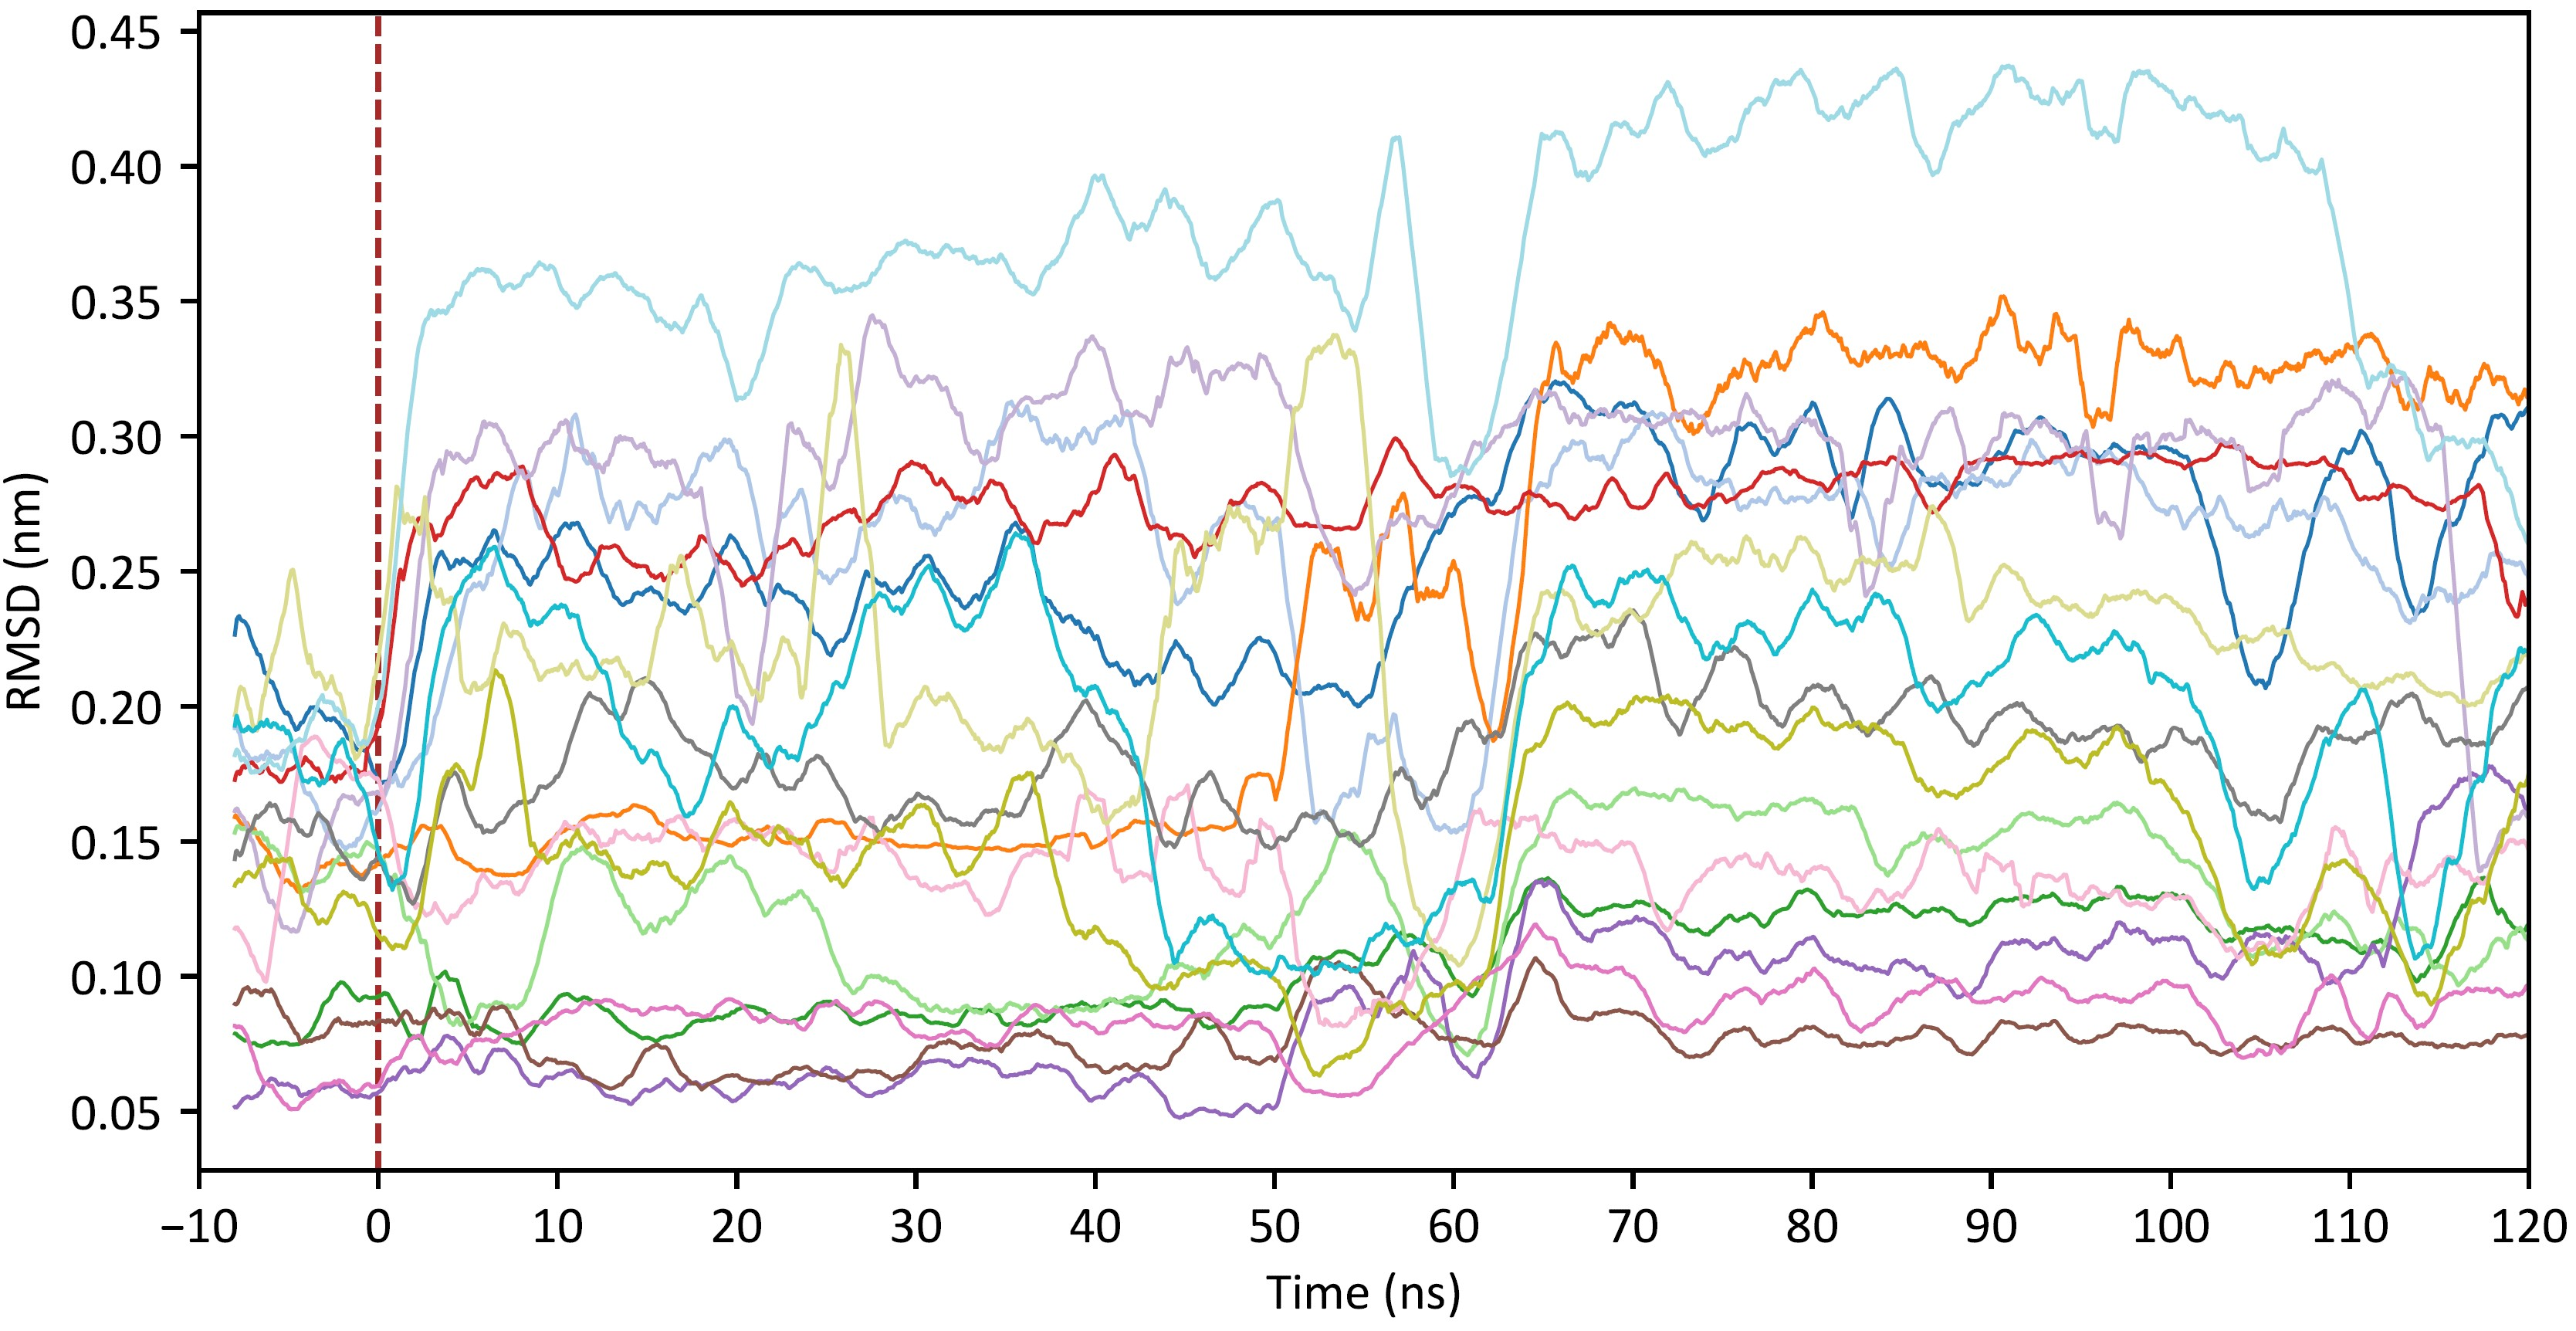
\includegraphics[width=\linewidth]{SuppFigures/qty rmsd byres.jpg}
    
    \vspace{0.5cm}
    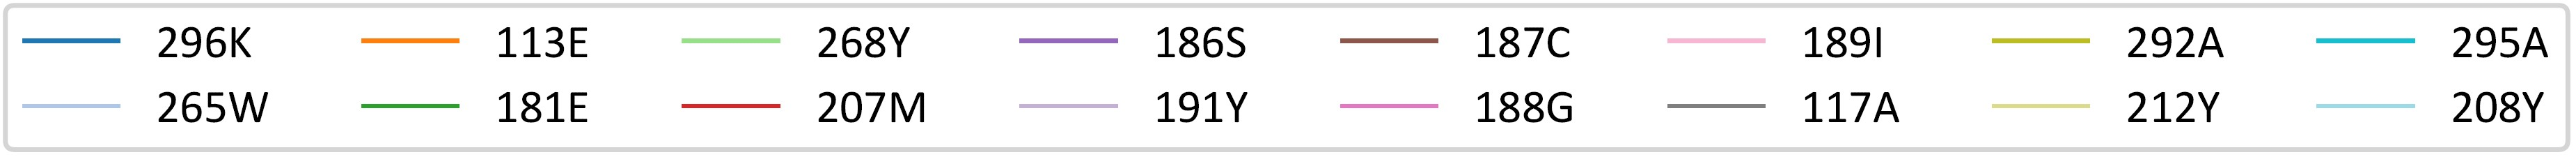
\includegraphics[width=\linewidth]{SuppFigures/legend rmsd byres.jpg}
\end{figure}

\end{document}